% Thesis root file. yay.

\documentclass[phys,dissertation,unsrt]{puthesis}

\usepackage{amsmath}
\usepackage{subfigure}
\usepackage{multicol}
\usepackage{multirow}
\usepackage{graphicx}
\usepackage{color}
\usepackage{natbib}
\usepackage{url}

\linespread{1.1}

\sloppy

% Put % at the end of the last line to avoid getting an extra space
% in the abstract.
\title{
	Novel Ideas and Techniques \\
	for Large Dark Matter Detectors%
}

\author{Darryl Masson}{Masson, Darryl}

\pudegree{Doctor of Philosophy}{PhD}{May}{2018}

\majorprof{Rafael F. Lang}

\campus{West Lafayette}

% defs
\newcommand{\n}[1]{\mathrm{#1}}    % normal (roman) text in math mode
\newcommand{\1}[1]{\, \mathrm{#1}}
\newcommand{\dd}{\mathrm{d}}
\newcommand{\order}{\mathcal{O}}
\newcommand{\degree}{{}^{\circ}}
\newcommand{\arxiv}[1]{\href{http://arxiv.org/abs/#1}{\texttt{arXiv:#1}}}
\newcommand{\keVnr}{$\mathrm{keV_{nr}}$}
\newcommand{\keVee}{$\mathrm{keV_{ee}}$}
\newcommand{\ua}{$\mathrm{U_{A^{\prime}}}(1)$}

\newcommand{\err}[2]{$#1\,\pm\,#2$}

\newcommand{\Rn}{${}^{222}$Rn}
\newcommand{\Po}{${}^{218}$Po}
\newcommand{\Pb}{${}^{214}$Pb}
\newcommand{\BiPo}{${}^{214}$BiPo}
\newcommand{\todo}[1]{\color{red}\textbf{#1}\color{black}}

\includeonly{chapter_dm}

\begin{document}

\volume

% Front matter (dedication, etc.).
% front matter

%\begin{document} 

 % Dedication page is optional.

  % Acknowledgements page is optional

  % The preface is optional.


  % The Table of Contents will be automatically created for you
  % using information you supply in
  %     \chapter
  %     \section
  %     \subsection
  %     \subsubsection
  % commands.
\tableofcontents

  % The List of Tables will be automatically created for you using
  % information you supply in
  %     \begin{table} ... \end{table}
  % environments.
\listoftables

  % The List of Figures will be automatically created for you using
  % information you supply in
  %     \begin{figure} ... \end{figure}
  % environments.
\listoffigures

  % List of Symbols is optional.
\begin{symbols}

$m$& mass\cr
$v$& velocity\cr

\end{symbols}

  % List of Abbreviations is optional.
\begin{abbreviations}

LXe& Liquid xenon\cr
GXe& Gasseous xenon\cr
TPC& Time projection chamber\cr
WIMP& Weakly interacting massive particle\cr
DM& Dark matter\cr
LNGS& Laboratori Nazionali del Gran Sasso

\end{abbreviations}

  % Nomenclature is optional.

  % Glossary is optional


  % Abstract is required.

\begin{abstract}

This is where the abstract goes.
Not much to say yet.

\end{abstract}

%\end{document}


% DM
% dark matter, v1.0

\chapter{The Case for Dark Matter}

\paragraph{Abstract} In this chapter we outline the evidence supporting the existence of dark matter, provide a brief discussion of possible models describing what dark matter might be, and review detection schemes.

\section{Evidence for Dark Matter}

For most of the last century evidence for the existence of dark matter has been gathering from various sources. In the 1920s Edwin Hubble showed conclusively that the universe was much more than just our Milky Way galaxy~\cite{Hubble:1929}. Very soon it became clear that the universe was a very large place and that we understood very little about it.

\subsection{Galactic Rotation curves}

In the early 17th century Johannes Kepler published his three laws of planetary motion~\cite{Kepler}. Kepler's Third law is easily derived with the help of Newtonian gravitation and centripetal motion for the case of a circular orbit:
\begin{equation} \label{eq:rotation_curve}
\frac{a^3}{T^2} = \frac{GM}{4\pi^2} \Longrightarrow v(r) = \sqrt{\frac{GM}{r}}
\end{equation}
where $a$ is the orbital semimajor axis ($r$ if circular), $T$ the orbital period, $G$ the gravitational constant, $M$ the mass of the central body, and $v$ the orbital speed (assuming a circular orbit). If we assume the mass distribution is a function purely of radius, we can define
\begin{equation} \label{eq:mass_distribution}
M(r) = \int_0^r \dd^3r^{\prime}\, \rho (r^{\prime}) = 4\pi\,\int_0^r \dd r^{\prime}\, r^{\prime 2} \rho(r^{\prime})
\end{equation}
and generalize the expression Kepler found to give us a relationship relating the expected orbital velocity of an object in a galaxy as a function of its distance from the galactic core.

Armed with equations~\eqref{eq:mass_distribution} and~\eqref{eq:rotation_curve}, we can calculate $M(r)$ by observing a galaxy with telescopes and assuming some stellar mass distribution, and then make some prediction for $v(r)$. Using Doppler-shifted lines of stars or dwarf galaxies, the orbital velocities can be measured and compared to the prediction from the mass distribution, as seen in figure~\ref{fig:rotation_curve} from the Triangulum galaxy (M33)~\cite{Corbelli:1999af}.

\begin{figure}[htb]
\centering
    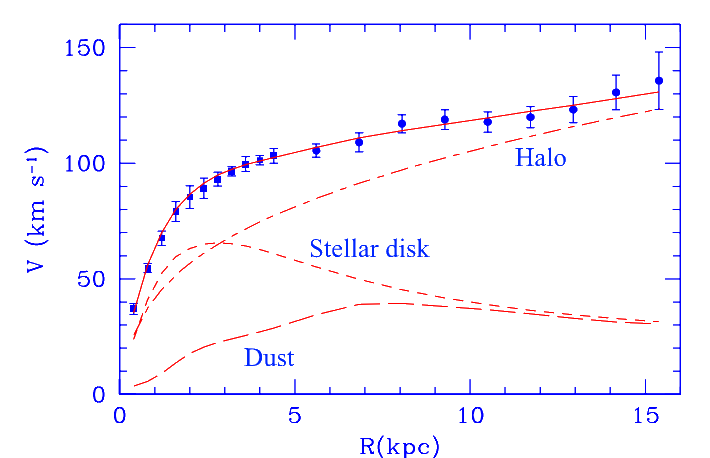
\includegraphics[width=0.8\textwidth]{figures/dm/m33_rotation}
    \caption{Rotation curve of M33, from~\cite{Corbelli:1999af}. The measured rotation speeds cannot be explained by the observed distribution of stars and dust and require the addition of a hidden source of mass to reproduce the observations.}\label{fig:rotation_curve}
\end{figure}

If we assume that stars, gas, dust, and other objects visible with telescopes are the dominant components of the galaxy, then at large distances from the galactic center it will increasingly appear like a point mass, giving the familiar relationship $v(r) \sim r^{-1/2}$ that is Kepler's third law. In the bulge at the center of the galaxy, we see the speed increases roughly linearly with the radius, while at large radii the velocity is approximately constant or increasingly slowly. However, the mass required to produce this effect is not evident in any telescope. Additionally, the stars near the edge of the galaxy are well above the predicted escape velocity $v_{\n{esc}} = \sqrt{2}v_{\n{circ}}$. Galaxies are stable over astronomical periods of time, so they cannot be filled with objects exceding the escape velocity. From this, we can propose some mass distribution that has a negligible contribution in the inner parts of the galaxy but becomes dominant at large radii~\cite{Navarro:1995iw,Graham:2005xx}.

\subsection{Gravitational lensing}

One prediction of Einstein's Theory of General Relativity is that any concentration of matter and energy will act as a lens for passing photons by distorting spacetime~\cite{Einstein:1936}. The amount and manner of lensing observed indicates the amount of matter present.

\subsubsection{Strong lensing}

Strong lensing is when images of background galaxies experience significant distortion or form multiple images by foreground objects. A good example is Einstein's Cross (QSO 2237+0305)~\cite{einstein_cross}, as shown in Figure~\ref{fig:einstein_cross}, where a distant quasar forms four images around a foreground galaxy.

\begin{figure}[htb]
    \centering
    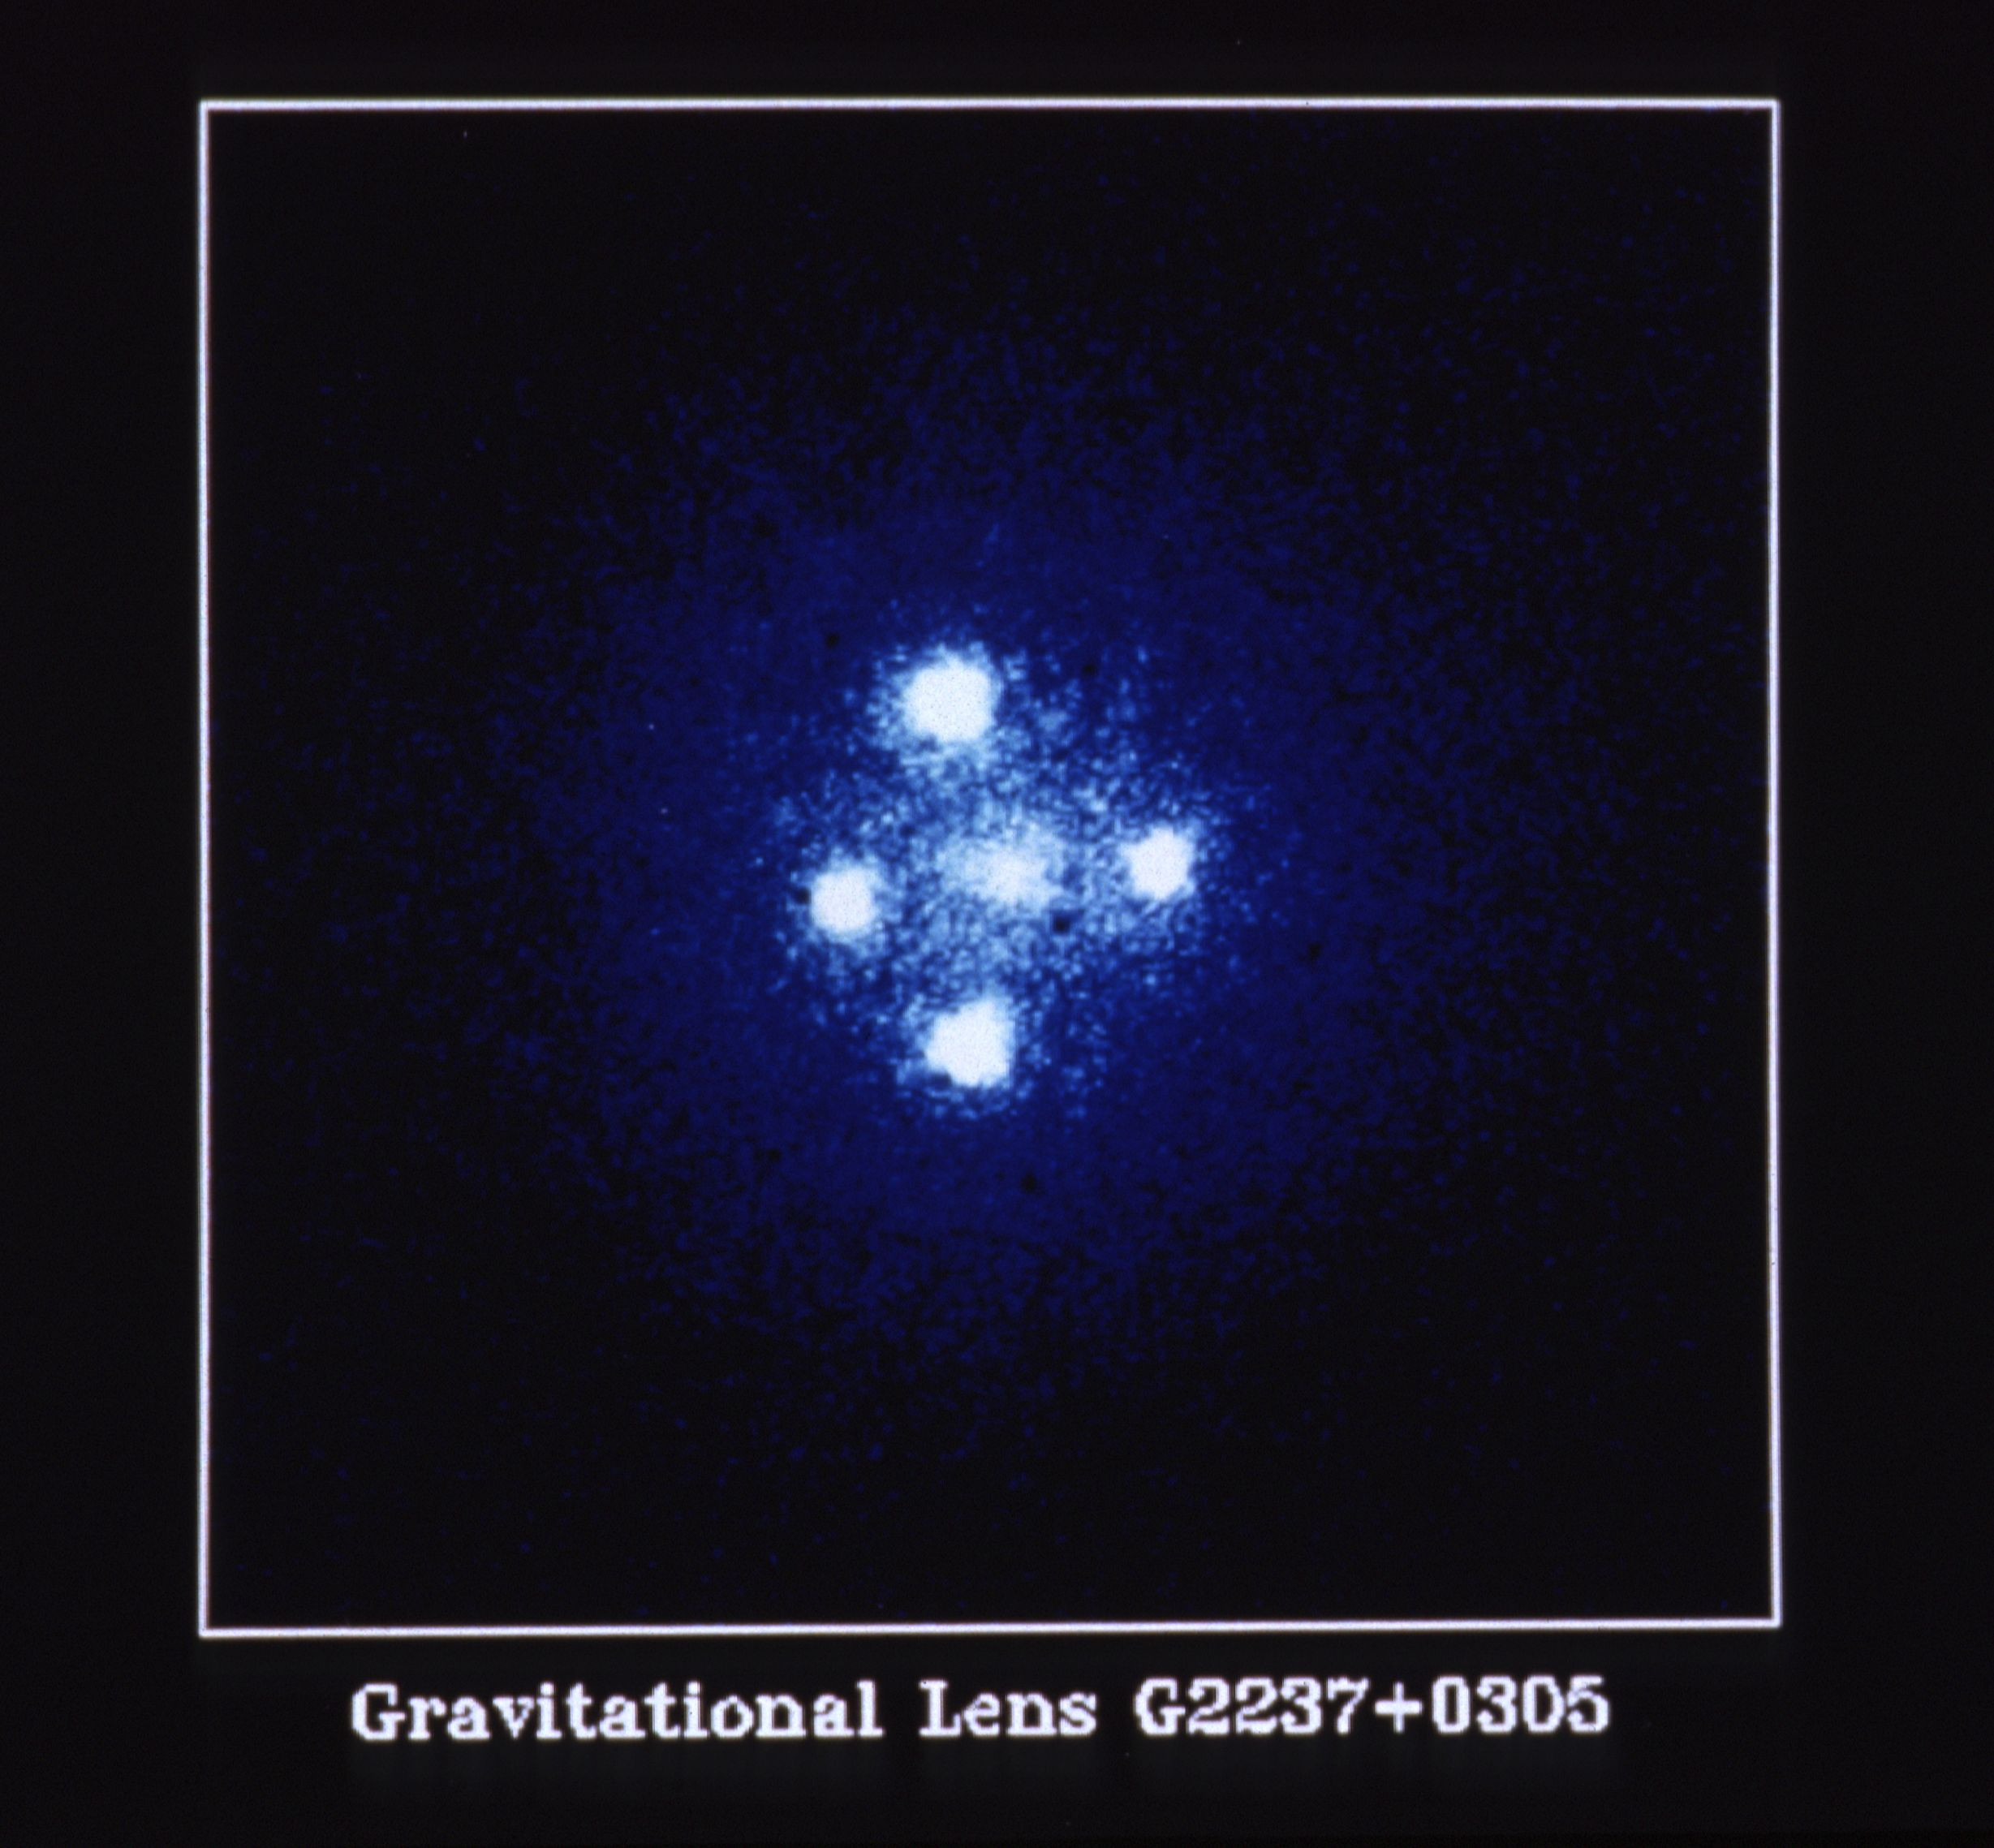
\includegraphics[width=0.8\textwidth]{figures/dm/einstein_cross}
    \caption{The Einstein's Cross, QSO 2237+0305. A distant quasar forms multiple images when lensed around a foreground galaxy. Image from HST~\cite{einstein_cross}.}\label{fig:einstein_cross}
\end{figure}

\subsubsection{Weak lensing}

In cases where the lensing object is not sufficiently dense or massive to create obvious strong lensing, weak lensing can still be observed. Weak lensing can be measured using statistical methods by creating an average shape of a galaxy in the field of view and calculating some distortion parameter~\cite{Bartelmann:1999yn}. A distribution of distortion can be created, which will indicate the locations of the greatest concentrations of mass. The analysis shows that the amount of mass observable is insufficient to account for the amount of lensing observed.

\subsection{Galaxy cluster dynamics}

\subsubsection{Virial theorem}

Observating the dynamics of galaxy clusters also yields fairly clear indication that dark matter must form a significant contribution to the mass of a galaxy cluster. When observations are made of clusters other than our own Local Group, a very large mass of diffuse hydrogen is observed in the space between galaxies. This hot gas radiates x-rays (and thus is often called hot x-ray gas), and from its luminosity both the temperature and mass can be measured. The extremely high temperatures observed result from basic energy conservation. As the gas falls into the cluster's gravitational potential well, it gains kinetic energy, which is equivalent to temperature. The temperature of the gas, indicated by its radiation spectrum, thus gives an indication of the depth of the potential well. Additionally, by applying the Virial theorem (2K~+~U~=~0)~\cite{Claussius:1870} to the cluster, the kinetic energies of the component galaxies can be measured and compared to the potential energy due to the visible mass. In both cases, the required potential well is much deeper than could be formed from merely the hot gas and the galaxies themselves, despite the fact that there is an order of magnitude more mass in gas than in galaxies. Indeed, the extra mass required to make the system behave is an order of magnitude greater than the observable mass in galaxies and gas.

\subsubsection{Bullet cluster}

The Bullet Cluster (1E 0657-558) is an excellent example of both galaxy cluster dynamics and weak lensing, and also furnishes additional information on dark matter. Figure~\ref{fig:bullet_cluster} is a composite image from Hubble Space Telescope (HST), Chandra X-ray Observatory, and Magellan. The pink is the hot x-ray gas (seen by Chandra), and forms the majority of the baryonic mass of the cluster. The powerful shock produced during the collision is clearly seen in the subcluster on the right, giving indications of the speed of the collision, and also the mass of that subcluster. The blue regions, centered on the visible galaxies, show the computed weak lensing centers.

\begin{figure}[htb]
\centering
   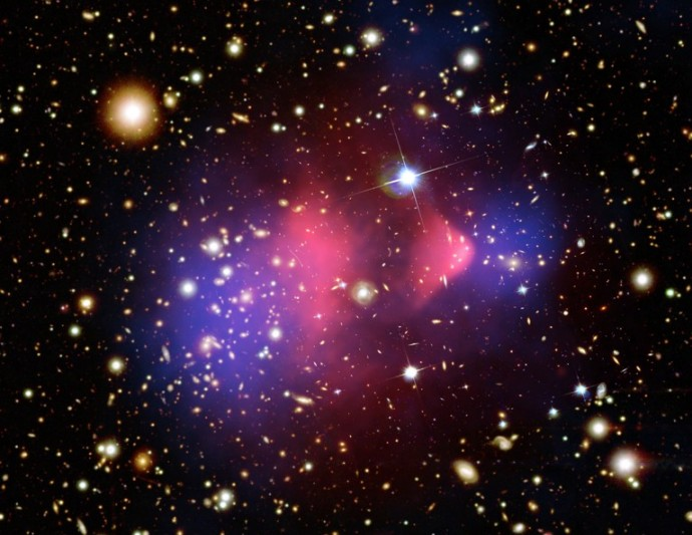
\includegraphics[width=0.8\textwidth]{figures/dm/bullet_cluster}
   \caption{The Bullet Cluster of galaxies, from~\cite{bullet}. Two subclusters passed through each other without significantly affecting the constituent galaxies, however the hot x-ray gas (pink) experienced significant disruption and was pulled away. Despite the majority of visible mass being contained within the gas, a lensing study reveals that the lensing centers (blue) are still centered on the galaxies, indicating that the intracluster gas, while dominating the baryonic mass, is not a major component of the total cluster mass, and also that this invisible matter does not experience significant self-interactions~\cite{Kahlhoefer:2013dca}.}\label{fig:bullet_cluster}
\end{figure}

When the two subclusters passed through each other, the constituent galaxies passed each other with minimal interaction. The two volumes of intracluster gas, being large balls of plasma, experienced significant drag, and the gas separated from the galaxies. A weak lensing study reveals that the lensing centers are still located around the galaxies, even though the mass of the intracluster gas greatly exceeds that of the stars and dust. From this we conclude that the majority of the mass of the subclusters is contained in this invisible matter, and also that it does not experience significant self-interactions~\cite{Kahlhoefer:2013dca}.

\subsection{Structure formation}

After the creation of atoms some $400\,000$ years following the Big Bang, larger structures started forming under the influence of gravity. Any region of slightly higher density started accumulating more matter. This process can be simulated by starting from measurements of the density of the early universe (discussed below) and propagating interactions of gravity and electromagnetism over time. While the computational cost of simulating the universe is, predictably, quite high, this has been done with great success by the Millenium~\cite{Springel:2005nw}, Illustris~\cite{Genel:2014lma,Vogelsberger:2014dza,Sijacki:2014yfa}, and IllustrisTNG~\cite{Pillepich:2017jle} projects. The results found by these simulations is that the large scale structure observed in the universe does not form under the interaction of baryonic matter alone. The inclusion of dark matter is necessary for these structures to form. Indeed, the structures observed in these simulations, as shown in Figure~\ref{fig:structure}, bears very strong resemblance to what is seen with telescopes.

\begin{figure}[htb]
    \centering
    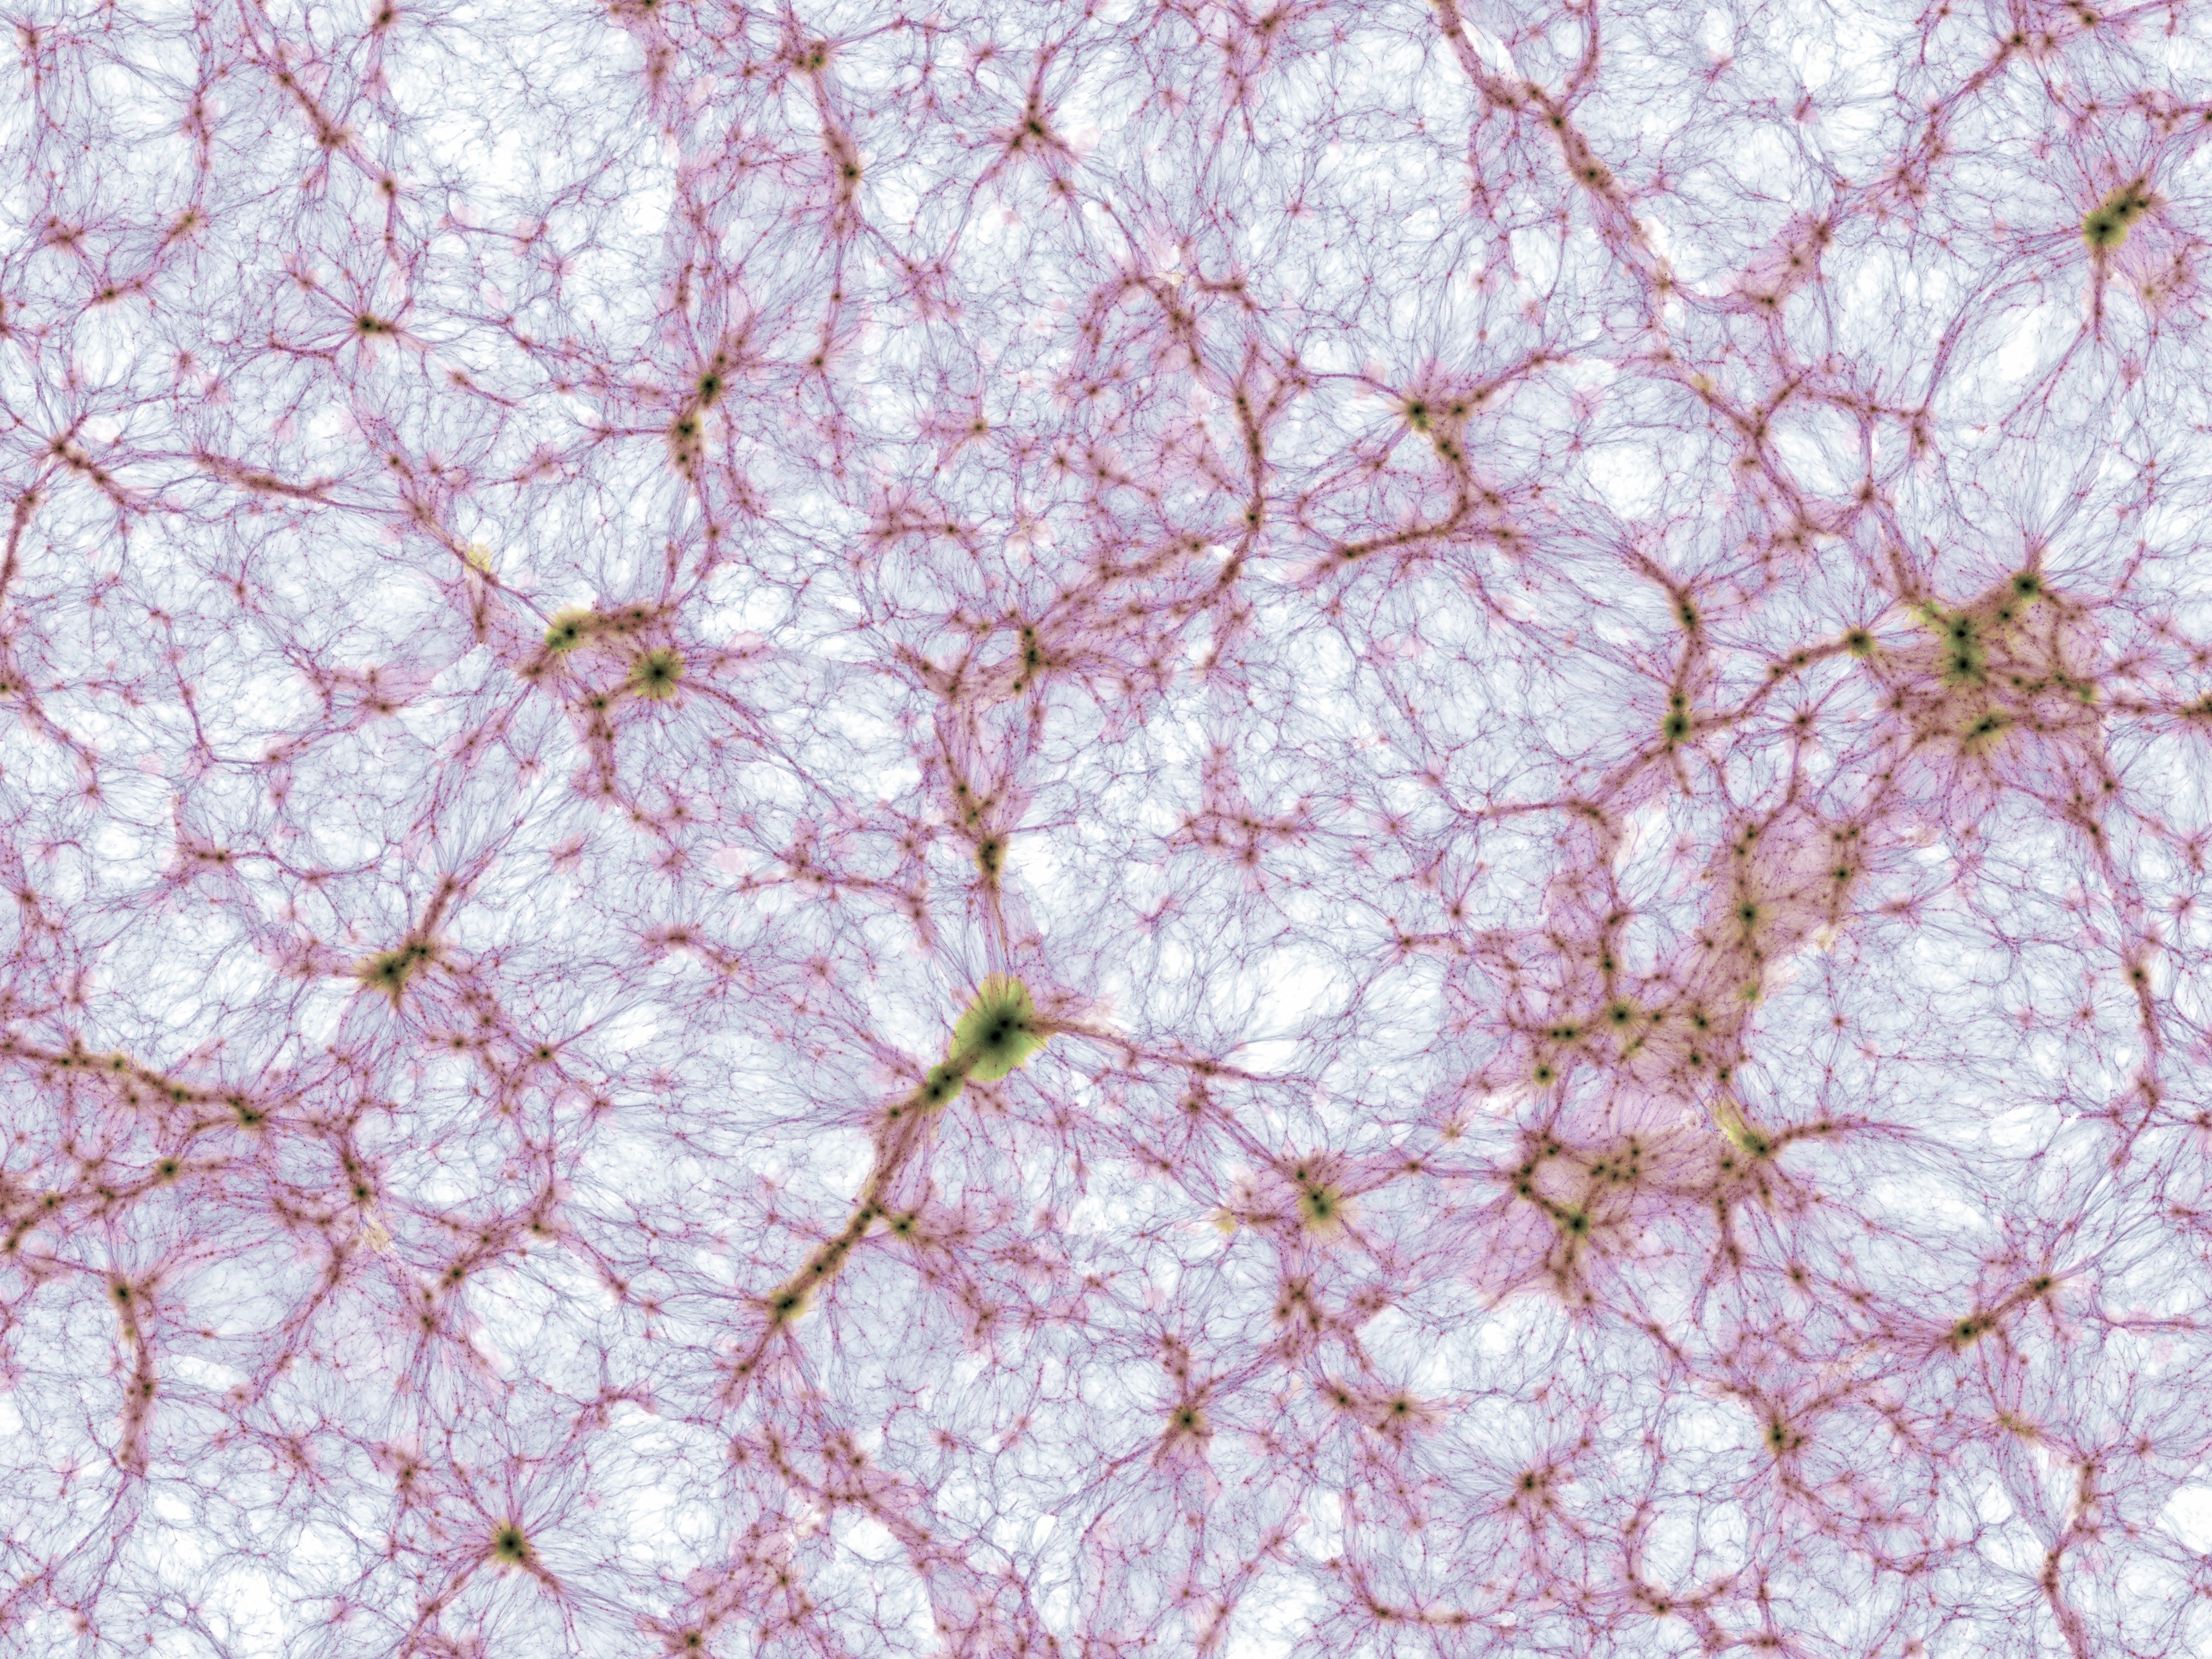
\includegraphics[width=0.8\textwidth]{figures/dm/TNG300_gas_dens_temp_hr}
    \caption{An image from the TNG300 simulation of IllustrisTNG~\cite{Pillepich:2017jle} showing the baryon density and the gas temperature. Without the inclusion of a significant quantity of dark matter, the kind of structure observed in the universe does not form.}\label{fig:structure}
\end{figure}

\subsection{Cosmic Microwave Background (CMB)}

Penzias and Wilson were the first to turn a sensitive microwave telescope to the skies~\cite{Penzias:1965a,Penzias:1965b}, and their discovery earned them the Nobel Prize in Physics in 1978. The best measurements of the CMB come from satellites like Wilkinson Microwave Anisotropy Probe (WMAP)~\cite{Bennett:2012zja} and Planck~\cite{Ade:2015xua}, and are (at face value) featureless and isotropic to a few parts per million as shown in Fig.~\ref{fig:cmb}a. After the subtraction of the average, dipole, and galactic contributions, we get Fig.~\ref{fig:cmb}b.

\begin{figure}[htb]
    \begin{tabular}{cc}
    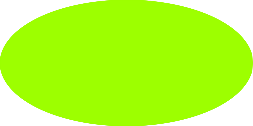
\includegraphics[width=0.5\textwidth]{figures/dm/CMB0} & 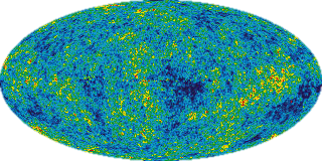
\includegraphics[width=0.5\textwidth]{figures/dm/CMB3} \\
    \end{tabular}
    \caption{(Left) The cosmic microwave background radiation as measured by WMAP~\cite{Bennett:2012zja}. The temperature of the universe is flat and lacking any features above the a few parts per million. (Right) After subtracting the contributions from various backgrounds, we see the temperature profile of the universe at the moment when photons decoupled from baryons about $380\,000$ years after the Big Bang. Hotter regions had a greater concentration of the primordial soup and formed from quantum fluctuations in the early universe.}\label{fig:cmb}
\end{figure}

Certain regions radiate at a slightly higher temperature, indicating a greater concentration of the soup of baryons and photons in the early universe. These differences arose due to quantum fluctuations during the early expansion. This temperature map can be expanded in the spherical harmonics and a power spectrum plotted, as shown in Figure~\ref{fig:cmb_ps}. Various cosmological models can be tested by fitting to this spectrum.

\begin{figure}[htb]
\centering
    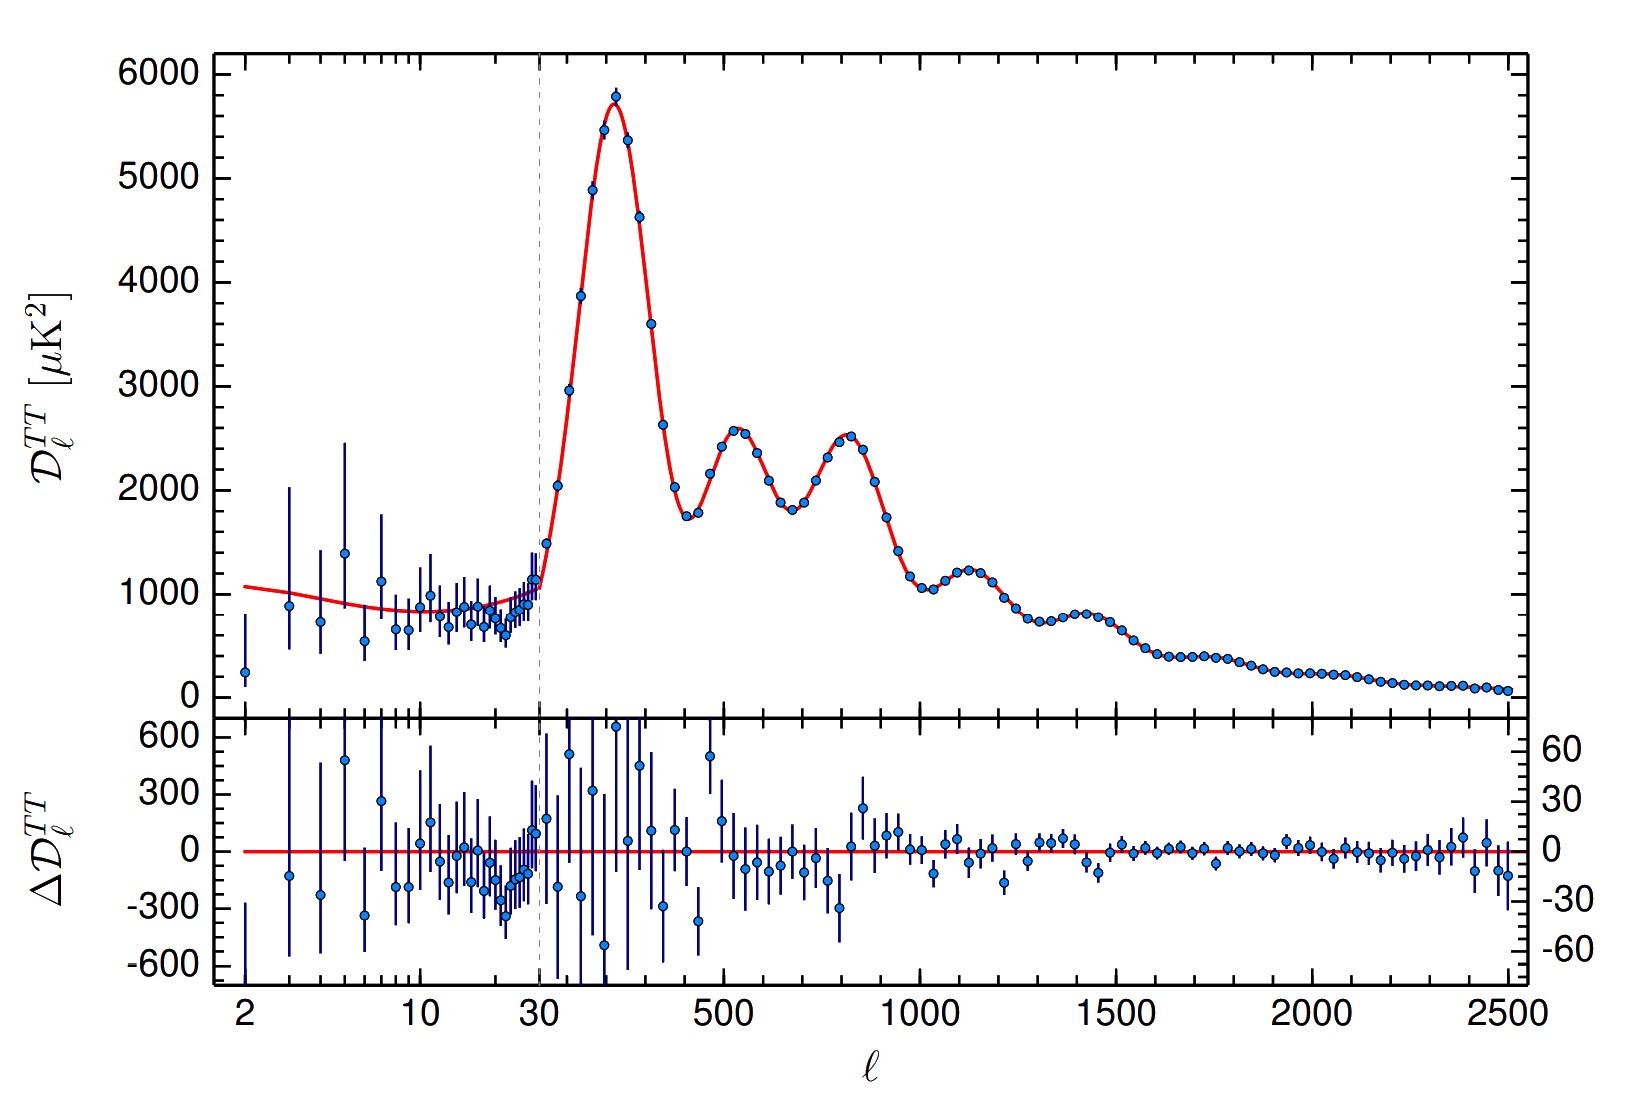
\includegraphics[width=0.8\textwidth]{figures/dm/planck2015_cmb}
    \caption{The power spectrum of the spherical harmonic expansion of the CMB from Planck~\cite{Ade:2015xua}. The lack of damping on the third peak indicates significant contributions to the universe from non-baryonic matter.}\label{fig:cmb_ps}
\end{figure}

The model with the best fit is $\Lambda$CDM, which at its simplest is a six-parameter model that describes the universe as filled with cold (non-relativistic) dark matter (CDM) with additional contributions from dark energy ($\Lambda$)~\cite{Riess:1998cb}. From the results extracted from the fit we learn a variety of things about the universe. Of key importance are contributions to the total energy content of the universe. According to Planck~\cite{Ade:2015xua}, the baryonic fraction $\Omega_b$ is merely $0.049$, the dark matter fraction $\Omega_{\n{DM}}$ $0.265$, and the dark energy fraction $\Omega_{\Lambda}$ $0.686$. Thus, the majority of the universe is not of a baryonic nature.

\subsection{Big Bang Nucleosynthesis (BBN)}

Within a minute after the Big Bang, the universe had cooled sufficiently to allow nuclei to form and not be immediately broken apart due to the high ambient temperature. Neutrons and protons had just fallen out of numerical equilibrium due to their small difference in mass, and now existed in a ratio of about 1 neutron per 7 protons. Neutrons and protons first combined to make deuterium, then as the deuterium abundance increased, deuterium fused with deuterium to produce tritium and helium-3 and then with tritium to produce helium-4. This epoch continued for just under half an hour, until expansion had driven particles far enough apart that collisions became infrequent and cooling robbed the collisions of sufficient energy to initiate the reactions. At this point, the majority of the universe's neutrons were in helium due to its stability, and of the few remaining, most were in deuterium. Due to the weak binding of deuterium, a universe with more photons will contain more photons with sufficient energy to disassociate the deuterium, so mean fewer deuterium nuclei survive this epoch. Due to its stability, the population of $^4$He depends very little on the photon density. By measuring the primordial abundance of deuterium, this will admit a value of the ratio between nuclei and photons, which will in turn indicate what percentage of the universe was baryonic in this epoch.

By comparing the prediction from theory with measurements (Ref~\cite{Steigman:2007xt}, see also Figure~\ref{fig:bbn}), we can place a stringent requirement on the baryonic density of the universe to $\eta = (6.11\pm2.0)\times10^{-10}$, where $\eta$ is the ratio between the number of baryons and photons. This value of $\eta$ indicates that the majority of the universe is not of a baryonic nature.

\begin{figure}[htbp]
\centering
    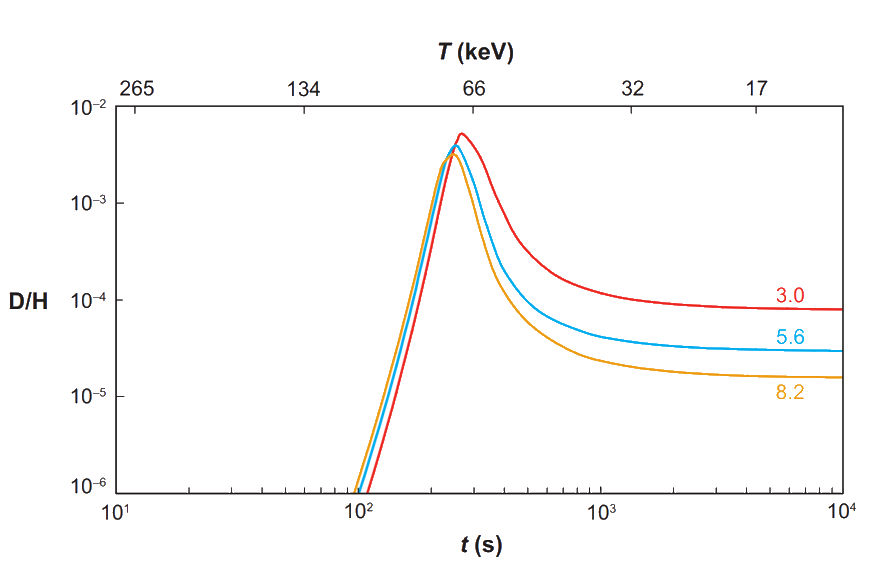
\includegraphics[width=\textwidth]{figures/dm/bbn_eta}
    \caption{The evolution of the relative abundance of deuterium depends strongly on the ratio between baryons and photons in the early universe. Deuterium forms from hydrogen, then combines with deuterium to form helium-3 and tritium or with tritium to form helium-4. Due its weak binding, deuterium is an excellent probe of the photon density. Measuring the deuterium abundance in the early universe admits a value of the baryon density during this epoch, which indicates that only a small fraction of the universe is baryonic. Figure from~\cite{Steigman:2007xt}.}\label{fig:bbn}
\end{figure}

\section{Searching for Dark Matter}

To search for dark matter, we need some ideas of what to look for. While we don't know what dark matter is, we can still start from things we already know about astrophysics and particle physics. We know any dark matter must be gravitationally bound to the Milky Way, which limits the maximum velocity to be escape velocity from the galaxy $v_{esc} \approx 600\1{km/s}$. Moreover, we know that dark matter does not experience significant self-interactions, and must have a long lifetime compared to the age of the universe. Additionally, we know that there must be some physics beyond the Standard Model.

The traditional approach has been to assume strong priors from both cosmology and particle physics, where a thermal relic particle and weak-scale physics beyond the standard model (BSM) like supersymmetry combine to give to the Weakly Interacting Massive Particle (WIMP)~\cite{Jungman:1995df}, on which we will primarily focus.

If we relax the strong particle physics prior, we have a generic thermal or quasi-thermal relic particle.

Relaxing just the cosmological physics prior proposes the QCD axion, first proposed to solve the strong CP problem~\cite{Peccei:1977,Weinberg:1978,Wilczek:1978}, as a dark matter candidate. Despite having very low masses ($10^{-12}\1{eV}$ to $10^{-2}\1{eV}$), the production mechanism of axions~\cite{Preskill:1983,Abbott:1983,Dine:1983} allows them to be created cold.

By assuming some unknown interaction mechanism between dark matter particles and standard model particles, we can draw a Feynman diagram to represent possible ways to investigate the nature of dark matter, as shown in Figure~\ref{fig:feynman}.

\begin{figure}[htb]
    \centering
    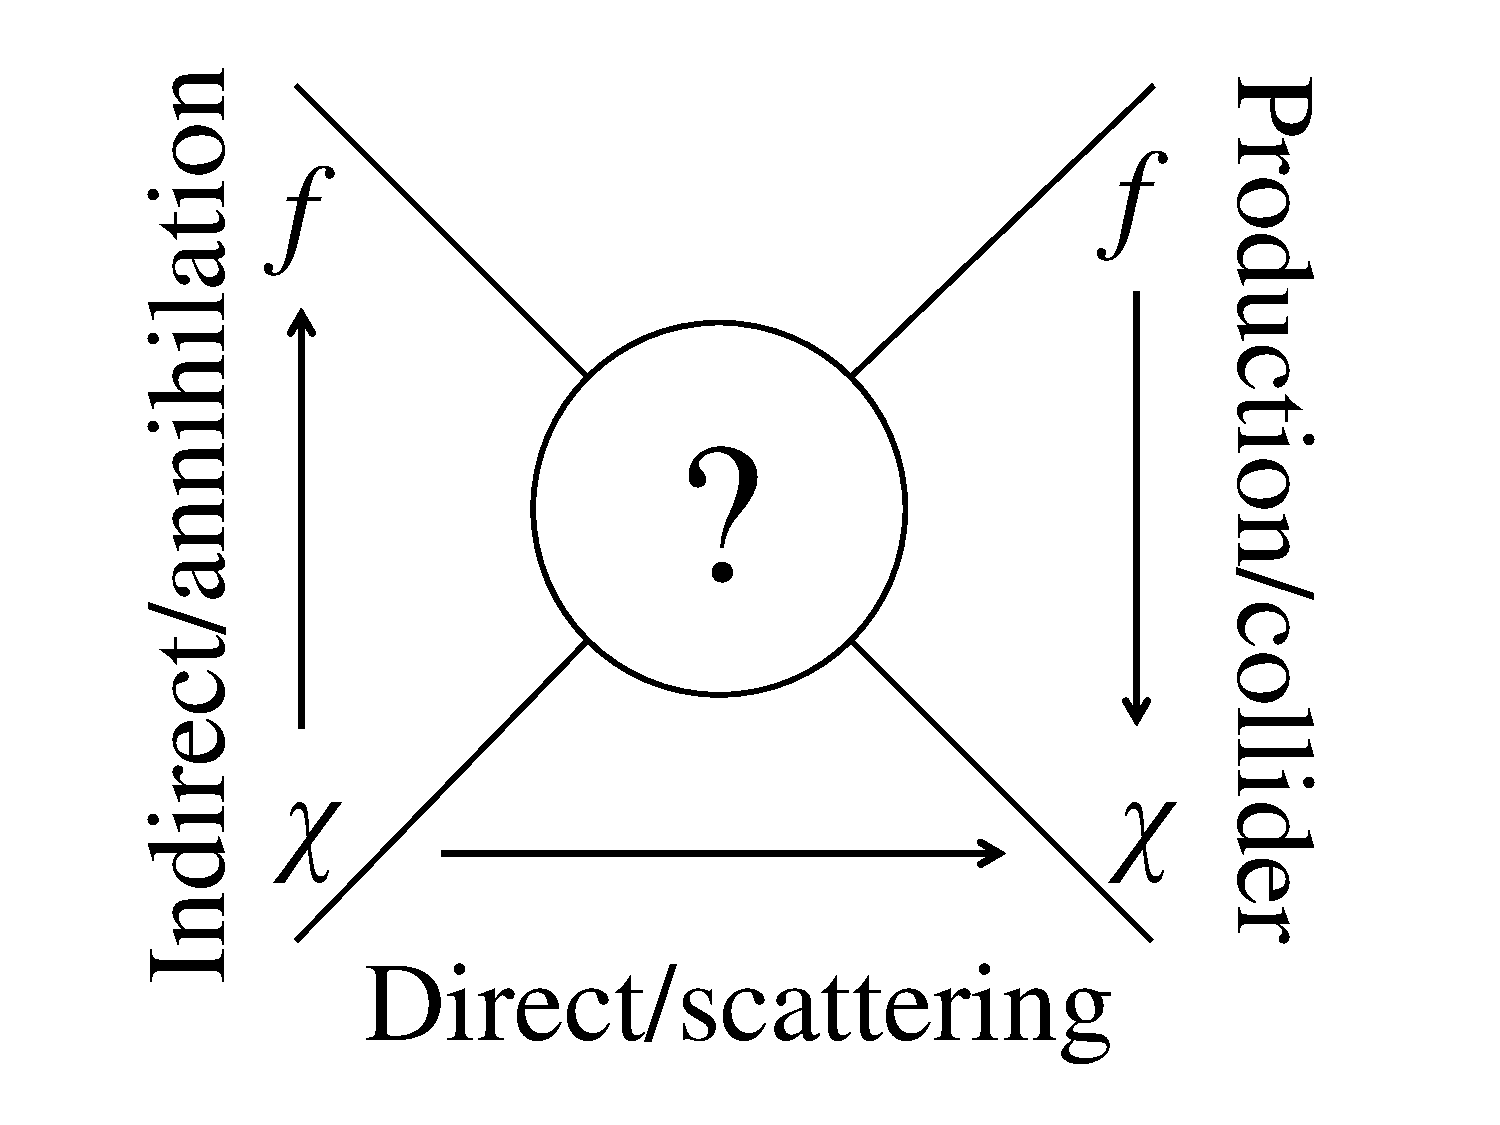
\includegraphics[width=0.8\textwidth]{figures/dm/feynman_diag}
    \caption{A Feynman diagram showing possible interactions between a Standard Model fermion \textit{f} and a dark matter particle $\chi$, and three different search methodologies.}\label{fig:feynman}
\end{figure}

\subsection{Production Searches}

Attempts to produce dark matter at colliders are led by the CMS~\cite{cms:2008} and ATLAS~\cite{atlas:2008} experiments at the LHC, following the interaction along the right side of Figure~\ref{fig:feynman}. Various parameter spaces are searched for the signatures of new particles, for instance the Higgs boson~\cite{cms:2012,atlas:2012}. Because any dark matter particle produced in the collision between (for instance) two protons is not expected to interact with a detector before escaping, the experimental signature of such an event would be missing momentum. Several searches for this signature have been performed, but the results so far are consistent with Standard Model expectations~\cite{atlas:2016,cms:2017}.

\subsection{Annihilation Searches}

In a region with higher dark matter density, such as galactic centers, the probability increases for any two dark matter particles to have some interaction with each other. Following the left side of Figure~\ref{fig:feynman}, two dark matter particles that annihilate could create a pair of standard model particles, which a detector could observe. Many experiments are engaged in these searches, including AMS~\cite{Aguilar:2013} and Fermi-LAT~\cite{Ackermann:2013uma} in space, and HESS~\cite{Abramowski:2014tra}, VERITAS~\cite{Arlen:2012}, and MAGIC~\cite{Aleksic:2013xea} on land, to name but a few. While occasional signals are seen at some significance, such as the $3.5\1{keV}$ line observed in 2014~\cite{Boyarsky:2014jta,Bulbul:2014sua}, astrophysical sources have been proposed and a concensus on the origin of these signals has not been reached~\cite{Shah:2016efh,Ahnen:2016qkx,Abdallah:2016ygi,Archambault:2017wyh,Albert:2016uux}.

\subsection{Scattering Searches}

The final interaction to discuss is the bottom of Figure~\ref{fig:feynman}. Here, a dark matter particle scatters off a target particle, imparting some momentum to the target. The three types of signals from these interactions are phonons, photons, and electron/hole pairs. Most detectors are designed to collect two of these three, leading to a wide variety of detector materials, designs, and configuration. These include crystals and bolometers, both semiconducting and inorganic, (CDMS~\cite{Akerib:2005,Agnese:2015ywx}, CRESST~\cite{Kluck:2017hnn}, and EDELWEISS~\cite{Armengaud:2009hc,Armengaud:2017rzu}), bubble chambers with superheated liquids (PICO~\cite{Amole:2015pla,Amole:2017dex} and COUPP~\cite{Manuel:2016klm}), noble liquid scintillation counters (DEAP~\cite{Amaudruz:2017ibl,Amaudruz:2017ekt} with argon, XMASS~\cite{Abe:2013tc} with xenon), and dual-phase noble time projection chambers (TPCs) (DarkSide~\cite{Agnes:2014bvk,Agnes:2015ftt} and ArDM~\cite{Marchionni:2010fi,Calvo:2015uln,Calvo:2016hve} using argon, and XENON10~\cite{Angle:2007uj}, ZEPLIN~\cite{Akimov:2011tj}, XENON100~\cite{Aprile:2011dd,Aprile:2013doa}, LUX~\cite{Akerib:2013tjd}, PandaX-II~\cite{Cui:2017nnn}, and XENON1T~\cite{Aprile:2017aty} using xenon). The easier scalability of noble liquid detectors over crystals makes them the dominant technology, and they continue to push to greater sensitivities. In these direct detection experiments, the usual parameter space to report results is that of the WIMP-nucleon scattering cross section versus the WIMP mass, as shown in Figure~\ref{fig:limits}. As no verified signals have been observed, experiments continue to place upper limits on in this space. We will focus on XENON1T, but much of this discussion applies to all direct detection experiments.

\begin{figure}[htb]
    \centering
    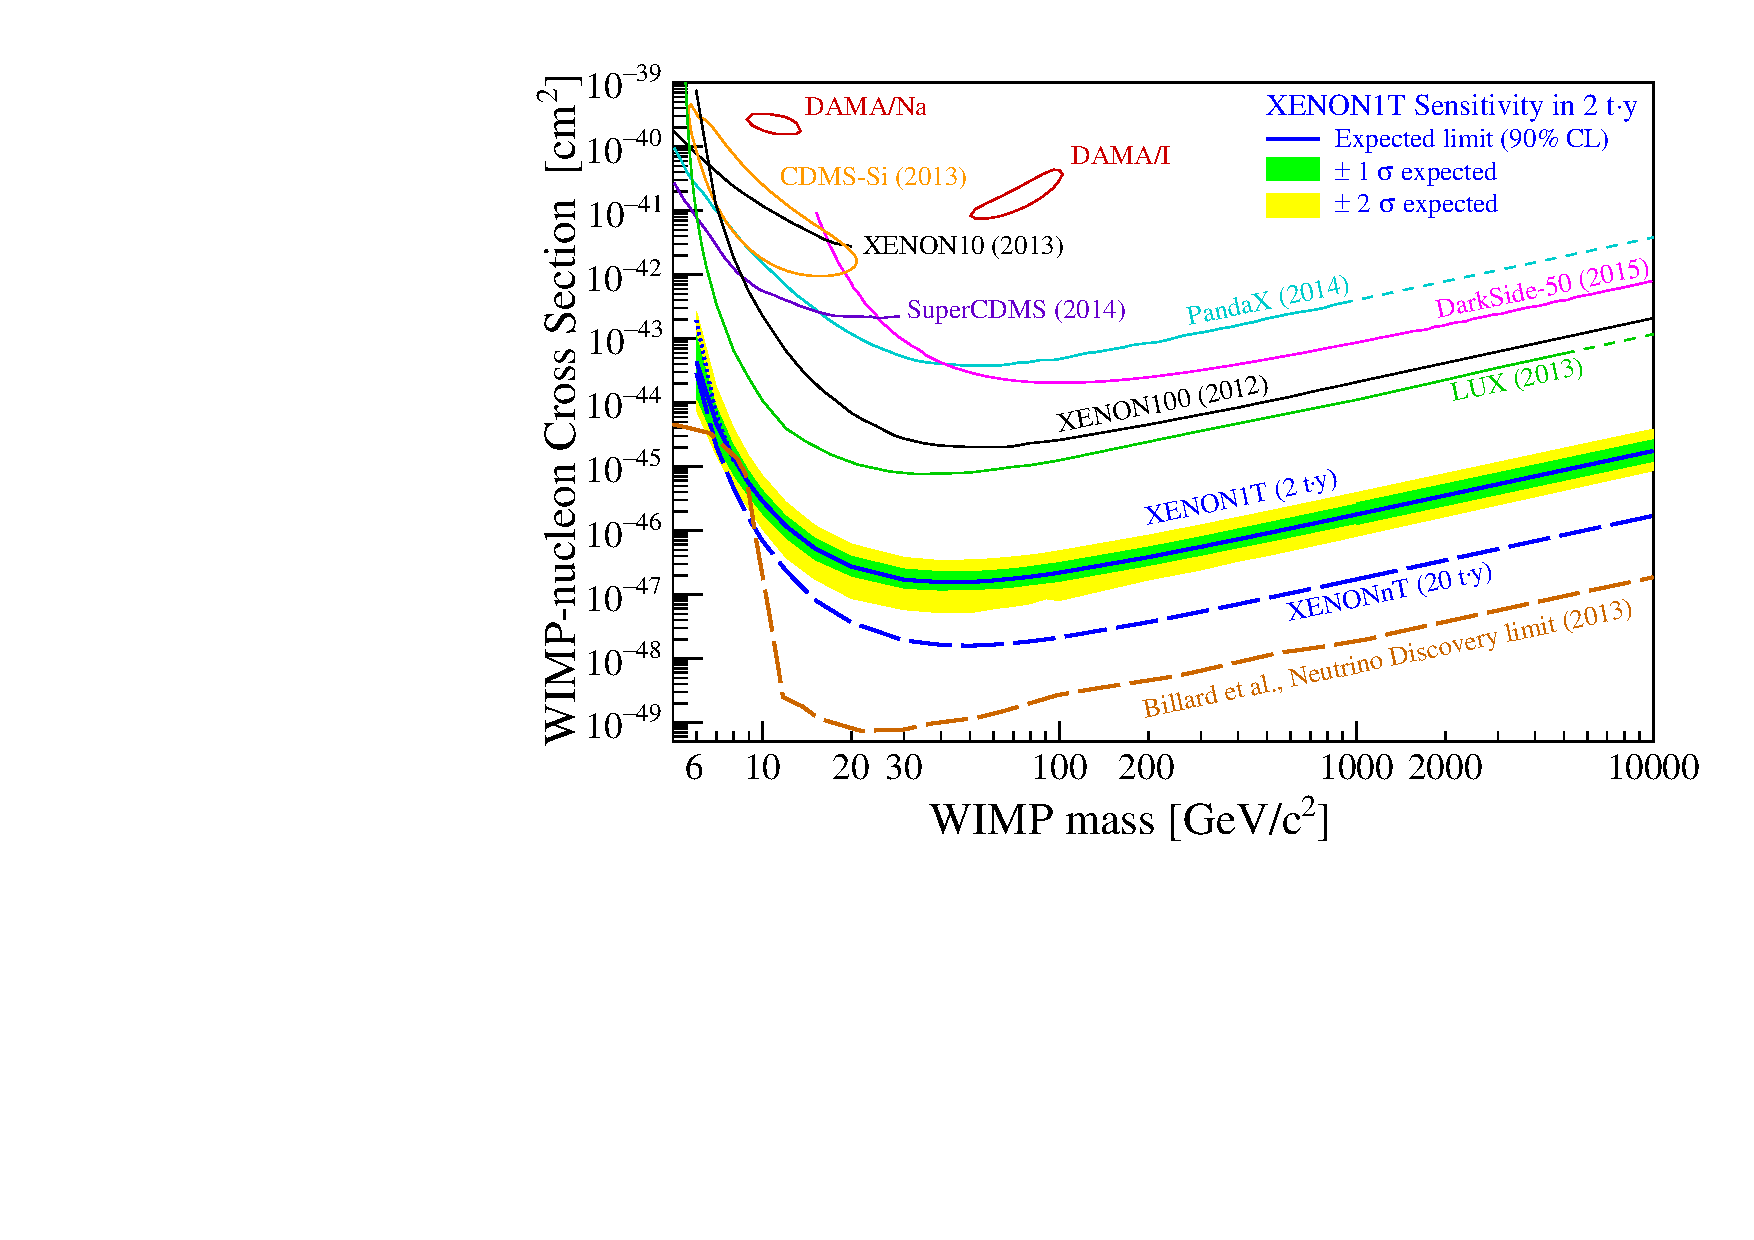
\includegraphics[width=0.8\textwidth]{figures/dm/limit_plot}
    \caption{Expected sensitivity of XENON1T to the spin-independent WIMP-nucleon scattering cross section, from~\cite{Aprile:2015uzo}. Included are results and exclusion limits from DAMA-LIBRA~\cite{Savage:2008er}, CDMS-SI~\cite{Agnese:2013rvf}, XENON10~\cite{Angle:2013}, SuperCDMS~\cite{Agnese:2014aze}, PandaX~\cite{Xiao:2014}, DarkSide-50~\cite{Agnes:2015ftt}, XENON100~\cite{Aprile:2012nq}, and LUX~\cite{Akerib:2015rjg}. The background due to coherent neutrino-nuclear scattering is from~\cite{Billard:2013qya}. The scalability of liquid noble detectors, especially those using xenon, have significantly outpaced semiconductors above a dark matter mass of a few GeV. Also shown is the projected sensitivity for the XENONnT detector upgrade. The decrease of sensitivity to lower mass dark matter arises from the reduced energy deposition in an interaction and the difficulty of detecting these smaller signals; the decrease towards higher mass is due to the decreasing dark matter number density and flux.}\label{fig:limits}
\end{figure}

Additionally, given the focus of this thesis, there are a number of other topics relevant to our discussion of direct detection experiments, such as backgrounds and the specifics of the expected signals.

\subsubsection{Backgrounds}

The limiting factor of any experiment is the background to the signal of interest. As the expected signature of a WIMP interaction is a low-energy nuclear recoil (NR), any process that also produces this is a potential background. Sources of neutrons, then, are especially dangerous. The three dominant sources of neutrons and nuclear recoil events for XENON1T are radiogenic and cosmogenic neutrons, and coherent elastic neutrino-nuclear scattering (CEvNS)~\cite{Freedman:1977,Scholberg:2015,Billard:2013qya}. Radiogenic neutrons are due to the $(\alpha,n)$ reaction and spontaneous fission of uranium and thorium contaminants in detector materials; cosmogenic neutrons are caused by muon-induced spallation; CEvNS events are primarily due to neutrinos produced by $^8$B in the solar core. Taken together, the expected nuclear recoil background rate in the range (4,~50) $\n{keV}_{nr}$ in XENON1T is $(0.6 \pm 0.1)\1{(tonne\cdot y)^{-1}}$~\cite{Aprile:2015uzo}, predominantly from the radiogenic neutrons. Below 3~$\n{keV}_{nr}$ the rate from CEvNS increases significantly, rising to $\sim 90\1{(tonne\cdot y)^{-1}}$ at a 1~keV threshold.

Additionally, there are backgrounds rising from electronic recoils (ER) that leak into the nuclear recoil region of interest. Because the discrimination between electronic and nuclear recoils for most detectors is merely good and not perfect, an ER rejection level of $99.5\%$ means $0.5\%$ of ER events will leak into the NR band. The major sources of ER events are low-energy $\beta$ decays of \Pb~(one of the daughters of \Rn) and $^{85}$Kr, solar neutrinos from the $pp$ process that scatter off electrons, Compton scatters from $\gamma$s emitted by contaminants in the materials, and low-energy $2\nu\beta\beta$ decays of $^{136}$Xe, as shown in Figure~\ref{fig:er_bkg}.

\begin{figure}[htb]
\centering
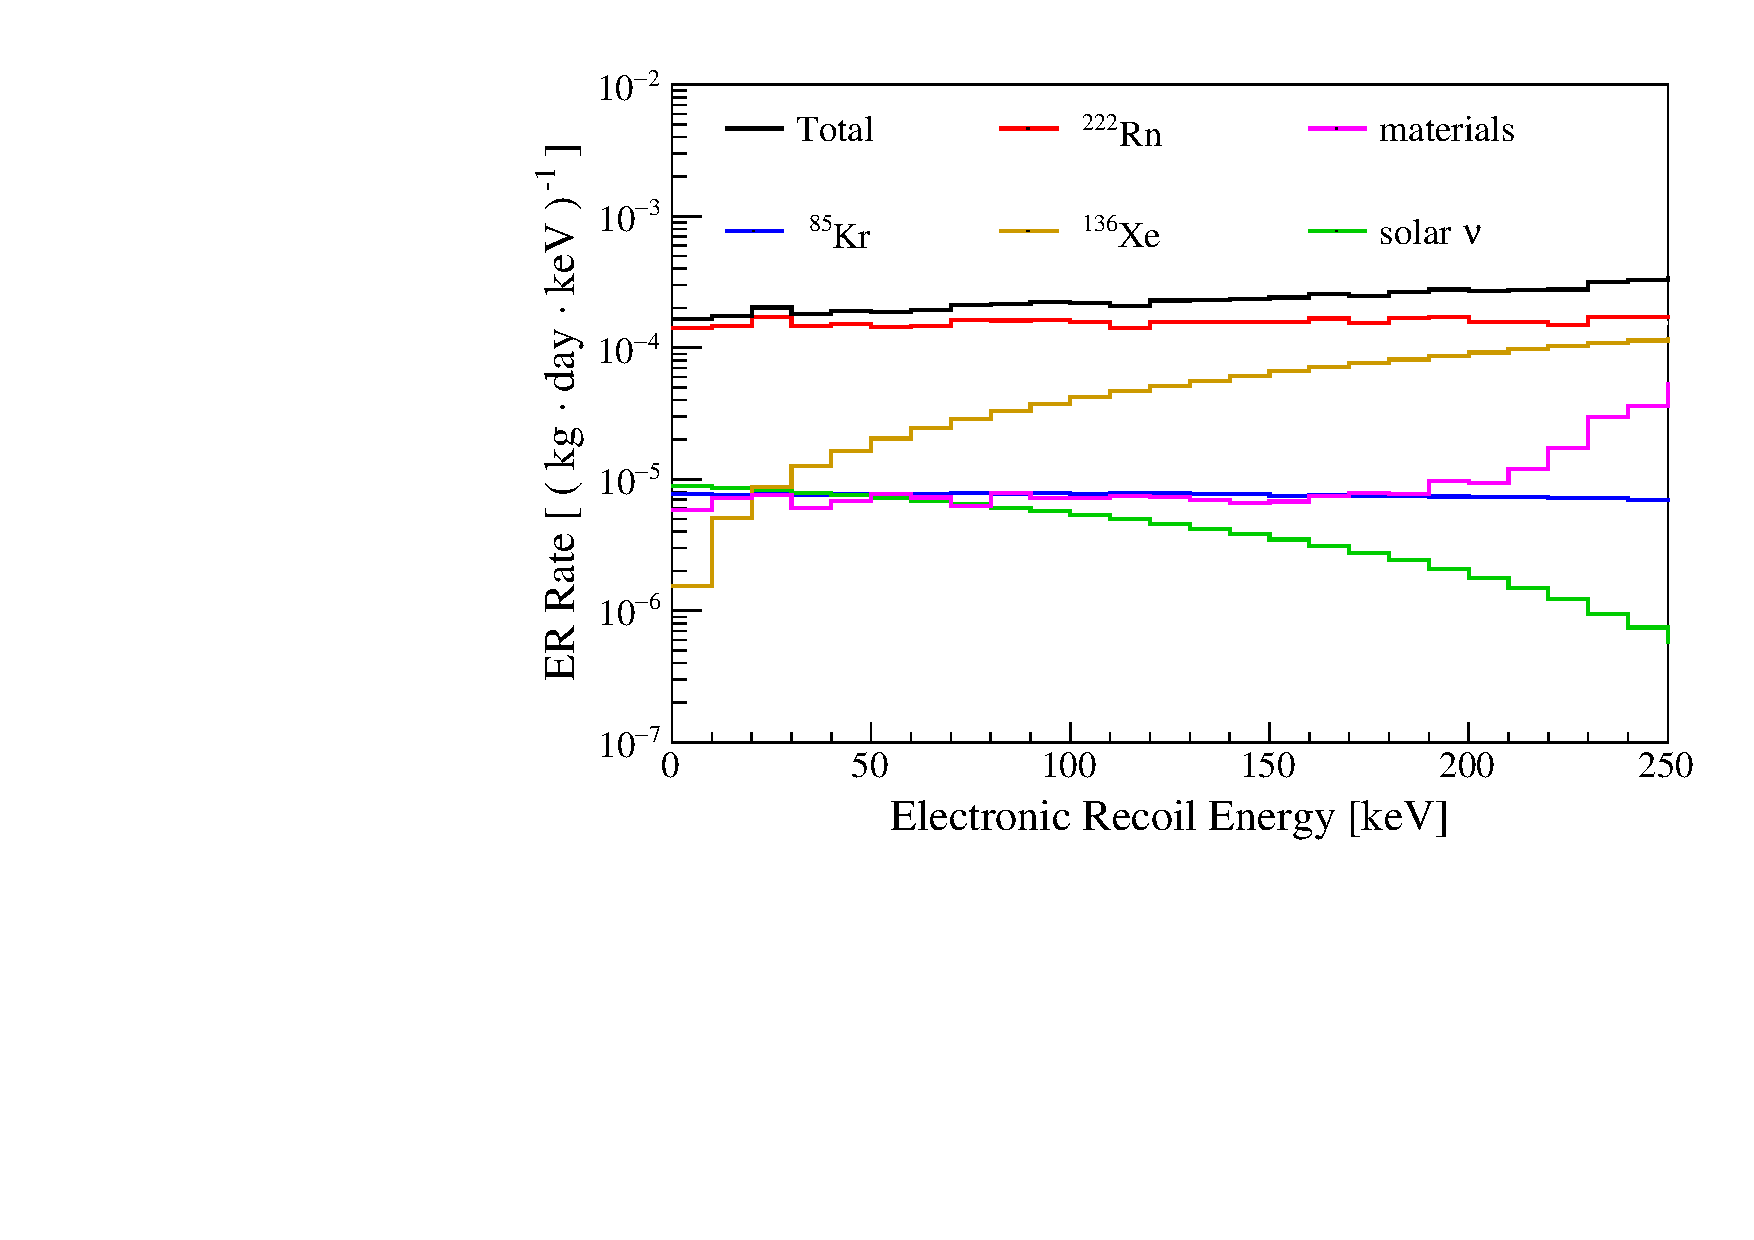
\includegraphics[width=0.8\textwidth]{figures/dm/er_bkg_low}
\caption{The simulated low-energy electronic recoil background spectrum in the XENON1T fiducial volume. The energy region of interest for dark matter events is the first bin. The concentration of \Rn~is $10\1{\mu Bq/kg}$ and of Kr is $<0.2\1{ppt}$. The $^{136}$Xe abundance is assumed to be natural. Figure from~\cite{Aprile:2015uzo}.}\label{fig:er_bkg}
\end{figure}

The background from krypton can be mitigated by removing krypton through cryogenic distillation~\cite{Aprile:2016xhi} and the backgrounds from \Rn~and material components by careful material screening and selection~\cite{Aprile:2017ilq}. $^{136}$Xe can be removed by the depletion/enrichment processes used commonly for nuclear power. Neutrino backgrounds are impossible to shield against or reduce, and represent fundamental limitations to the search for dark matter. The assumed values for XENON1T are a \Rn~concentration of $10\1{\mu Bq/kg}$ and Kr of $<0.2\1{ppt}$ (of which the $^{85}$Kr abundance is $2\times10^{-11}$), as given in~\cite{Aprile:2015uzo}. This gives XENON1T the lowest background rate of any dark matter experiment of $0.1\1{counts~(keV\cdot tonne\cdot day)^{-1}}$.

\subsubsection{Energy spectrum}

To calculate the expected spectrum of energy deposited in a detector, we combine information about the density $\rho_0$ and velocity distribution $f(v,t)$ of galactic dark matter, the differential scattering cross-section $\dd\sigma/\dd E(E,v)$, and the mass of the target and dark matter particles $m_A$ and $m_{\chi}$, respectively, as described in (for example)~\cite{Undagoitia:2015gya,Lewin:1996}:
\begin{equation}\label{eq:recoil_spectrum}
\frac{\dd R}{\dd E}(E,t) = \frac{\rho_0}{m_A \cdot m_{\chi}} \int\dd^3v\,v\,f(v,t)\frac{\dd\sigma}{\dd E}(E,v)
\end{equation}

The time dependence of equation~\eqref{eq:recoil_spectrum} arises due to the motion of the earth around the sun (and, to a much lesser extent, of a detector around the earth).

In general, the differential scattering cross-section can be expressed as a combination of spin-independent and spin-dependent components,
\begin{equation}\label{eq:si_sd}
\frac{\dd\sigma}{\dd E} = \frac{m_A}{2\mu_{A}^2v^2}(\sigma_0^{\n{SI}}F^2_{\n{SI}}(E) + \sigma_0^{\n{SD}}F^2_{\n{SD}}(E))
\end{equation}
where $\mu_A$ is the reduced mass of the dark matter and target particle and $F_i$ is the spin-dependent or -independent form factors. Figure~\ref{fig:dm_rate} shows the expected differential rate for a spin-independent cross-section of $10^{-45}\1{cm^2}$ for a variety of different materials, WIMPs of mass $25$ or $100\1{GeV/c^2}$, and with and without the form-factor correction.

\begin{figure}[htb]
    \begin{tabular}{cc}
    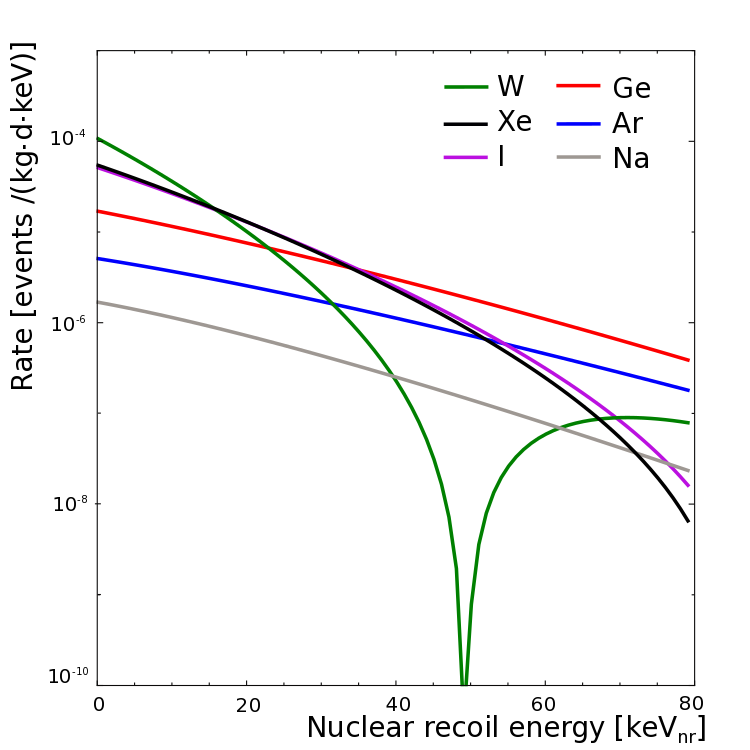
\includegraphics[width=0.4\textwidth]{figures/dm/rate_comp_v03} & 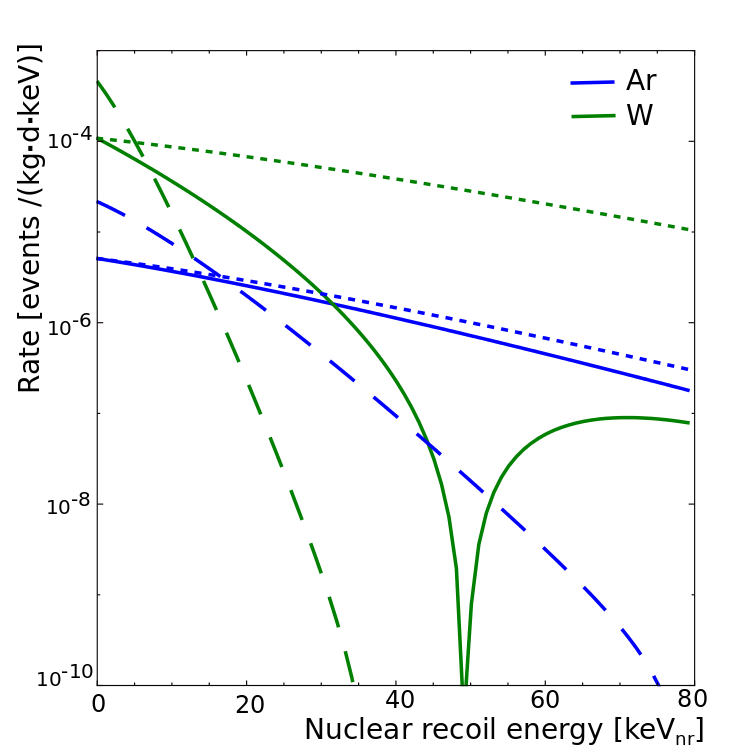
\includegraphics[width=0.4\textwidth]{figures/dm/rate_var_vs01} \\
    \end{tabular}
    \caption{(Left) WIMP differential interaction rate for a particle of mass $100\1{GeV/c^2}$ and cross-section $10^{-45}\1{cm^2}$ for a variety of different target materials. (Right) Reducing the WIMP mass to $25\1{GeV/c^2}$ yields the dashed lines, and neglecting the form factor yields the dotted lines. Figures from~\cite{Undagoitia:2015gya}.}~\label{fig:dm_rate}
\end{figure}

Reducing the mass of the dark matter particle increases the number density (as the energy density is fixed) and consequently the flux of particles through the detector, but as the particle velocity is constrained lower mass means lower energy, which in turn means less energy deposited in the detector. Likewise, increasing the dark matter mass reduces the flux but means the particles have higher energies.

\subsubsection{Annual modulation}

As the earth orbits around the sun, the sun in turn orbits the galactic center. In June, the velocities of the earth and sun are aligned, and in December they are antialigned. Thus, during June the flux of dark matter particles through a detector is slightly larger and in December is slightly less. Following~\cite{Freese:2012xd}, we express the energy spectrum as a Fourier series, of which the first two terms are
\begin{equation}\label{eq:modulation}
\frac{dR}{dE}(E,t) = S_0(E) + S_m(E)\cos (\omega t - \phi)
\end{equation}
where $S_0$ is the rate averaged over one year, $S_m$ the modulation amplitude (subject to $|S_m| \ll S_0$), $\omega = (2\pi)/(1~\n{year})$ the angular frequency, and $\phi$ the phase offset, set such that the rate has a maximum in June. Assuming that the detector operational stability is good for period of approximately one year or more, a modulation in the event rate can be measured and some potential dark matter interaction investigated~\cite{Aprile:2017yea,Abe:2018mxq}.

\paragraph{Conclusion} In this chapter we have investigated some of the evidence for the existence of dark matter, which constitutes much more of the universe than the protons and neutrons we are most familiar with. We discussed some detection strategies and results, and looked at some of the details of direct detection experiments, which will be the focus of this thesis.

% XENON1T
% xenon1t, v1.1

\chapter{The XENON1T Experiment}\label{ch:xe1t}

\paragraph{Abstract} This chapter provides an overview of the design and operation of the XENON1T detector and its associated subsystems. This is not an exhaustive treatment, instead focusing more on the wider picture than the equipment specifics, and the interested reader is recommended to Ref.~\cite{Aprile:2017aty} for a more complete description.

The XENON collaboration runs the world's leading WIMP direct detection experiment, and XENON1T is the third iteration in a series of ever-larger detectors~\cite{Angle:2007uj,Aprile:2011dd}. Built in central Italy at Laboratori Nazionali del Gran Sasso (LNGS), XENON1T is the largest and most sensitive xenon dual-phase time projection chamber (TPC) in the world at the time of commisioning, containing over $3200\1{kg}$ of xenon and a fiducial mass exceeding $1000\1{kg}$~\cite{Aprile:2017iyp}.

\section{Operational Overview}

The operation of the dual-phase TPC, such as the one employed by XENON1T, is as follows. When something interacts with a xenon atom inside the detector, it will produce excited atoms and liberated electrons. The excited atoms deexcite almost immediately, releasing photons that are collected by arrays of Hamamatsu R11410-21 photomultipler tubes (PMTs)~\cite{Aprile:2015lha} above and below the target. These photons provide what is called the \textit{S1} or \textit{prompt} signal. An external electric field drifts the electrons towards the liquid surface, where a second, much stronger field accelerates the electrons into the gas. These energetic electrons interact with the gas, creating more light that is again collected by the PMT arrays. This signal is variably called the \textit{S2}, \textit{delayed}, or \textit{ionization} signal. The time difference between the S1 and S2 is the amount of time the electrons were drifing, and yields the depth or $z$ coordinate of the interaction. The hit pattern on the top PMT array yields the $(x,y)$ position of the event, as the PMTs directly above the S2 location will see more photons and produce a stronger signal. Figure~\ref{fig:idealized_event} shows schematically a typical event.

\begin{figure}[htb]
\centering
	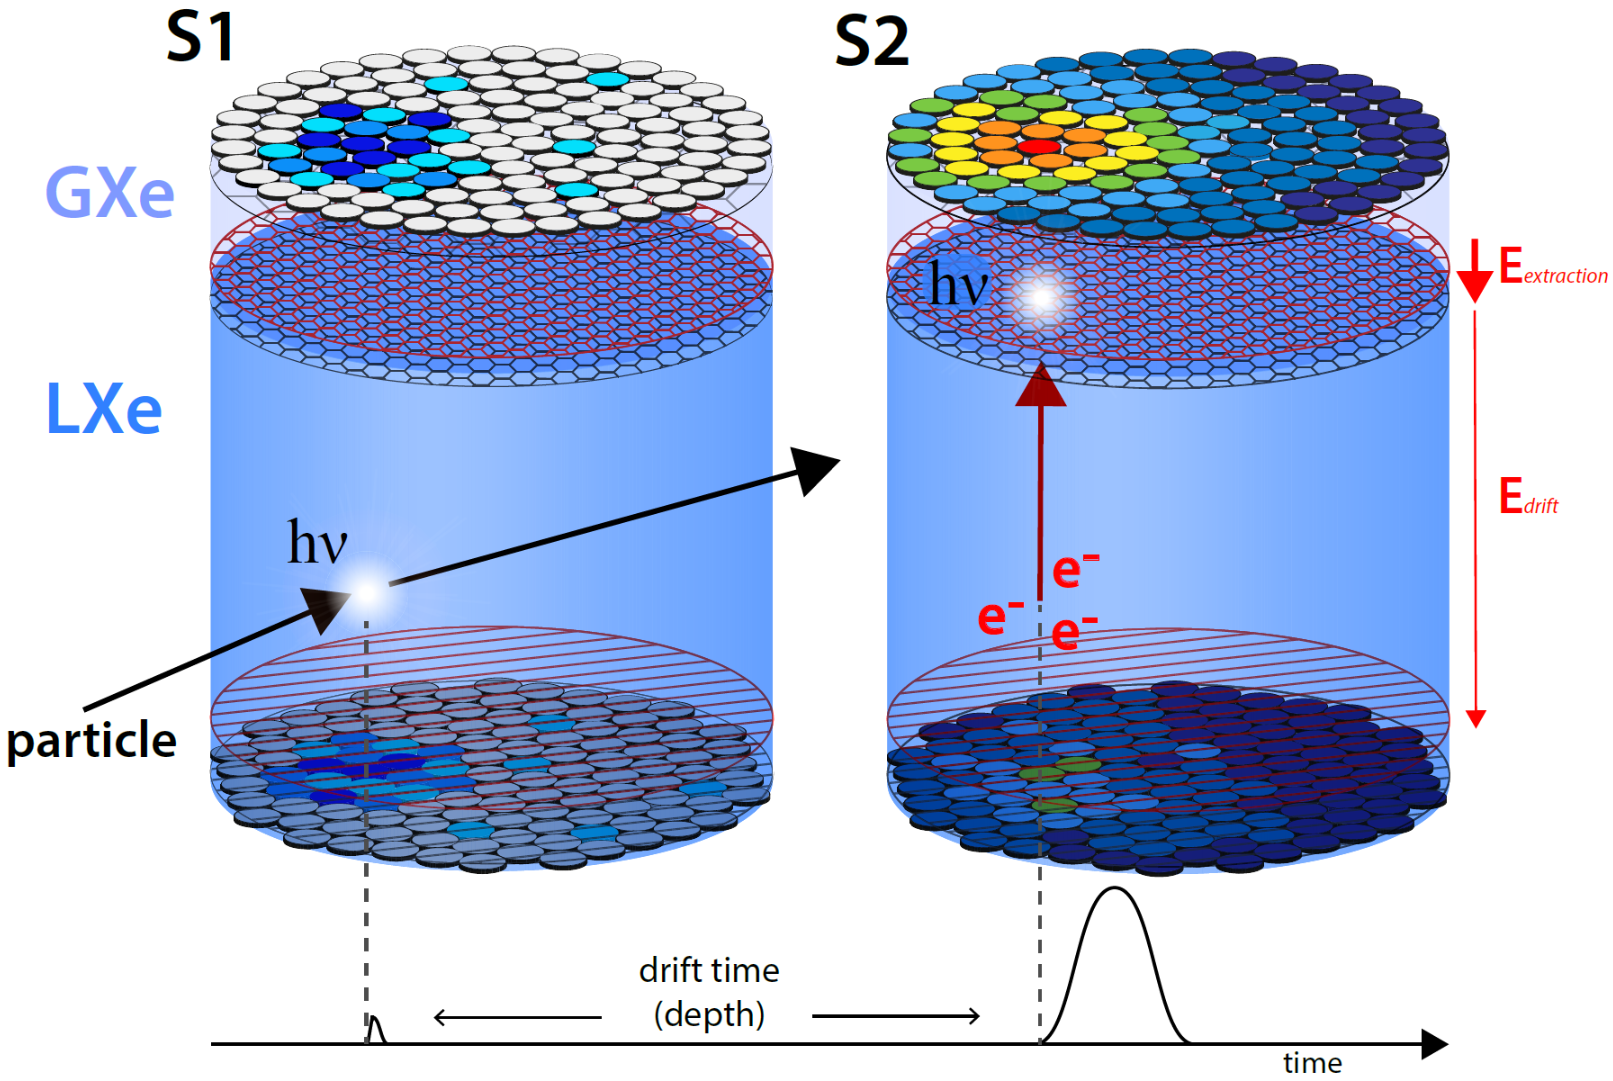
\includegraphics[width=0.8\textwidth]{figures/xe1t/tpc_xe1t_workingprinciple_v2.png}
	\caption{An idealized event inside a dual-phase TPC. An interaction in the liquid produces both prompt scintillation (\textit{S1}) and quasi-free electrons. Under the influence of an applied electric field, these electrons drift toward the liquid surface, where a second, stronger electric field extracts the electrons into the gas. These cause energetic collisions with the gasseous atoms, resuling in delayed scintillation (\textit{S2}). The time difference between signals indicates the depth of the interaction, while the hit pattern on the top PMTs indicates the transverse location.}\label{fig:idealized_event}
\end{figure}

The ability to reconstruct the position of an interaction in three dimensions yields the powerful ability of fiducialization. Additionally, xenon is very optically dense to high-energy photons. Because a significant source of background originates from materials surrounding the xenon, the combination of this self-shielding and the ability to determine where interactions occur allow us to define a fiducial volume where backgrounds are minimized.

\section{System Overview}

The XENON1T detector is composed of numerous subsystems to perform xenon handling, calibration, shielding, and data aquisition, and will be discussed here in some detail.

\subsection{Water tank}

The detector is housed in the center of a large tank of high-purity water, $10\1{m}$ in diameter and $10\1{m}$ in height. The rock overburden at LNGS reduces the cosmogenic muon flux to about 1 per square meter per hour~\cite{Bellini:2012te}, so muons will still regularly traverse the detector volume. However, by surrounding the detector with water, the Cherenkov radiation produced when muons (or particles from the showers they create) traverse this can be detected by an array of PMTs, and any coincident event in the TPC can be tagged~\cite{Aprile:2014zvw}.

Furthermore, the water also acts to shield the TPC from radioactivity in the surrounding rock. The trigger rate in the detector decreases significantly as the tank is filled, as shown in Figure~\ref{fig:waterlevel}.

\begin{figure}[htb]
    \begin{center}
    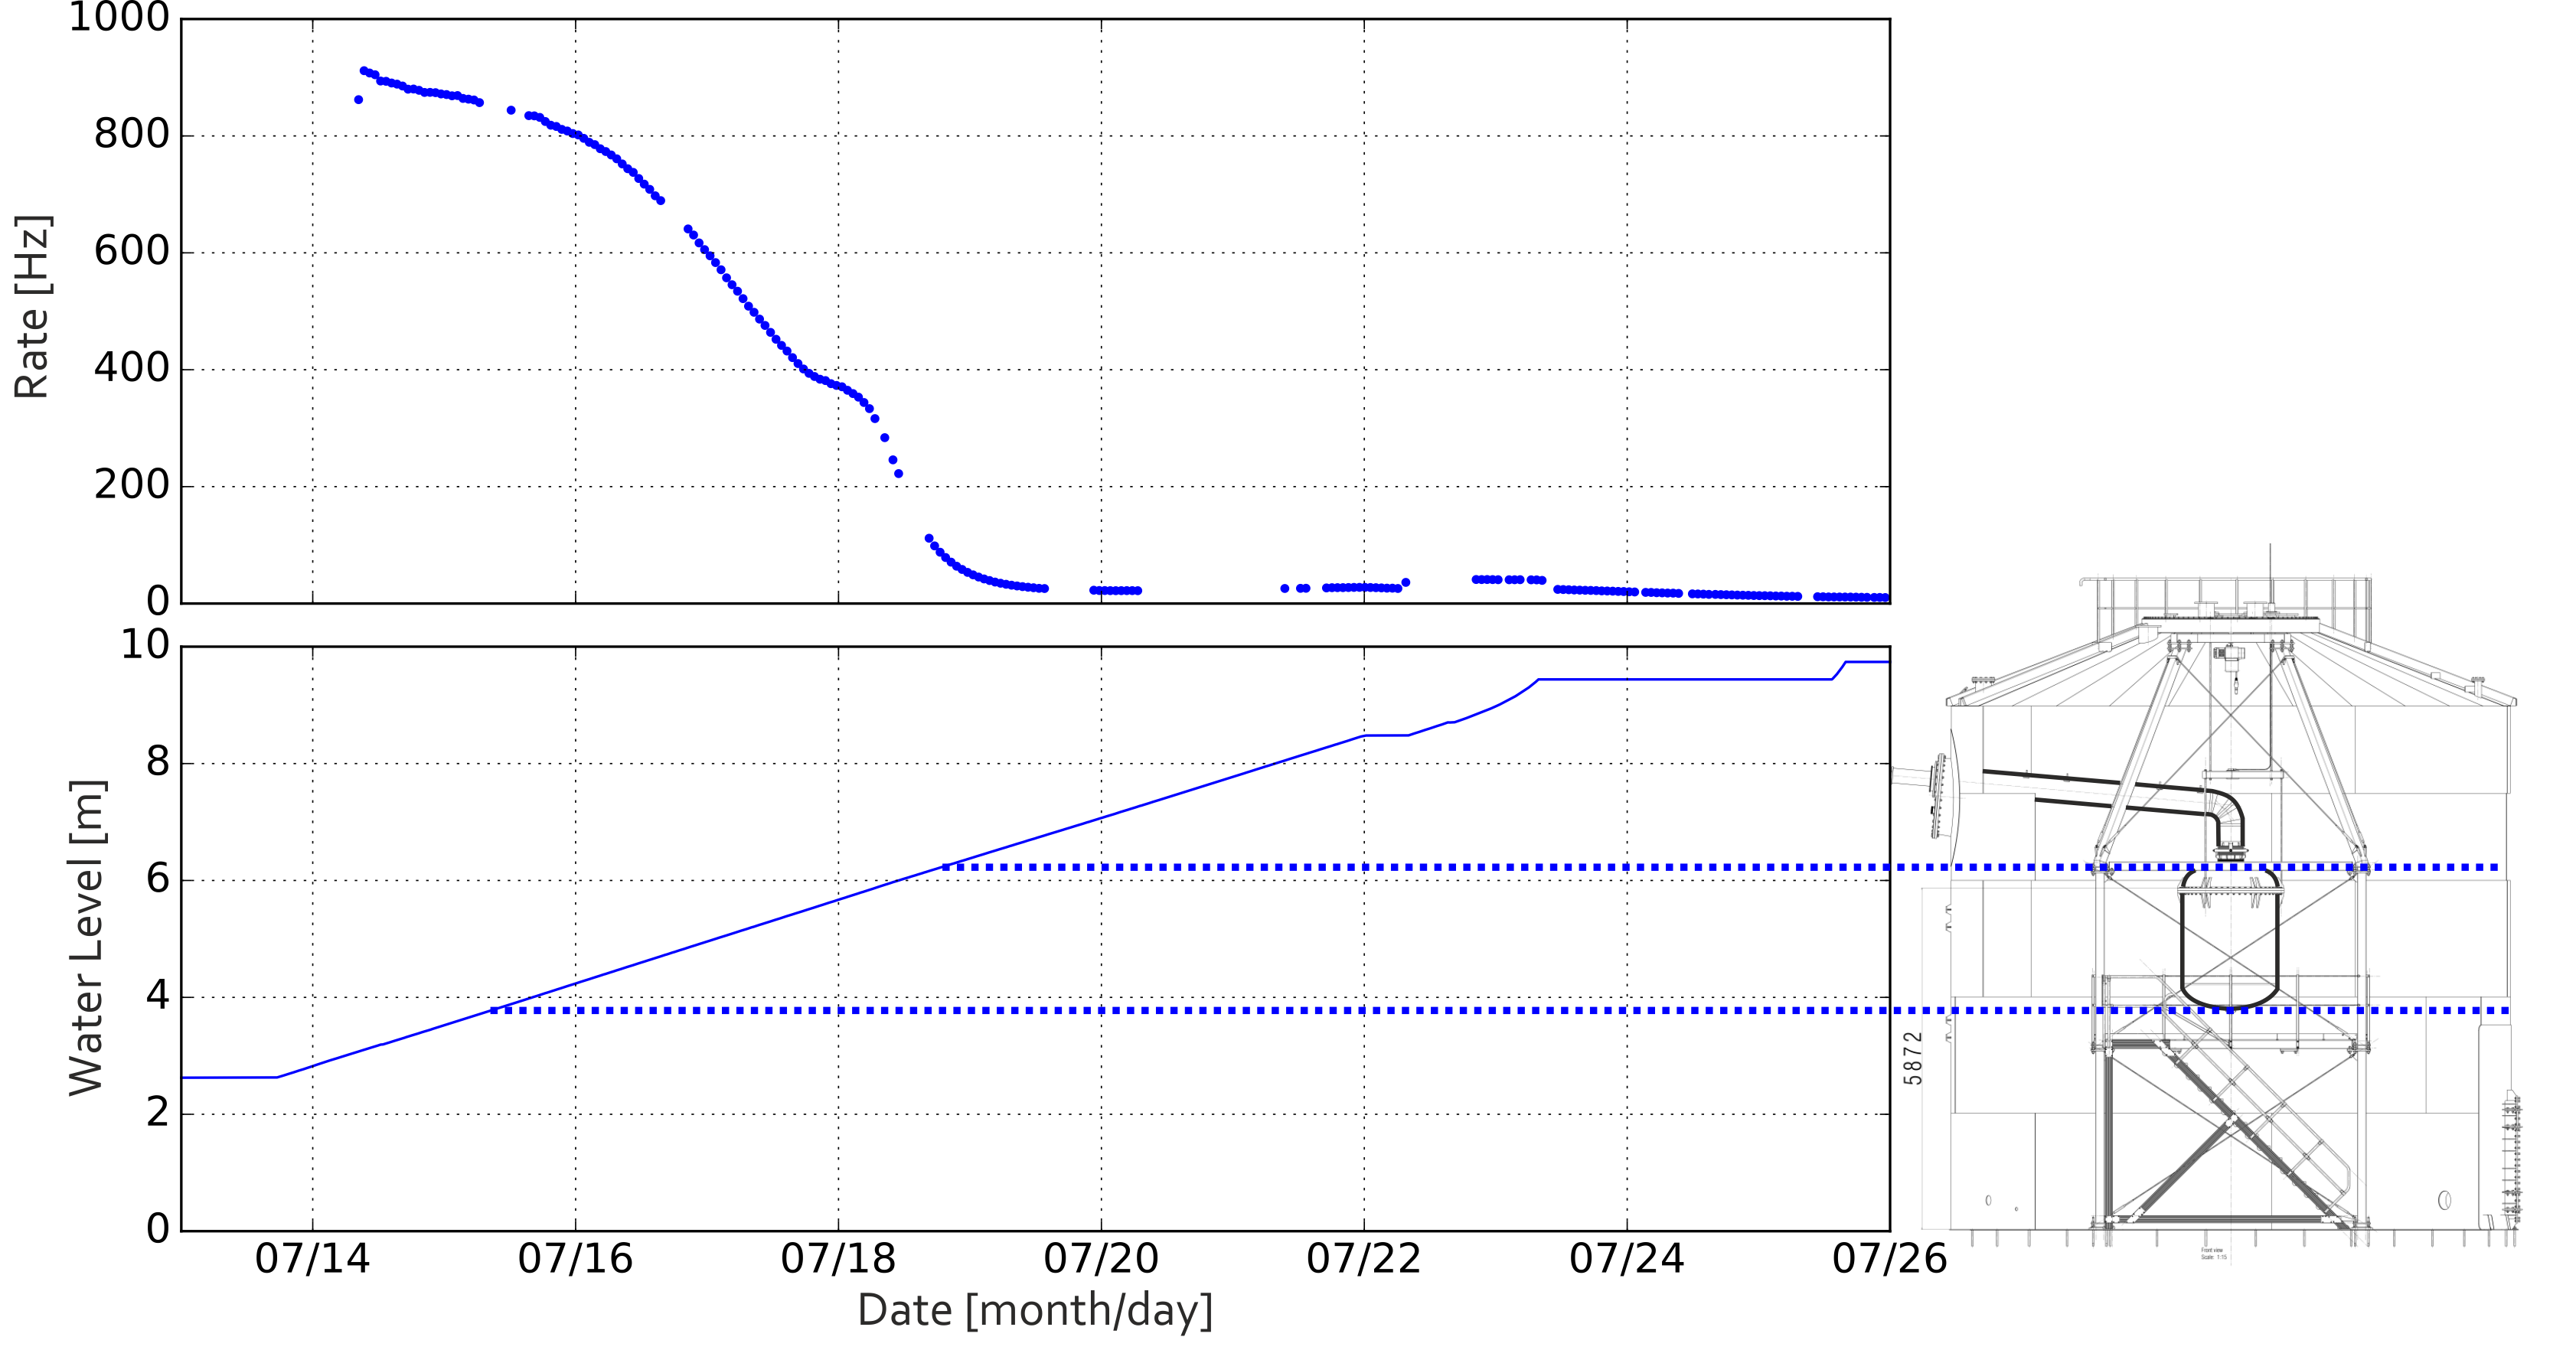
\includegraphics[width=0.8\textwidth]{figures/xe1t/water_level_part_2}
    \end{center}
    \caption{The trigger rate in XENON1T during the filling of the water tank. Surrounding the detector with several meters of water provides a reduction in trigger rate by two orders of magnitude.}\label{fig:waterlevel}.
\end{figure}

In the center of the tank stands the support structure that holds the cryostat, as well as the temporary platform which can be erected for maintenance on the TPC, cryostat, or surrounding systems.

\subsection{External calibration systems}

XENON1T has two primary external calibration systems. The first is known as the belt systems, and provide the ability to position radioactive sources at various locations surrounding the cryostat. The second is the deuterium-deuterium plasma fusion neutron generator~\cite{Lang:2017ymt} (see also Chapter~\ref{ch:ng}).

\subsubsection{Belt systems}

Three systems of belts are mounted in the water tank. Two of these systems have purely vertical travel (I-belts), and the third is capable of moving a source all the way underneath the detector along a secant (U-belt). These are located as shown in Figure~\ref{fig:belts}. Tungsten collimators mounted to carts on each belt allow $\gamma$s to be emitted in cones that illuminate much of the active volume.

\begin{figure}[htb]
\centering
    \includegraphics[width=0.8\textwidth]{figures/xe1t/cryo_belts_ng_colored}
    \caption{Placement of external calibration systems around the XENON1T cryostat. The neutron generator (green) is used for nuclear recoil calibrations, while the I-belts (blue) and U-belt (red) allow for the positioning of $\gamma$ sources to measure (among other things) self-shielding and electrical field distortion. The neutron generator can also be placed in two other locations around the cryostat (not shown) to provide a more uniform calibration.}\label{fig:belts}
\end{figure}

Sources of $^{137}$Cs, $^{228}$Th, and $^{241}$AmBe have been successfully deployed in these systems. A lead slug was mounted with the $^{241}$AmBe source to reduce the flux of high-energy $\gamma$s.

\subsubsection{Neutron generator}

While the increased size of XENON1T poses new challenges for calibration, it also offers new opportunities. The detector diameter is much larger than the mean free path of fast neutrons, so accurate reconstruction of multiple interaction vertices is possible. The energy deposited in an elastic interaction with a xenon nucleus is given by equation~\eqref{eq:doublescatter}.

\begin{equation}
\frac{E_{Xe}}{E_n} = \frac{2\frac{m_{Xe}}{m_n}(1-\cos\theta)}{\left(1+\frac{m_{Xe}}{m_n}\right)^2}
\label{eq:doublescatter}
\end{equation}

If the incident neutron energy $E_n$ is known, the deposited energy $E_{Xe}$ can be accurately measured. The masses of xenon and the neutron are $m_{Xe}$ and $m_n$, respectively, and $\theta$ is the scattering angle. By placing the neutron generator in a well-defined position next to the cryostat, the location of the neutron source is then known and accurate reconstruction of the scattering angle is possible.

A fast neutron travels at approximately $0.05\1{c}$, so will cross the detector in about $70\1{ns}$. While the temporal resolution is insufficient to resolve multiple S1s that occur in this time, the following S2 signals can be separated by tens or hundreds of microseconds. This is sufficient to perform accurate \textit{in situ} charge yield measurements, as demonstrated by LUX~\cite{Akerib:2016mzi}.

\subsection{Gas recirculation, purification, and cryogenics}

A large series of tubes and pipes exists to support the operation of the detector. This system is responsible for filling and emptying the detector, introducing radioactive sources into the detector for various calibrations, and maintaining the purity of the xenon in the detector by recirculating through hot zirconium getters. Two separate parallel lines, each containing pumps and a getter, provide increased xenon throughput as well as some redundancy in the event of maintenance requirements. A source box containing various internal calibration sources (including $^{83m}$Kr~\cite{Kastens:2010,Akerib:2017eql}, $^{220}$Rn~\cite{Aprile:2016pmc,Lang:2016zde}, and $\n{CH}_3\n{T}$~\cite{Akerib:2015wdi}) is connected to the gas system and allows the injection of sources both before and after the getters.

The paradigm for cooling is the same ``remote cooling'' configuration as was used in XENON100~\cite{Aprile:2011dd}. In this setup, cooling is provided by pulse tube refrigerators (PTRs) installed some distance from the TPC itself. Xenon gas from around the TPC diffuses upwards to the coldfingers, and the liquid xenon that condenses onto the colfingers flows back down pipes towards the TPC. This allows for easy maintenance of the cooling systems with only marginal impact on the system operation. Two redunandant PTRs, each rated for $250\1{W}$ of cooling at $177\1{K}$, are more than sufficient to provide the $\approx 150\1{W}$ of cooling necessary for stable operation. In the event of power loss or some other thermodynamic anomaly (for instance, failure of the insulation vacuum), backup liquid nitrogen cooling can maintain the system pressure at safe levels.

While electronegative impurities that emanate from materials are efficiently removed by the getters, noble element contaminants, such as krypton or argon, are not. One of these is the $\beta^-$ emitter $^{85}$Kr. Decays of this isotope contribute to the low-energy electronic recoil background and can be removed by cryogenic distillation, exploiting the different vapor pressures of xenon and krypton. A distillation column was constructed for this purpose, and successfully reduced the krypton level to the required $<0.2\1{ppt}$~\cite{Aprile:2015uzo,Aprile:2016xhi}. As krypton and argon are not produced in appreciable quantities once the xenon is safely underground, this purification only needs to be performed once. Additionally, the column can also be run in reverse mode to remove radon rather than krypton.

\subsection{Electronics and DAQ}

A variety of eletronics are housed in the service building adjacent to the water tank for the purpose of running the data acquisition (DAQ) systems. Each PMT requires connections for both signal and high voltage. PMT signals are fed through Phillips Scientific 776 amplifiers (providing a gain of 10) into CAEN V1724 ADC modules ($2.25\1{V}$ dynamic range, 14 bit resolution, $100\1{MHz}$ sample frequency) to digitize the traces. These are fed into a MongoDB noSQL database that acts as a circular buffer. Additionally, the waveforms for the top and bottom PMT arrays are summed and used to provide a high-energy veto. All signals with amplitude above $\sim 0.3\1{pe}$ are read asynchronously, zero-suppressed, and fed into the buffer database. Operating on this database is a program called the Event Builder, which monitors the data stream and saves any event-like patterns to disk. The criteria by which the Event Builder selects data is highly configurable, allowing for multiple trigger modes. Trigger metadata is also saved together with the waveforms. To allow for the measurement of small signals resulting from galactic supernovae neutrinos~\cite{Lang:2016zhv}, the untriggered data is stored for several hours after the end of a dark matter dataset, while the triggered data proceeds through the remainder of the computing chain. Upon receiving an alarm from the Supernova Early Warning System (SNEWS), the untriggered data can be saved and a dedicated analysis on this data can be performed.

The DAQ for the muon veto is nearly identical; the differences are a lack of the 10x amplification and the V1724 digitizers operating with $0.5\1{V}$ dynamic range. The trigger decision is made via a simple coincidence requirement. Waveforms are stored and recorded in the same database and in the same fashion as data from the TPC.

Data is buffered temporarily on the underground computing resources before being transferred above ground, where it is distributed for processing, tape backup, and analysis.

\subsubsection{Data processing}

Data processing is done by the PAX software~\cite{pax}, which operates in several steps. First, all pulses (zero-suppressed chunks of waveform) are scanned for \textit{hits}, which is any excursion from baseline. Hits are then clustered, based on the differences in time between them, to form \textit{peaks}. Peak properties are then calculated, including things like the area, width, and reconstructed $(x,y)$ position. Peaks are then classified as either S1, S2, or unknown, based on these properties. For instance, S1-like peaks tend to have fast rise-times and are seen more by the bottom PMTs, while S2-like peaks tend to be wider in time and seen more by the top PMTs. S1s and S2s are then grouped together to form \textit{interactions}, which is any valid pairing of an S1 and S2 (ie, the S2 must happen after the S1). This allows further information such as the drift time/$z$-coordinate to the calculated, and three-dimensional corrections to be applied, for instance for light collection efficiency, free electron absorbtion, and drift field distortion (giving \textit{cS1} and \textit{cS2}). The primary interaction used in data analysis is the pairing of the largest S2 in the waveform with the largest S1 preceeding it.

\subsection{TPC}

The TPC itself is housed inside the inner cryostat and is made of only the most radiopure materials available~\cite{Aprile:2017ilq}. The active region is surrounded by PTFE reflectors, copper rings to control the shape of the drift field, the PMT arrays, and the bell. A variety of tubes connect to the bell and run down to the region beneath the bottom PMT array to allow for the pressurization of the bell and recovery of xenon. The top and bottom PMT arrays contain 127 and 121 PMTs, respectively, for a total of 248. The bottom PMTs are packed as close as possible in a hexagonal fashion to improve light collection, while the top PMTs are arranged in a more radial fashion to improve position reconstruction. A picture of the arrays is shown in Figure~\ref{fig:pmt_arrays}. The drift region between the PMTs is $96\1{cm}$ in diameter and $97\1{cm}$ in height, which holds 2 tonnes of liquid xenon. A total of five electodes are installed: the cathode, the anode, two screening meshes to protect the PMTs from the strong fields near the cathode and anode, and the gate. The cathode and screening meshes are made from stretched wires, while the anode and gate are etched meshes.

\begin{figure}[htb]
\centering
    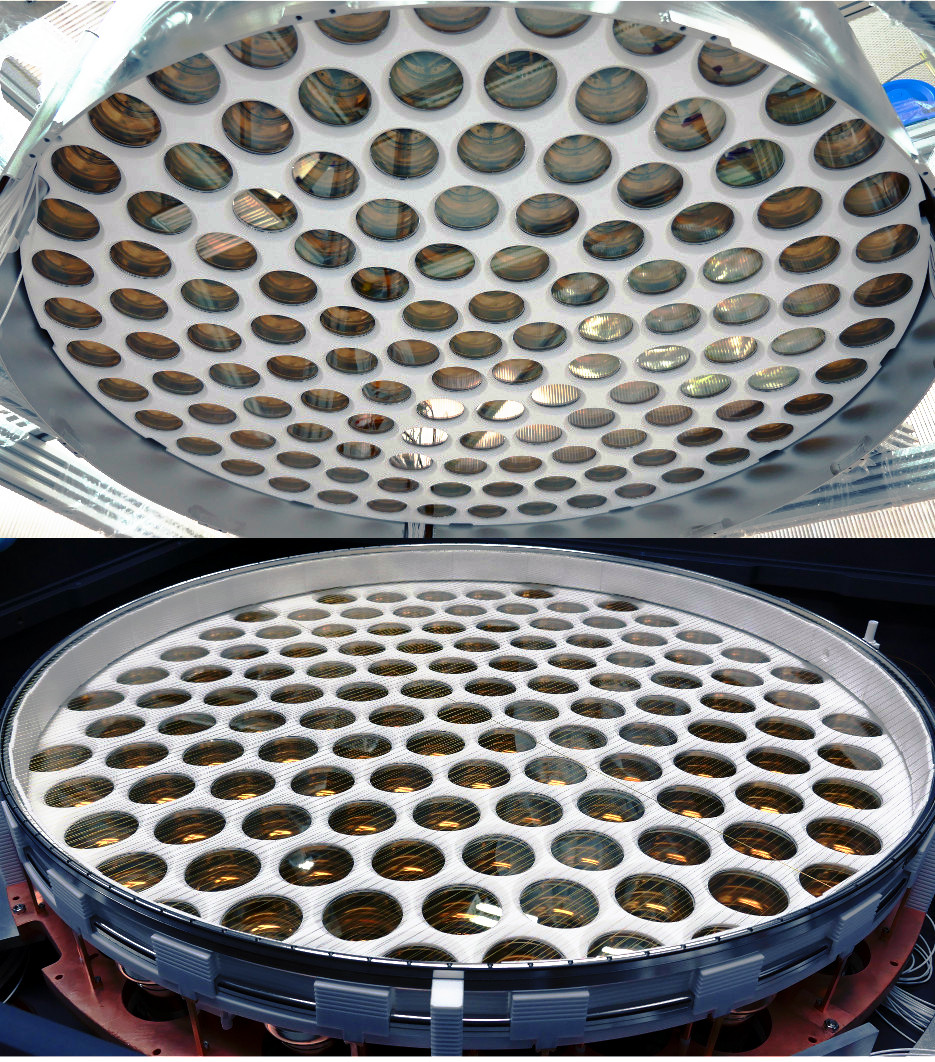
\includegraphics[width=0.8\textwidth]{figures/xe1t/pmt_arrays}
    \caption{A photograph of the arrays of Hamamatsu R11410 photomultiplier tubes in XENON1T. (Left) The top 127 PMTs are arranged to optimize position reconstruction, while (right) the bottom 121 are arranged to optimize light collection. The wires forming the cathode are just visible above the bottom PMTs.}\label{fig:pmt_arrays}
\end{figure}

To determine the height of the liquid both inside and outside the bell, six capacitive levelmeters are installed. Four short levelmeters (SLM) measure the height of the liquid between the gate and anode, while two long levelmeters (LLM) measure the liquid level outside the TPC. The LLMs employ a concentric cylinder construction, while the SLMs are formed from parallel plates.

The liquid level is set by pressurizing the bell through controlled xenon gas flow. The piping necessary for this, as well as the other pipes and cables for the PMTs, electrodes, and other sensors, all run through an umbillical pipe and out the side of the water tank.

\subsection{Summary}

The XENON1T experiment represents the pinnacle of liquid xenon TPC technology. With the lowest background yet achieved in the dark matter signal region of interest, XENON1T is the most sensitive dark matter detector ever constructed and will probe large portions of promising WIMP interaction parameter space. Further, the support subsystems were designed to easily accomodate an upgrade to the significantly larger XENONnT detector, with a target mass of approximately 6~tonnes. XENONnT is currently under construction and should begin commissioning in late 2018.

% psd paper
% PSD, v1.0

\chapter{PULSE SHAPE DISCRIMINATION IN LIQUID ORGANIC SCINTILLATORS}\label{ch:psd}

\paragraph{Abstract} To calibrate the response of XENON1T to nuclear recoils, we acquired a deuterium-deuterium plasma fusion neutron generator. Before deploying it on the world's most sensitive dark matter detector, it must be characterized (see Chapter~\ref{ch:ng}). To characterize it we must first understand the neutron detectors selected for this purpose, specifically, how to separate the neutron-induced signals from the backgrounds. The standard method of discriminating the nuclear recoil signals from the electronic recoil background in these detectors is via the shape of the pulse. In the liquid organic compounds popular for detection of fast neutrons, nuclear and electronic recoils excite molecules to states with different livetimes. A variety of algorithms, both new and well-known, were implemented for this purpose, and their performance measured, along with the energy dependence of this performance. The results have been published as Lang et al, Nuclear Instrumentation and Methods, A856:26-31 (2017) and are reproduced here.

\section{Introduction}

\begin{figure}[htbp]
\centering
    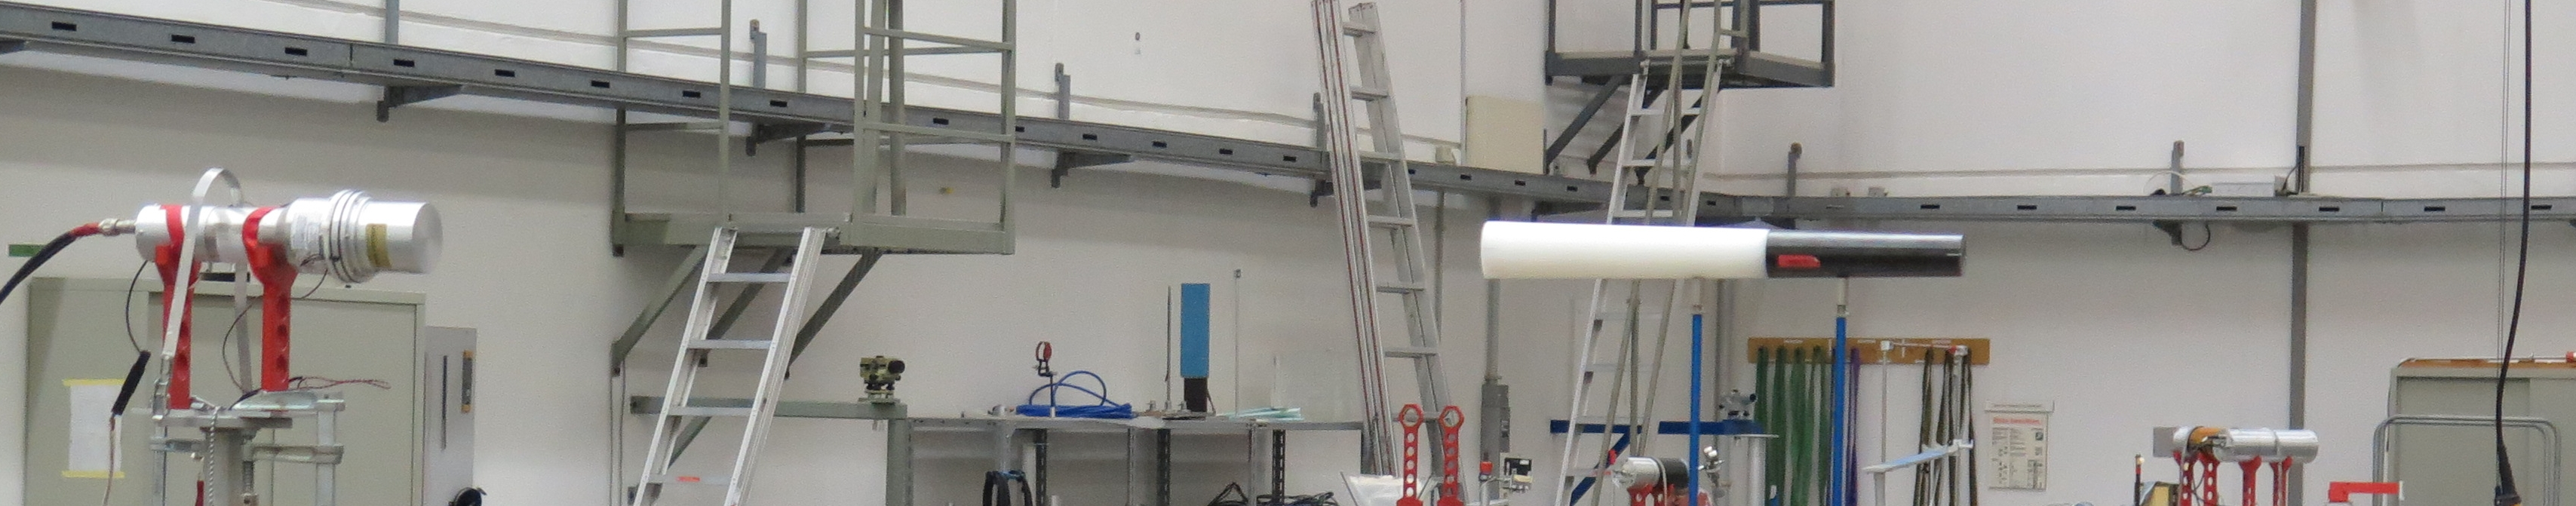
\includegraphics[width=\textwidth,height=4cm]{figures/psd/fig_ptb_setup}
    \caption{The irradiation setup of the EJ-301 detector (left) corresponding to the $0\degree$ orientation in Table~\ref{tab:psd_datasets}. The shadow cone is visible toward the right. The neutron beam enters the setup from the right.}\label{fig:psd_detector_setup}
\end{figure}

Liquid scintillators such as EJ-301 (which is similar to NE-213 and BC-501) are very popular for neutron detection as they can easily be shaped into the desired size and geometry of a given application and offer fast timing performance. However, since such liquid scintillators are also sensitive to gamma rays, pulse-shape discrimination (PSD) techniques are essential in order to correctly identify neutron interactions in the detector.

The ability to discriminate nuclear recoil (NR) events from electronic recoil (ER) events originates in the particular production mechanisms of scintillation light in organic liquid scintillators. These liquids are aromatic compounds which have planar molecular structures built up from benzenoid rings. Such structures allow for extended groupings of conjugated molecular bonds between unsaturated carbon atoms~\cite{Brooks:1979}. This results in some of the valence electrons of the carbon atoms being delocalized in $\pi$-molecular orbitals. It is the excitations of these $\pi$-electronic states that create the fluorescence observed in organic scintillators. During these excitations, $\pi$-electrons can be promoted from the ground state~S$_0$ to excited singlet states~S$_n$ or triplet~T$_n$ states. For low excitation densities, all excited singlet states above the first excited singlet states S$_1$ decay rapidly and non-radiatively to the lowest excited singlet state. This state then decays exponentially producing fluorescence in the process.

In contrast, the decay of the triplet state is governed by the diffusion time-scale of the triplet exciton and results in delayed fluorescence in which the intensity does not decay exponentially. NRs exhibit greater energy-loss rates and thus have higher densities of triplet states. Pulses from the ionization tracks of these particles exhibit higher yields of delayed fluorescence, hence decaying more slowly than those of ERs. Scintillation light from EJ-301 has three main decay components: $3.2\1{ns}$, $32\1{ns}$ and $270\1{ns}$~\cite{Kuchnir:1968}. The slowest of these decay times is produced by the delayed fluorescence of triplet states.

The different pulse shapes that arise from electronic and nuclear recoils in liquid scintillators can be exploited using different PSD techniques. The most popular techniques applied are the Charge Comparison Method~\cite{Brooks:1959} and the Zero Crossing Method~\cite{Alexander:1961}. These methods were originally implemented in purpose-designed analogue electronics~\cite{Adams:1978}, but with the advent of greater computing power at reduced costs, these techniques have been implemented digitally~\cite{Kaschuck:2005, Cester:2014, Liao:2014}. Digital capture of the full waveform allows for offline processing of events, reducing dead time in data acquisition systems. Techniques designed for analogue circuits do not take advantage of the increased information available in the digital domain. Consequently, new PSD techniques have been developed recently~\cite{DMellow:2007, Gamage:2011, Yousefi:2009}. These techniques offer new pulse shape discrimination approaches in the time domain of the waveform, allow frequency-domain and decay-time differences to be investigated using wavelet analysis, and can implement Fourier and Laplace transforms.

Traditionally, the performance of PSD techniques is characterized using the Figure of Merit (FOM), defined as:
\begin{equation}\label{eq:FOM}
\text{FOM} = \frac{\text{Peak Seperation}}{\text{FWHM}_\gamma+\text{FWHM}_n}
\end{equation}
where peak separation refers to the distance between the center of the neutron and gamma distributions in a histogram of the discrimination parameter, and $\text{FWHM}_i$ is the full-width half maximum of the respective distributions. Hence, the FOM does not provide any information on the energy dependence of the performance of PSD techniques. This precludes a comparison of the various algorithms across different authors that may use different energy thresholds in the calculation of their FOM, and additionally, may mask performance issues of the algorithms in particular at low recoil energy. Therefore, we examine the energy-dependent ability of PSD techniques to discriminate between electronic recoil and nuclear recoil events. Furthermore, we determine the efficiency of EJ-301 for detection of neutrons as a function of energy.

\section{Setup}

The fast neutron detector used in this work is a 3"~cell of EJ-301 liquid organic scintillator optically coupled to a fast photomultiplier tube (PMT), type 9821KB manufactured by ET Enterprises. The detector response to neutrons was characterized at the Physikalisch-Technische Bundesanstalt (PTB) in Braunschweig, Germany,  using a deuterium ion beam hitting a Ti($^3$H) target. The deuterium ion beam energy (3.356 MeV) was chosen to produce $(2.500\pm 0.010)\1{MeV}$ (k=1 according to~\cite{GUM}) monoenergetic neutrons via $^{3}$H(d,n)$^{4}$He nuclear reaction, in the direction of the ion beam. The detector was placed $3\1{m}$ from the target. The output of the PMT was connected to a CAEN DT5751 digitizer, which samples at 1~GHz with a resolution of 10~bits.

Data were collected at three different nominal beam current settings to study the effect of neutron flux on the performance of the detector. The detector was placed such that the angle between the direction of the ion beam and the normal of the front face of the detector was $0\degree$. The distance between the front face of the detector and the active layer of the target was $(3000\pm 2)\1{mm}$ (k=2~\cite{GUM}) for all measurements. Additional data were taken at each setting with a shadow cone placed between the target and the detector to measure the in-scatter of neutrons, as illustrated in Figure~\ref{fig:psd_detector_setup}. At the highest nominal beam current, data was also collected with an angle of $90\degree$ between the direction of the ion beam and the front face of the detector. In the $90\degree$ orientation the detector is rotated such that the neutron flux is incident on the side of the detector, rather than the front face.

These datasets are listed in Table~\ref{tab:psd_datasets} with their known fluxes as measured using calibrated detectors at PTB. Dataset 4 has a greater flux than dataset 1, despite the beam conditions being the same, due to the greater cross-sectional area the detector presents to the neutron beam in this orientation.

\begin{table}[htb]
    \caption{Data for the irradiation of the detector in the neutron field with a mean energy of $2.5\1{MeV}$. }\label{tab:psd_datasets}
\centering
    \begin{tabular}{c c c r }
        \hline
        Data Set & Current & Orientation & \;\; Flux [$\n{s^{-1}}$] \\
        \hline
        1 & $1.5\1{\mu A}$ & $0\degree$ & \;$16\,400 \pm 700$ \\
        2 & $300\1{nA}$ & $0\degree$ & \;$3080 \pm 140$\\
        3 & $35\1{nA}$ & $0\degree$ & \;$340 \pm 15$\\
        4 & $1.5\1{\mu A}$ & $90\degree$ & \;$22\,200 \pm 970$\\
        \hline
    \end{tabular}
\end{table}

The response of EJ-301 to ERs is known to be linear. Data presented in this work is therefore given in terms of the electron recoil equivalent energy $\n{keV_{ee}}$. This energy scale is set using the Compton backscatter edge of gammas from $^{60}$Co, $^{137}$Cs and $^{54}$Mn, measured from data collected with the detector in the experimental hall. The background rate of ER events in the experimental hall was measured during an overnight measurement.

A total of 80 million waveforms (amounting to $85\1{GB}$) were collected from the neutron source, background, and calibration gamma-sources, and stored for offline processing.

\section{Discrimination Algorithms}\label{sec:algorithms}

As EJ-301 features different decay constants for NR and ER signals, a variety of methods can be used to discriminate the corresponding waveforms. Five PSD algorithms were implemented in a C++ program to perform offline analysis of the data and compute discrimination parameters for each waveform. These algorithms, described in detail below, are the Charge Comparison Method (CCM), Pulse Gradient Analysis (PGA), Fourier Series Expansion (FSE), Laplace Transform (LAP), and a fit to standard events (SEF). Typical scintillation pulses last for $0.5\1{ns}$ per keV of energy deposited. Each digitized waveform was 525~ns in duration, with the trigger falling between 78 and 94~ns. The first 40~ns were used to calculate a simple baseline average as well as the baseline RMS to indicate the noise level, and the integral of the pulse yields the energy.

\begin{figure}[htb]
\centering
    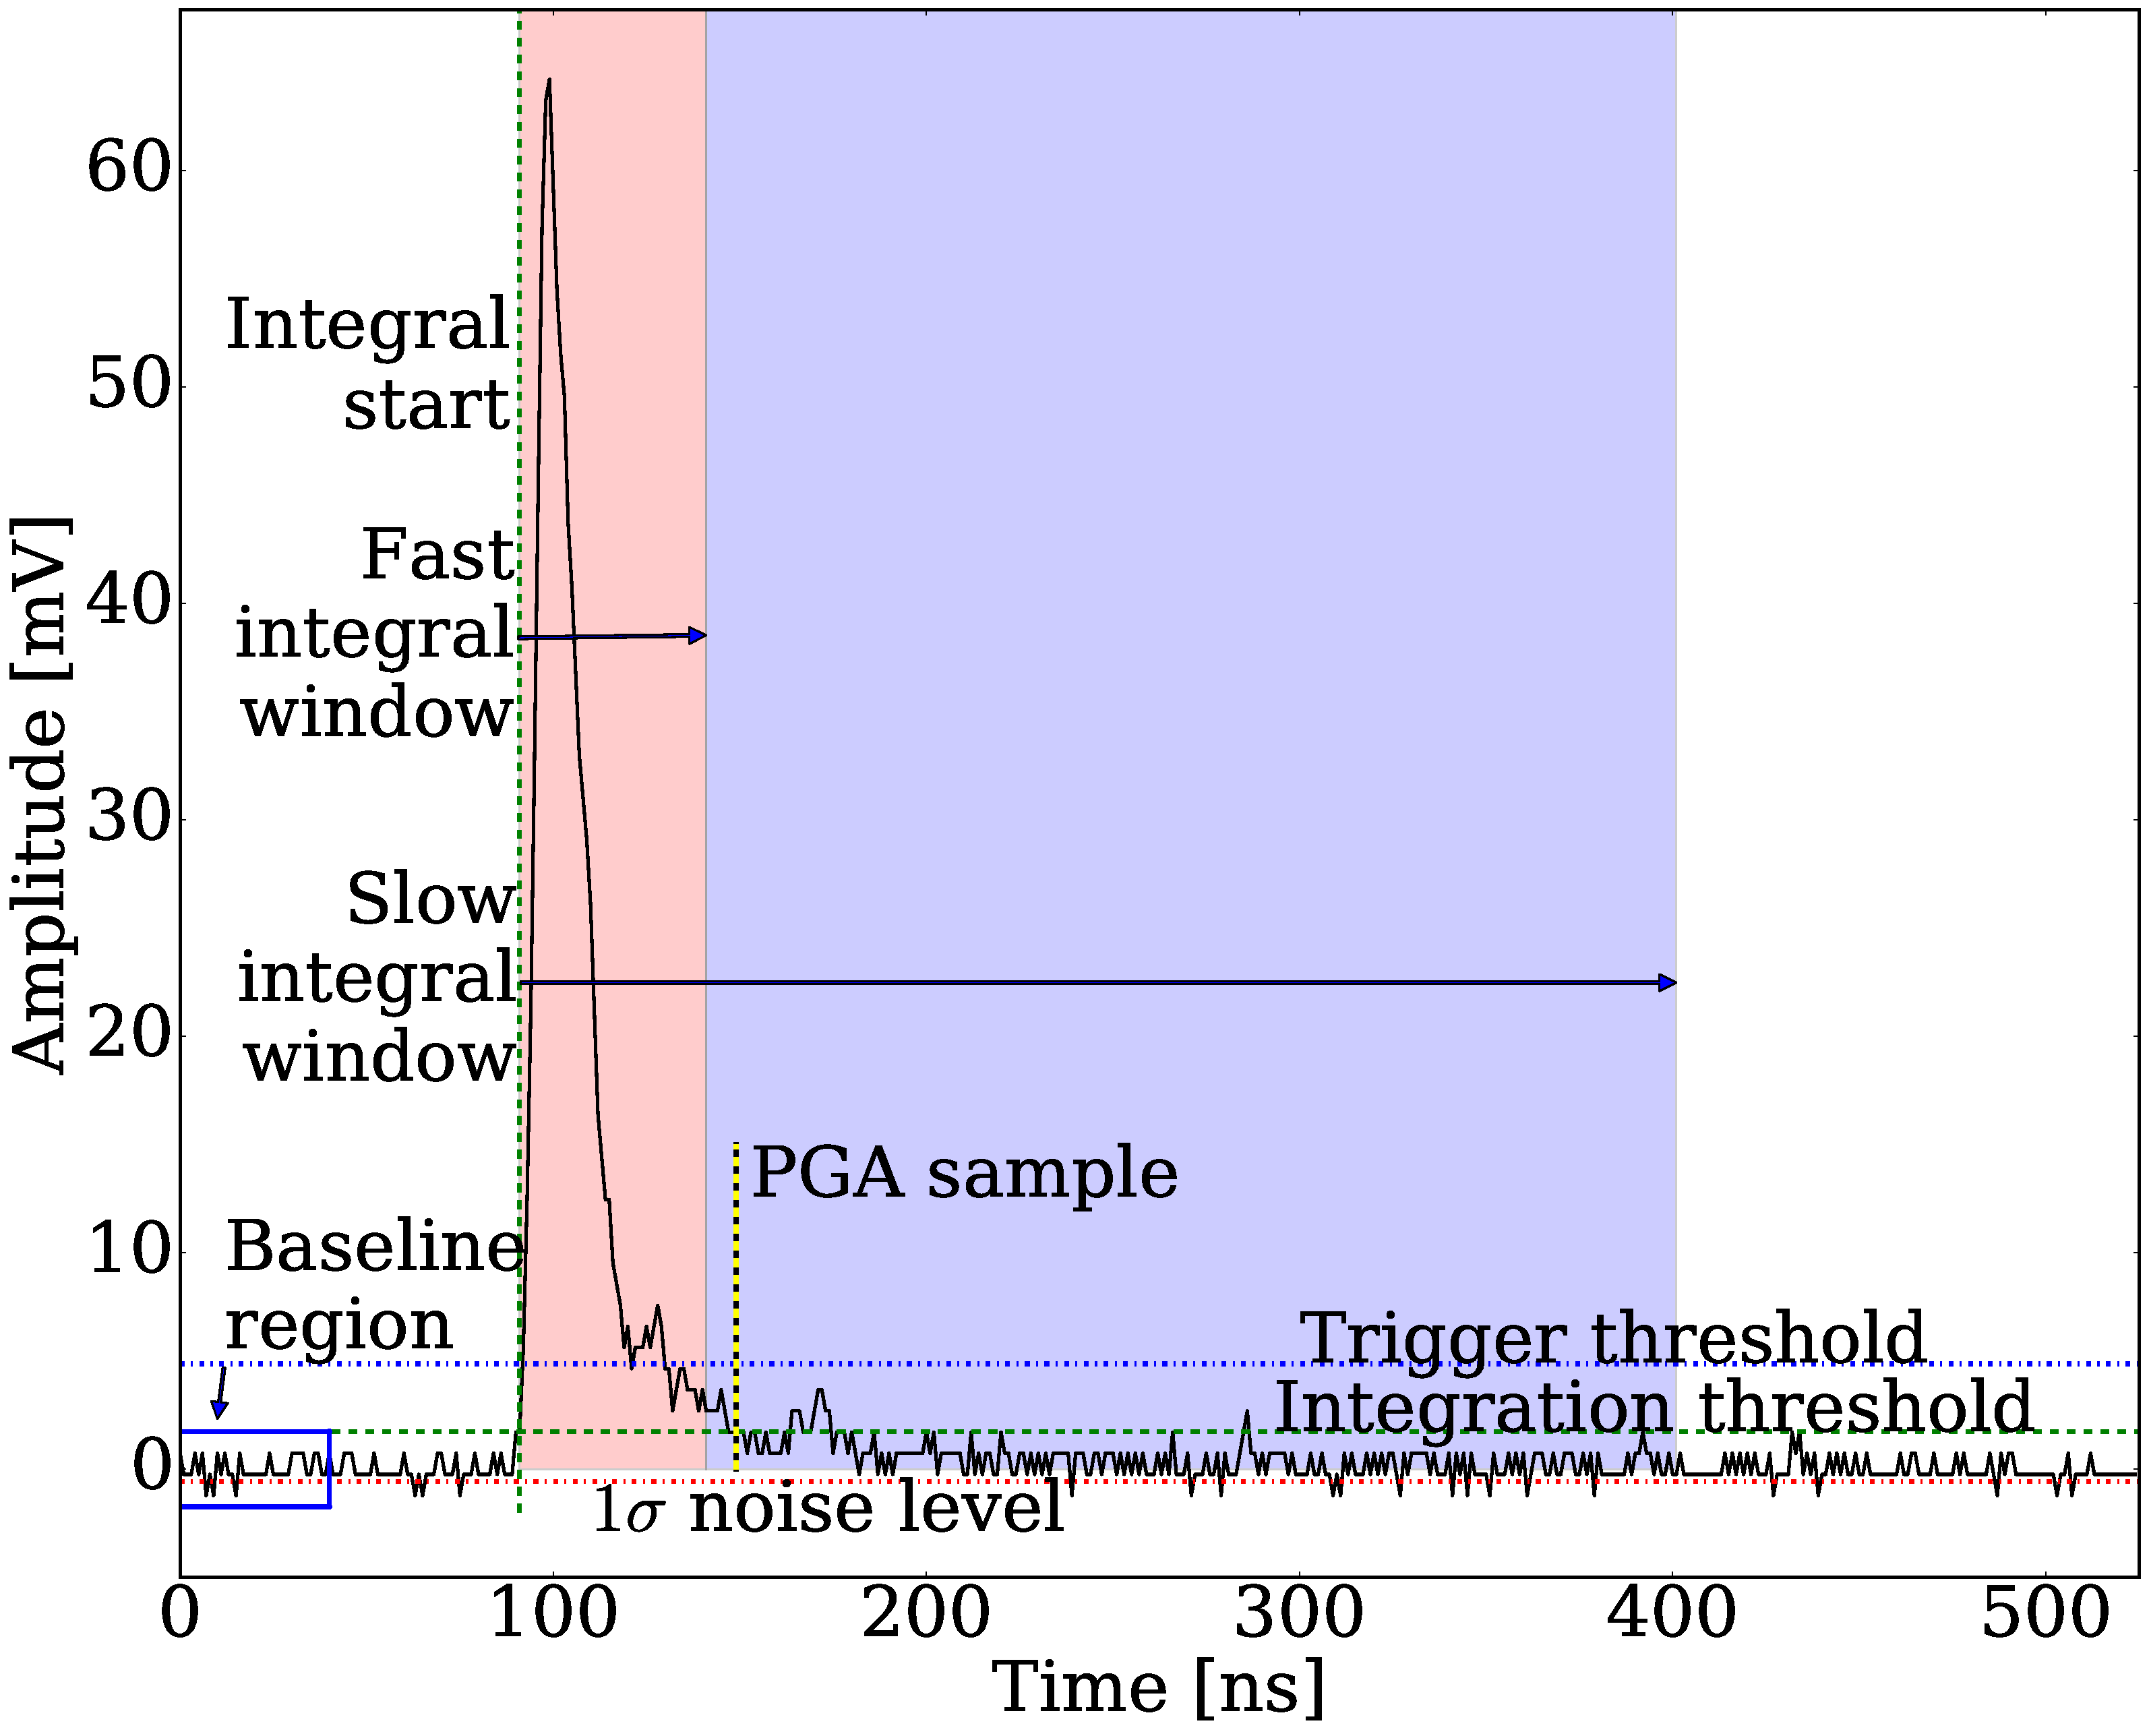
\includegraphics[width=\columnwidth]{figures/psd/fig_annotated_event}
    \caption{A typical gamma event of energy 100 keV. Shown are the trigger and integration thresholds, the ends of the Fast and Slow integral windows, the location of the sample used in the PGA method, the region used for baseline calculations, and the noise level.}\label{fig:psd_waveform}
\end{figure}

\subsection{Charge Comparison Method}

The Charge Comparison Method (CCM)~\cite{Cester:2014,Kaschuck:2005,Liao:2014,WOLSKI:1995,Klein:2002,Ranucci:1998,Soderstrom:2008,Ranucci:1995} predates modern digital computing and was first implemented via passive electronics~\cite{Alexander:1961}. In this method, the baseline-subtracted waveform is integrated over two time windows of different lengths, called \textit{slow} and \textit{fast} or \textit{long} and \textit{short}, respectively. The start of these integral windows is the onset of the pulse, which is defined here as the point at which the waveform exceeds 3$\sigma$ of the baseline RMS (as shown in Figure~\ref{fig:psd_waveform}). The lengths of the two windows are generally set to match the decay modes of the detector. As a NR pulse will decay more slowly than an ER pulse, the slow integral value $I_{\n{slow}}$ will be larger for NR waveforms than for ER, while the fast integral values $I_{\n{fast}}$ are typically comparable for both ER and NR waveforms. We have optimized these times according to the traditional Figure of Merit~\cite{Annand:1987} and found that values of 50~ns for the fast window and 310~ns for the slow window result in optimal discrimination. The discrimination parameter is the ratio of the two integral values,
\begin{equation}
\n{PSD}_{\n{CCM}} = \frac{I_{\n{slow}}}{I_{\n{fast}}}.
\end{equation}

\subsection{Pulse Gradient Analysis}

The Pulse Gradient Analysis method (PGA)~\cite{DMellow:2007} compares the relative height of the peak $H_{\n{peak}}$ to that of a sample $H_{\n{sample}}$ a set time after the peak, here 50~ns. This second sample is averaged with the neighboring 10 samples to reduce noise. As ER pulses decay more quickly than NR pulses, the gradient between the peak and this second sample should be larger for the ER than for the NR. We define the discrimination parameter for this method as the ratio between the two amplitudes,
\begin{equation}
\n{PSD}_{\n{PGA}} = \frac{H_{\n{sample}}}{H_{\n{peak}}}.
\end{equation}

\subsection{Fourier Series Expansion}

Third is a method based on a Fourier series expansion of the waveform ($f(t) = \sum_n A_n \exp (i\omega_n t); A_n = \int_0^T \n{d}t\,f(t) \exp (i\omega_n t)$). Using an approach similar to~\cite{Liu:2010}, the difference between an even order coefficient $A_{2n}$ (odd order $A_{2n+1}$) and the zeroth coefficient $A_0$ (first coefficient $A_1$) is normalized to the zeroth (first) coefficient and then summed:
\begin{equation}
\displaystyle
F_{\n{even}} = \sum_{n} \frac{A_{2n}-A_0}{A_0} \n{~and~} F_{\n{odd}} = \sum_{n} \frac{A_{2n+1}-A_1}{A_1}.
\end{equation}
The expansion is computed to the $30^{th}$ order. The discrimination parameter is then defined as the ratio between these two parameters:
\begin{equation}
\n{PSD}_{\n{FSE}} = \frac{F_{\n{odd}}}{F_{\n{even}}}.
\end{equation}


\subsection{Laplace Transformation}

We also evaluate a discrimination algorithm based on the Laplace transform $\mathcal{L}\{f\} = \int_0^{\infty} \dd t\,f(t)\exp(-st)$. A 9-point moving average is calculated over the trailing edge of the waveform, and the smoothed pulse is then transformed. The transformed waveform is integrated over two frequency ranges, $0.01\1{GHz}\leq s<0.1\1{GHz}$ and $0.1\1{GHz}\leq s<1\1{GHz}$, denoted `low' and `high', respectively, yielding $L_{\n{low}}$ and $L_{\n{high}}$. The frequency ranges are chosen such that the contributions from the $32\1{ns}$ and $270\1{ns}$ decay modes are maximized in each respective range. The discrimination parameter for this method is defined as $L_{\n{high}}-L_{\n{low}}$. However, since this parameter varies significantly with energy, we choose to re-scale it according to
\begin{equation}
\n{PSD}_{\n{LAP}} = I- A \log(B + L_{\n{high}} - L_{\n{low}})
\end{equation}
in order to aide visualization, with the integral of the pulse given as $I$. Parameters $A$ and $B$ are constants chosen as 1/30 and 2, respectively, simply to linearise the plot.

\subsection{Standard Event Fit (SEF)}

\begin{figure}[htbp]
\centering
    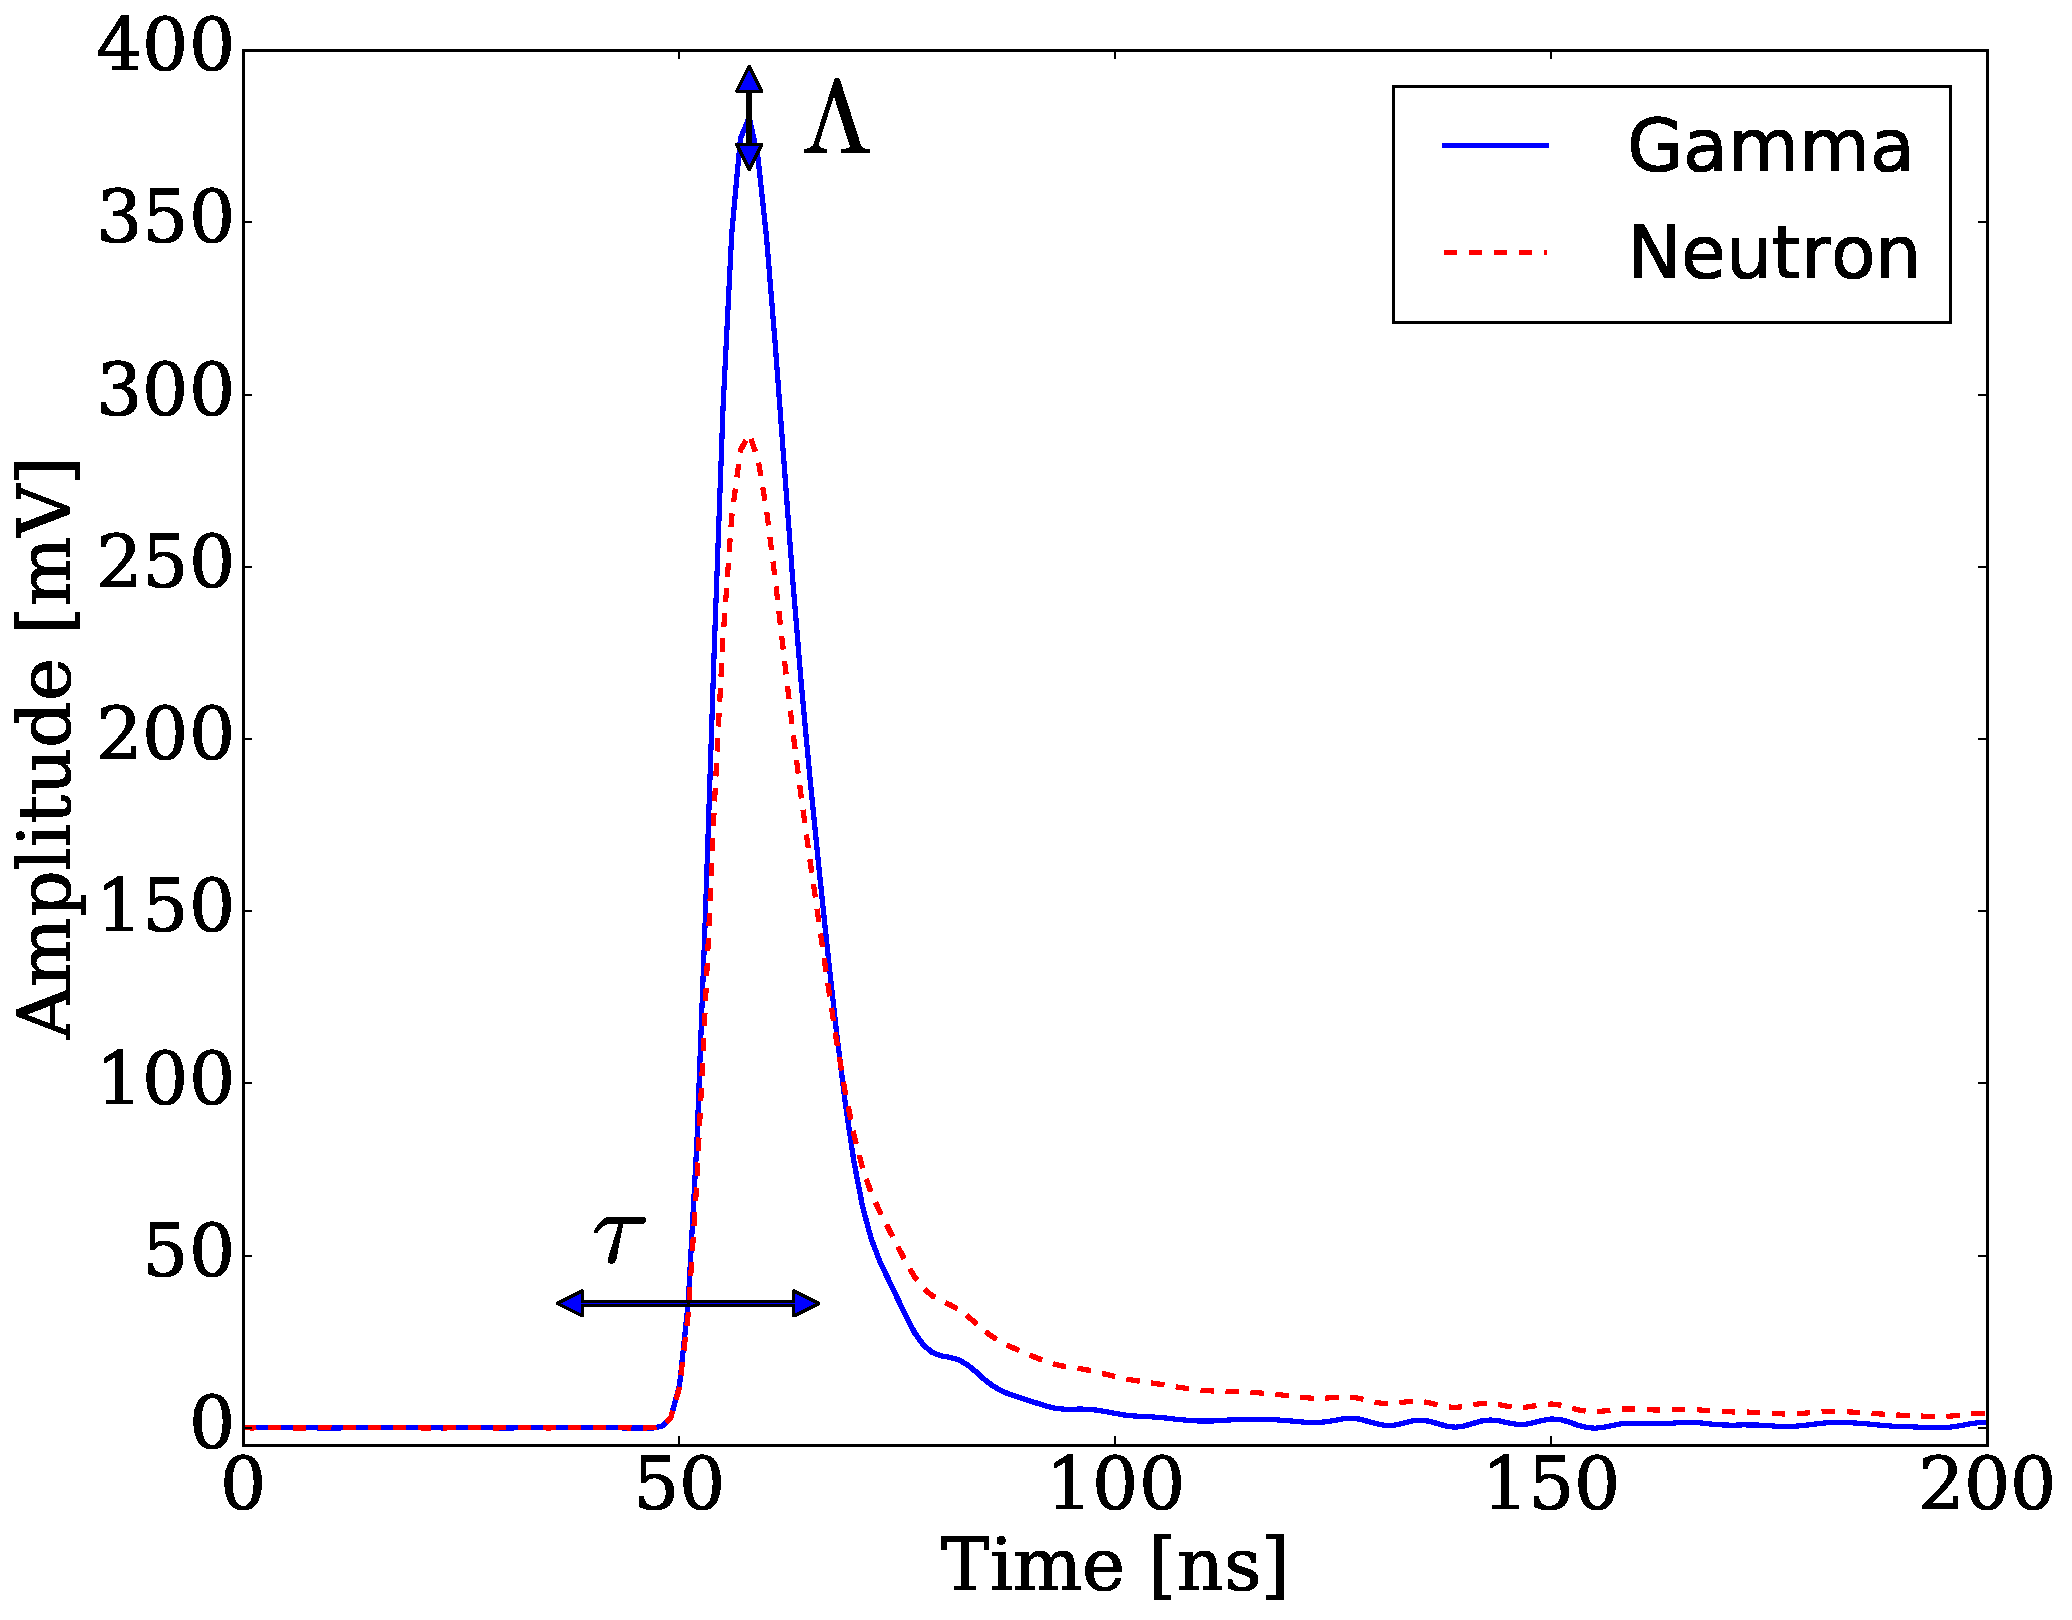
\includegraphics[width=\columnwidth]{figures/psd/fig_standardevents}
    \caption{Standard nuclear recoil (red dotted line) and electronic recoil (blue solid line) events after baseline subtraction. The free fit parameters are a horizontal shift $\tau$ and a vertical scale factor $\Lambda$}\label{fig:stdevents}
\end{figure}

Prior to analysis, $10^5$ events identified as NR or ER by CCM are selected in a narrow energy region around the Compton edge of the 662~keV gamma from $^{137}$Cs. Averaging these waveforms together forms the standard NR or ER event. Both these standard events are then fitted to a given waveform~\cite{Guerrero:2008,Ambers:2011}. While the baseline is fixed to the average of the first 40~ns of the waveform, the free parameters of the fit are a horizontal shift $\tau_{N,E}$ and a scaling factor $\Lambda_{N,E}$, see Figure~\ref{fig:stdevents}. The ER/NR discrimination parameter is then defined as the difference between the chi-squared value $\chi^2_{N,E}$ of each fit, normalized to the vertical scaling fit parameter $\Lambda$:
\begin{equation}
\n{PSD}_{\n{SEF}} = \frac{\chi^2_N}{\Lambda_N} - \frac{\chi^2_E}{\Lambda_E}.
\end{equation}


\section{Analysis}

\begin{figure}[htbp]
\centering
    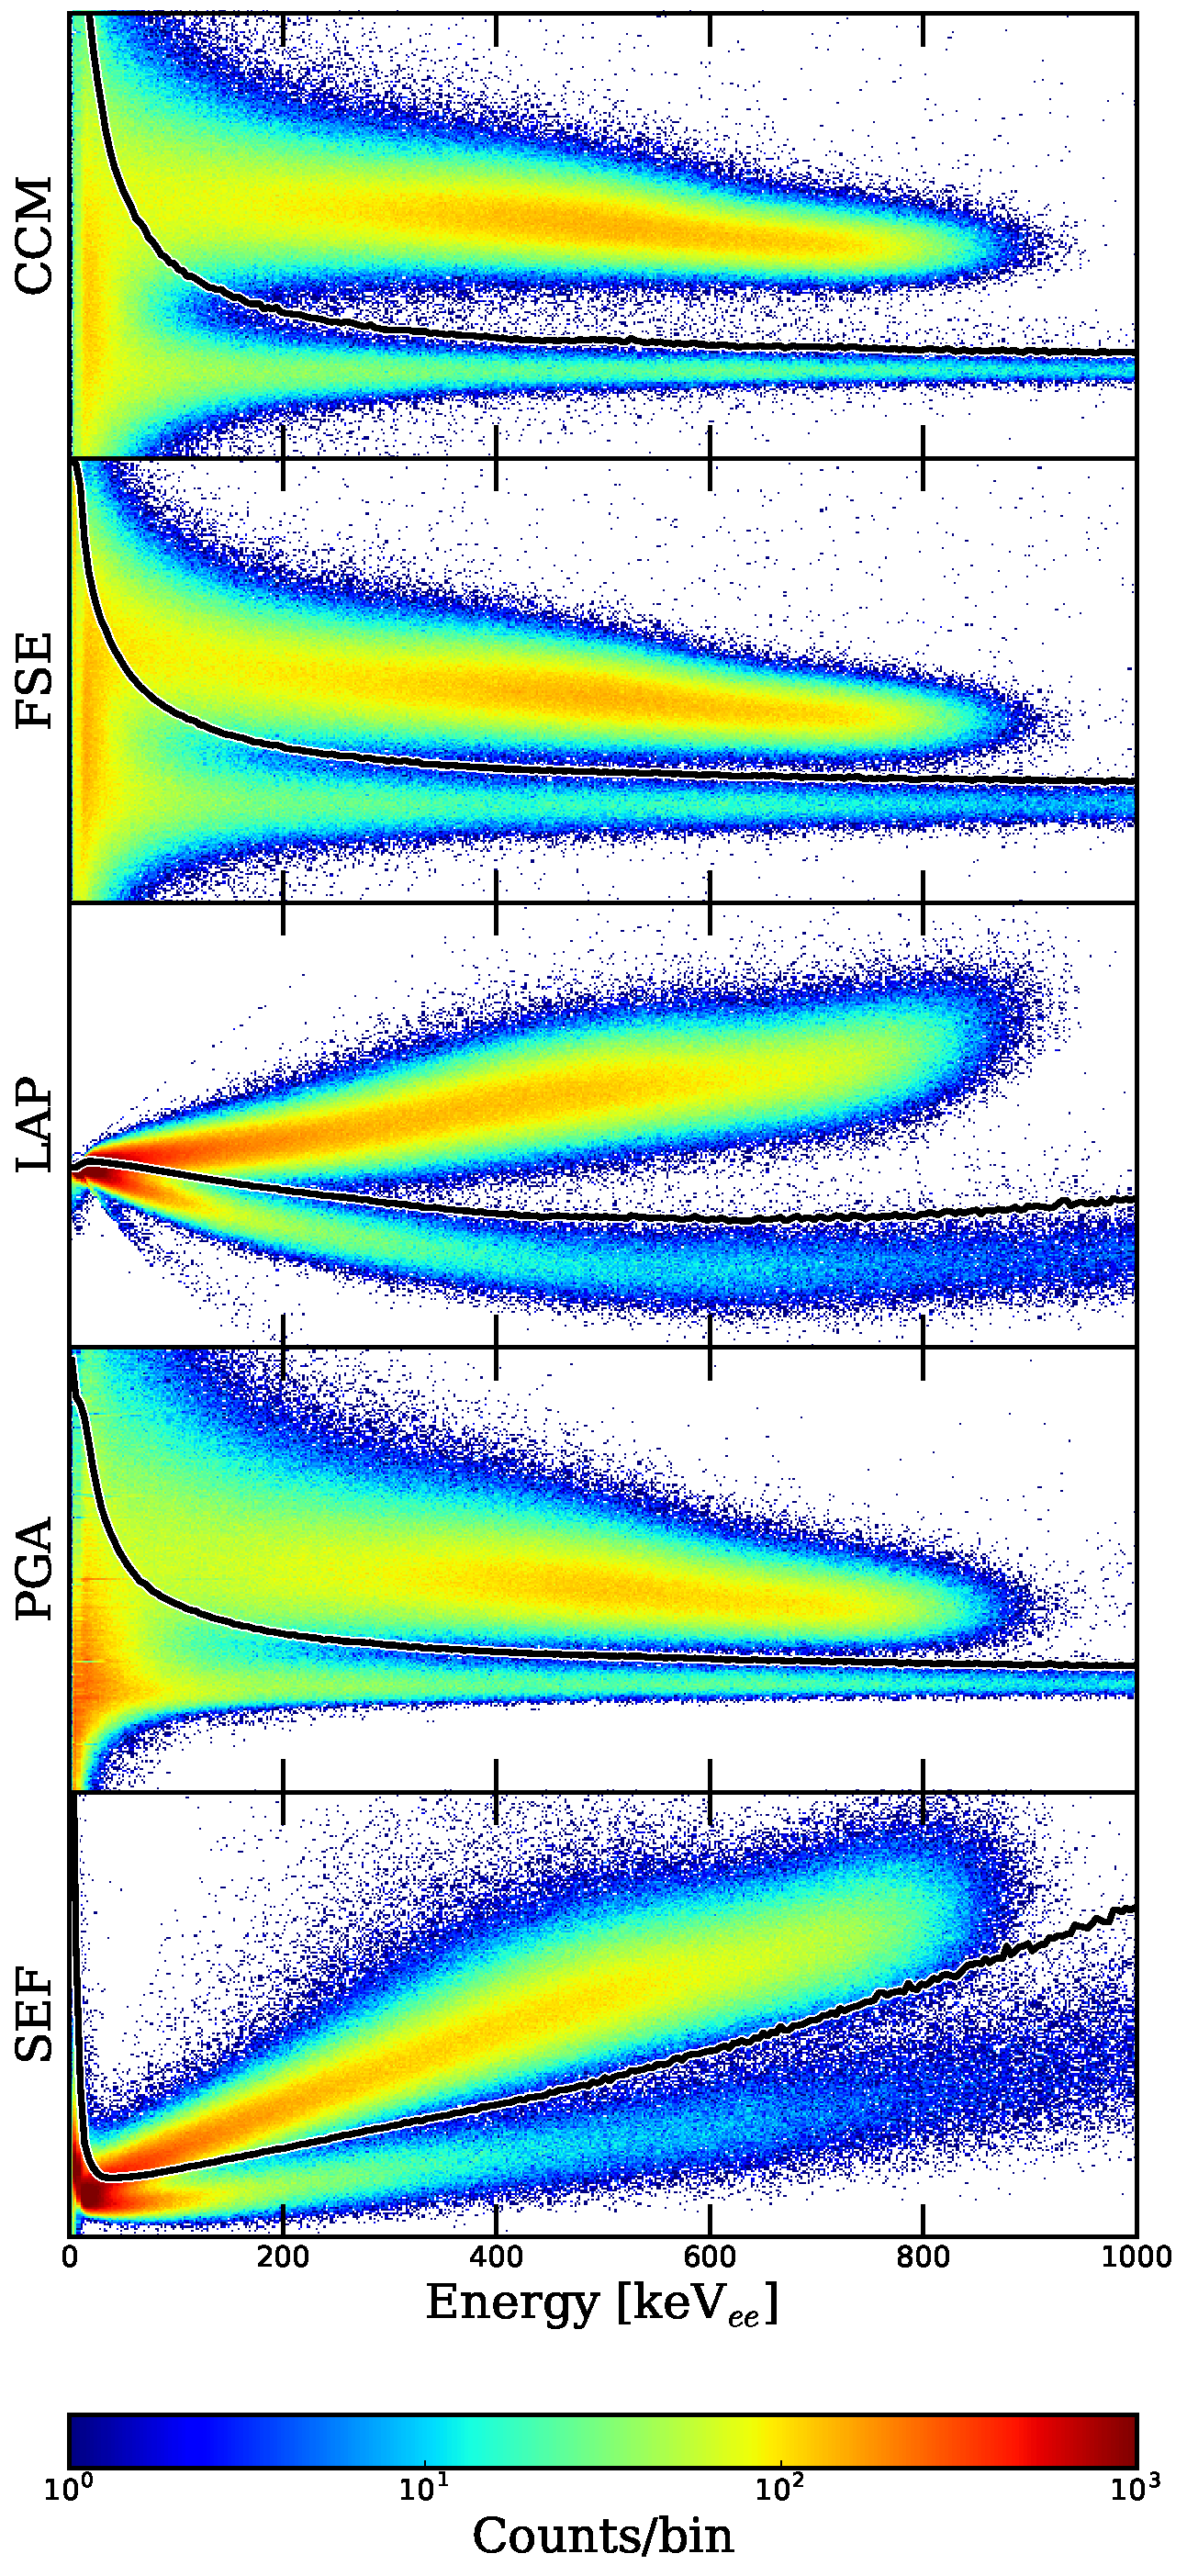
\includegraphics[height=\textheight]{figures/psd/fig_discrim_hists}
    \caption{Plots of various discrimination parameters versus energy for the CCM~(a), FSE~(b), LAP~(c), PGA~(d), and SEF~(e) algorithms. The $99\%$ rejection cut of electronic recoils is also shown in each case. The upper populations are the respective nuclear recoil bands.}\label{fig:discrimination_plot}
\end{figure}

\subsection{Rejection of Electronic Recoils}
The collected data were each processed using the 5~PSD methods discussed in Section~\ref{sec:algorithms}. Rejection cuts for ER events are defined using the datasets taken with various gamma-sources using histograms of the discrimination parameter versus energy. In each energy bin, we consider the one-sided $95\%$, $96\%$, $97\%$, $98\%$ and $99\%$ ER rejection quantiles. Application of the resulting rejection cuts to the overnight background data confirm their performance on neutron datasets.

The event distribution from neutron data are shown in Figure~\ref{fig:discrimination_plot} for all PSD methods together with the one-sided $99\%$ ER rejection cut. For ease of comparison, all PSD parameters were defined such that the NR band is the upper event population.

\subsection{Neutron Flux}

Using the rejection levels defined from the ER band, events are tagged as being either an electronic or nuclear recoil.

Figure~\ref{fig:psd_rateplot} shows the live time-corrected NR energy spectrum, measured from dataset~2, after $99\%$ rejection of ERs using the CCM~algorithm as an example. The expected double-peaked structure due to neutron double scatter events within the detector volume is evident.
The recoil spectrum extends to just below $1\1{MeV_{ee}}$, as expected from $2.5\1{MeV}$ neutrons and the non-linear response spectrum of proton recoil energies in EJ-301 detectors~\cite{Verbinski:1968,Aksoy:1994,Naqvi:1993}. Other algorithms show similar spectra with some variations below $200\1{keV_{ee}}$ which will be discussed in section~\ref{sec:psd_acceptance}.


\begin{figure}[htb]
\centering
    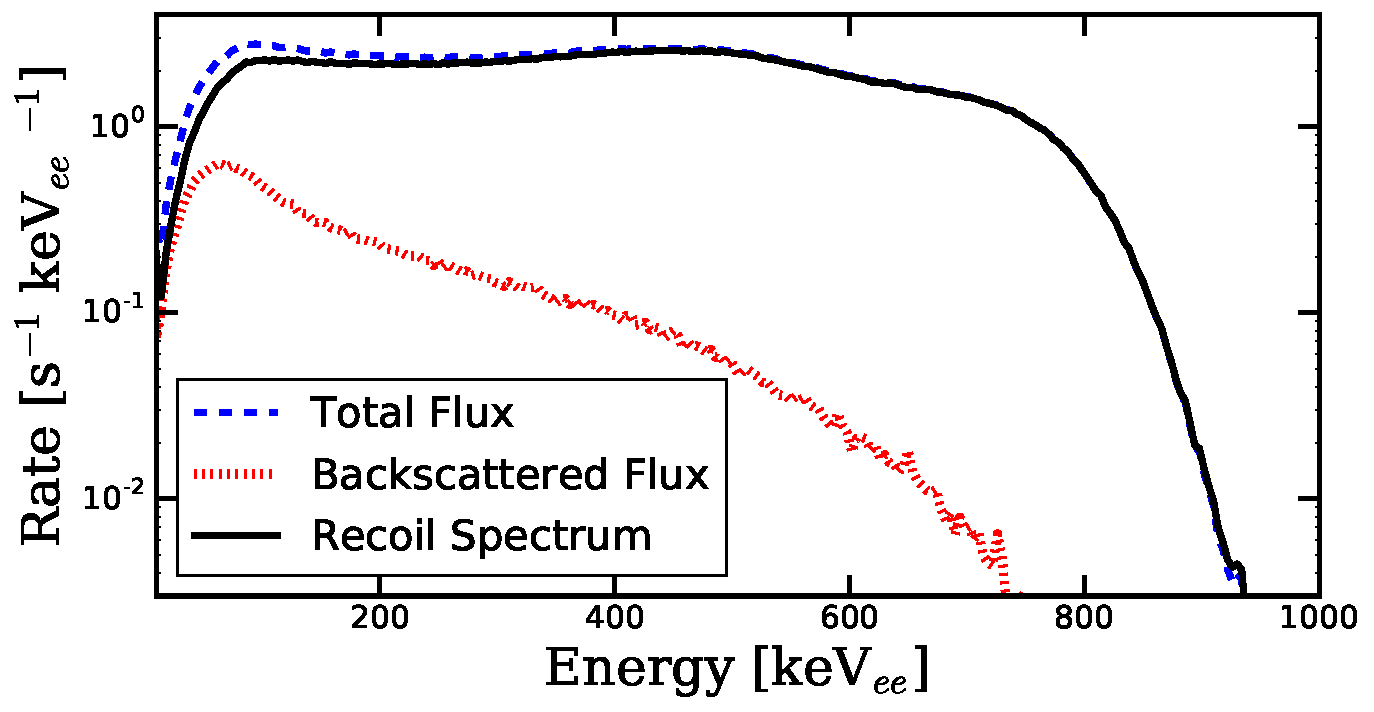
\includegraphics[width=\textwidth]{figures/psd/fig_rate_hists}
    \caption{Nuclear recoil spectra as measured in the EJ-301 detector using the CCM algorithm. The measured backscatter flux (dotted, red) is subtracted from the total measured flux (dashed, blue) in order to obtain the recoil spectrum of $2.5\1{MeV}$ neutrons (solid, black).}\label{fig:psd_rateplot}
\end{figure}

Data collected under the same conditions as dataset~2, but with the shadow cone between the detector and the target is also shown. The observed spectrum is consistent with a range of energies from neutrons scattered off of the air in the experimental hall. The absence of a similar NR spectrum in background data (with no ions on the target), also shown, confirms that these events are related to the beam.

Since we are interested in the efficiency of the EJ-301 detector with regards to detecting $2.5\1{MeV}$ neutrons, we subtract the neutron backscatter rate (Figure \ref{fig:psd_rateplot}, dotted (red) line) from the total neutron rate (Figure \ref{fig:psd_rateplot}, dashed (blue) line). This results in the direct neutron flux at the position of the detector (Figure~\ref{fig:psd_rateplot}, solid (black) line).

\section{Results}\label{sec:psd_acceptance}

\subsection{Acceptance}

Rather than reducing the performance of different PSD algorithms to a single Figure of Merit value (Eq.~\eqref{eq:FOM}), we investigate their energy-dependent behaviour. Specifically, for a given ER discrimination cut, we compare the efficiency of various algorithms using the number of accepted neutrons as a function of energy.

In order to quantify the acceptance of neutrons, a pure band of NRs directly from the beam is required. However, given the reduced performance of all algorithms at low energies, the subsequent overlapping of the NR and ER band, as well as the background from scattered neutrons, no such pure sample is available. We thus invoke a simple statistical algorithm as follows. We use the data taken with the neutron beam incident on the detector to produce the event distributions in the space of PSD parameter $PSD_i$ versus energy $E$, as shown in Figure~\ref{fig:discrimination_plot}. These distributions are corrected for the livetime of each dataset and the integrated beam current, to obtain the time-normalized event density $\varrho_{\n{sig+bck}}(PSD_i,E)$. Similarly, datasets in which the shadow cone was present result in a time-normalized background density of both ER and NR events $\varrho_{\n{bck}}(PSD_i,E)$. Subtracting these two event densities results in an event density $\varrho_{\n{sig}}(PSD_i,E)=\varrho_{\n{sig+bck}}(PSD_i,E)-\varrho_{\n{bck}}(PSD_i,E)$ that is assumed to be representative of the pure band of NRs directly from the beam. This 2D-histogram of event density is then projected onto the energy axis to obtain a "pure" spectrum of all $2.5\1{MeV}$ neutrons detected by the EJ-301 cell for each algorithm.

The acceptance of neutrons is determined by dividing the measured NR spectrum for a given dataset and algorithm (as shown in Figure~\ref{fig:psd_rateplot}) by this "pure" NR spectrum. The resulting energy-dependent acceptance of neutrons at a constant rejection level of ERs is shown in Figure~\ref{fig:psd_acceptance}.

\begin{figure}[htb]
\centering
    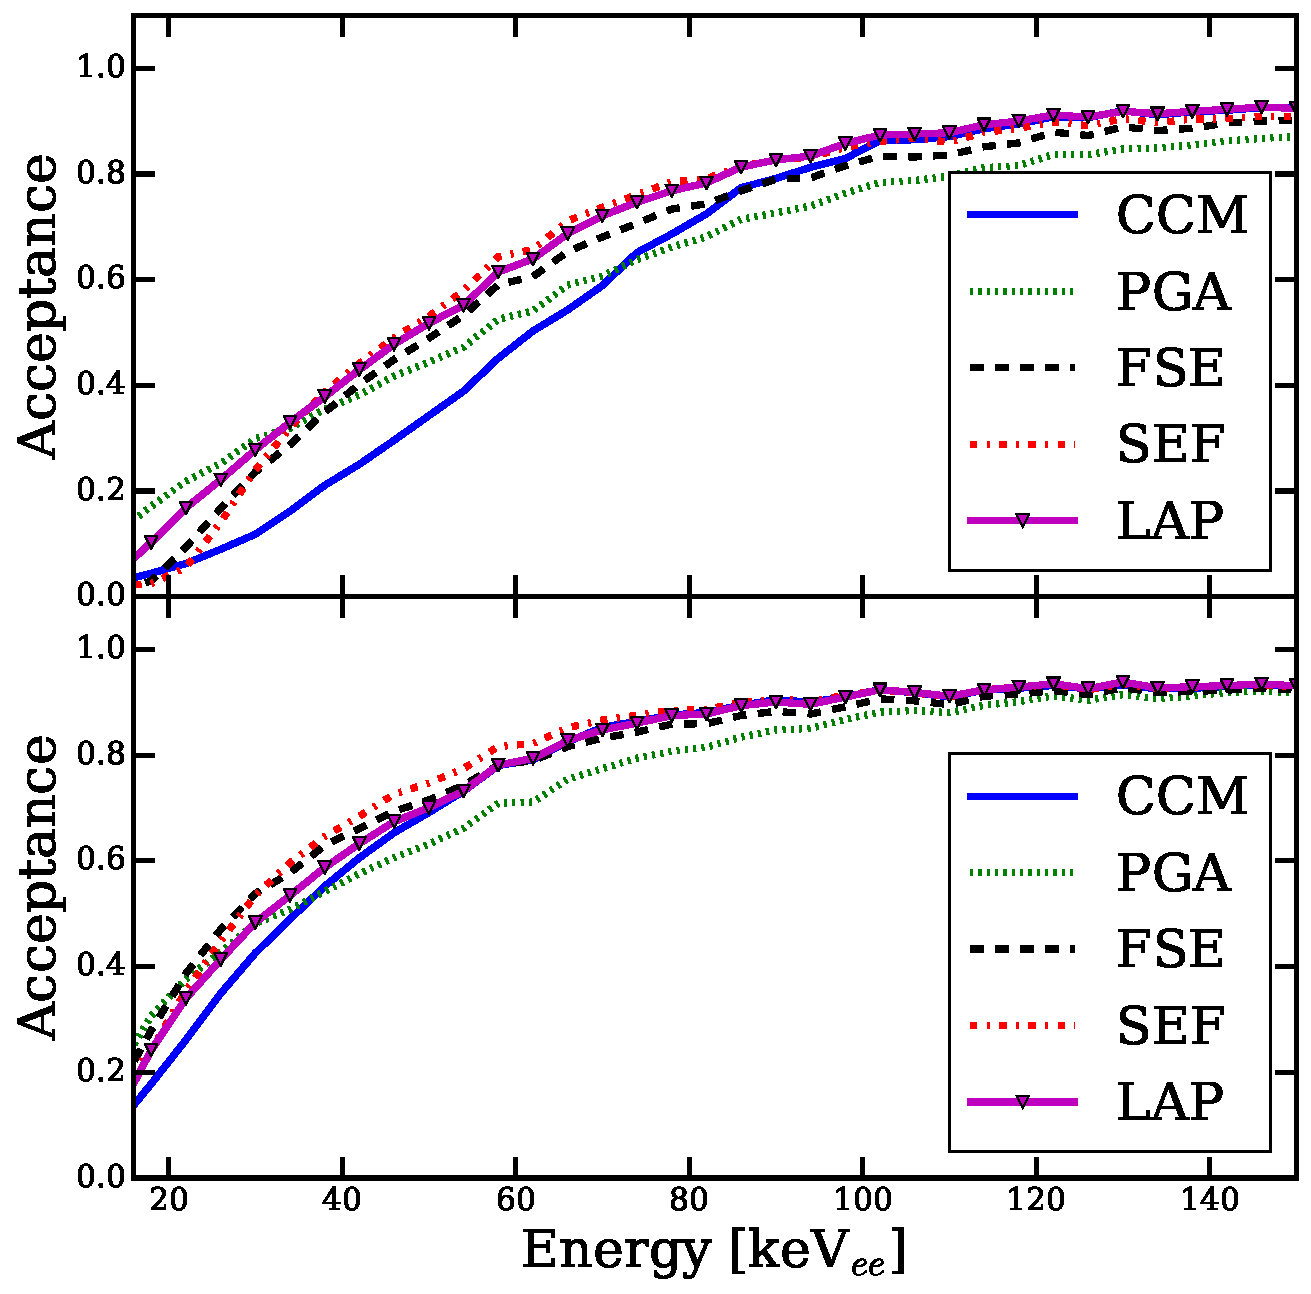
\includegraphics[width = \textwidth]{figures/psd/fig_acceptance}
    \caption{Energy dependence of the fraction of nuclear recoil events that are accepted by each algorithm after $99\%$ (top) and $95\%$ (bottom) rejection of electronic recoils.}\label{fig:psd_acceptance}
\end{figure}

In the low-energy region shown in Figure~\ref{fig:psd_acceptance}, the acceptance of the SEF~algorithm performs best above $30\1{keV_{ee}}$ at $95\%$ rejection of ERs. The acceptances of the LAP and FSE algorithms match each other at this rejection level. As the rejection level of ERs is increased to $99\%$, the acceptance of the LAP algorithm at higher energies is marginally but consistently higher than that of the SEF algorithm. Of note here is that the performance of the traditional CCM algorithm decreases as the rejection criteria for ER events becomes more stringent. Specifically, at $95\%$ rejection of ERs, its acceptance is consistent with that of the SEF, FSE and LAP algorithms, and better than the PGA algorithm. However, at $99\%$ rejection of ERs, the CCM algorithm has the lowest acceptance below $80\1{keV_{ee}}$.

\subsection{Purity of the Nuclear Recoil Spectrum}

At low energy ($<100\1{keV_{ee}}$), there is considerable overlap between the NR and ER bands. Therefore, we not only want to consider the ability of an algorithm to accept neutrons, but also the purity of the resulting NR spectrum. To this end, we construct a reference sample for each algorithm $i$ that contains events that are NRs with high confidence, using those events that are identified by all other algorithms $j\neq i$ as a NR. As a function of energy, we then calculate how many of the events in the reference sample were also tagged as a NR by the algorithm under investigation. The likelihood that an algorithm has tagged an event in the reference sample as a NR is shown in Figure~\ref{fig:n-1_comparison}.

\begin{figure}[htb]
\centering
    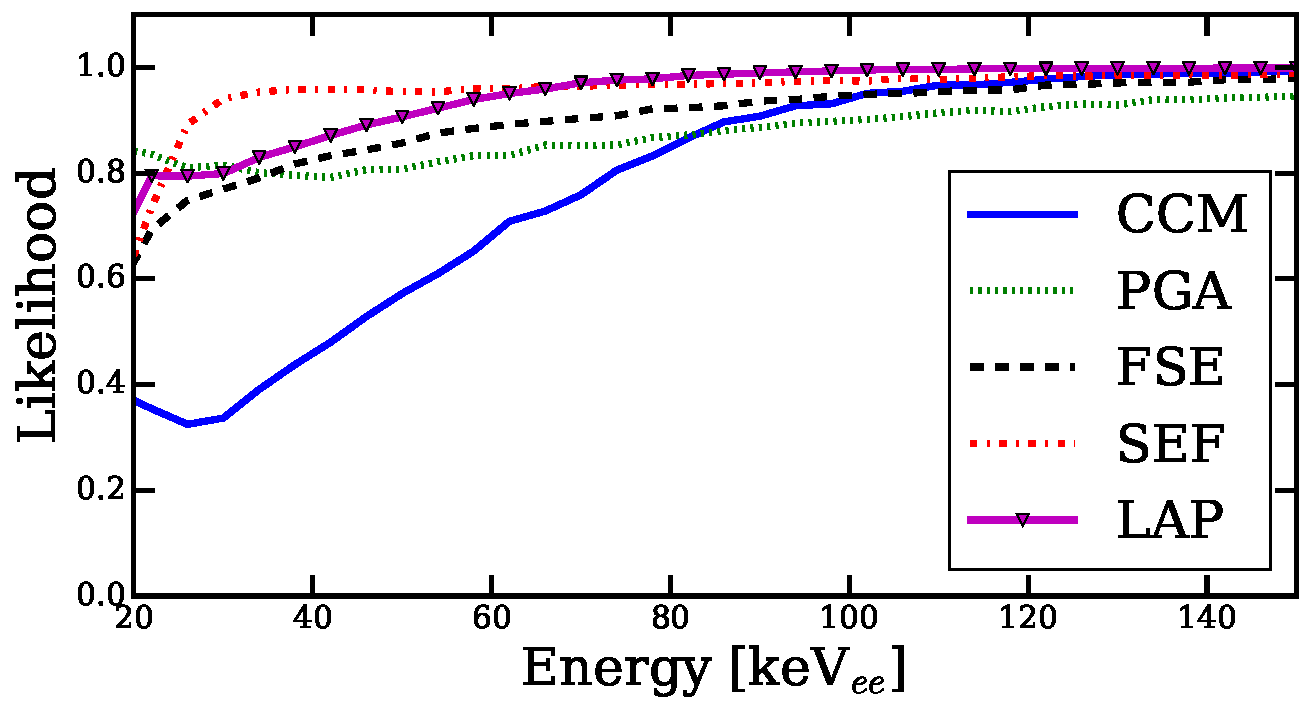
\includegraphics[width = \textwidth]{figures/psd/fig_likelihood}
    \caption{Likelihood that a given algorithm tags an event from a reference sample as being due to a NR. The reference sample consists of events identified as NRs by all algorithms except the algorithm under consideration.}\label{fig:n-1_comparison}
\end{figure}

The inability of the traditional CCM algorithm to identify NR events in a reference sample below $100\1{keV_{ee}}$ is striking. In contrast, the SEF algorithm performs best at low energies and correctly identifies NR events with a likelihood above $95\%$ down to energies below $50\1{keV_{ee}}$. For the SEF algorithm, this likelihood is flat down to energies well below the point at which the acceptance of neutrons for all algorithms has fallen below $50\%$ (compare Figure~\ref{fig:psd_acceptance}). Intriguingly, while the LAP algorithm does provide lower efficiency at low energies, it provides a slightly higher level of confidence that an event is truly a neutron above $\sim75\1{keV_{ee}}$. In contrast to~\cite{DMellow:2007}, we find that the performance of the PGA algorithm is inferior to those of all other algorithms above $80\1{keV_{ee}}$. This observation can be attributed to the fact that the PGA algorithm is based on only two samples of the recorded waveform, thus being highly susceptible to electronic noise.

\subsection{Detector Efficiency}

Table~\ref{tab:psd_datasets} lists the total expected neutron flux of $2.5\1{MeV}$ neutrons through the detector for each dataset. Based on the determined absolute neutron rates from the PTB measurements, we reconstruct the detection efficiency of the detectors as function of energy threshold. The results at $99\%$ rejection of ERs are shown in Figure~\ref{fig:psd_efficiencies}. In addition, the expected efficiency from a MC simulation using the NEFF7 code~\cite{Dietze:1982} is shown in Figure~\ref{fig:psd_efficiencies} for the arrangement in which the detector orientation was $90\degree$ at selected energy thresholds. We find that the efficiency measured in the detector is inconsistent with both the overall efficiency described by the NEFF7 code, as well as the functional dependence of the efficiency on the threshold. Independent of the PSD algorithm, the measured efficiency in the EJ-301 detector is lower and less threshold-dependent than that described by the NEFF7 code. We thus conclude that the NEFF7 code can currently not be used to obtain accurate detection efficiency information for EJ-301 liquid scintillator cells.

\begin{figure}[htb]
\centering
    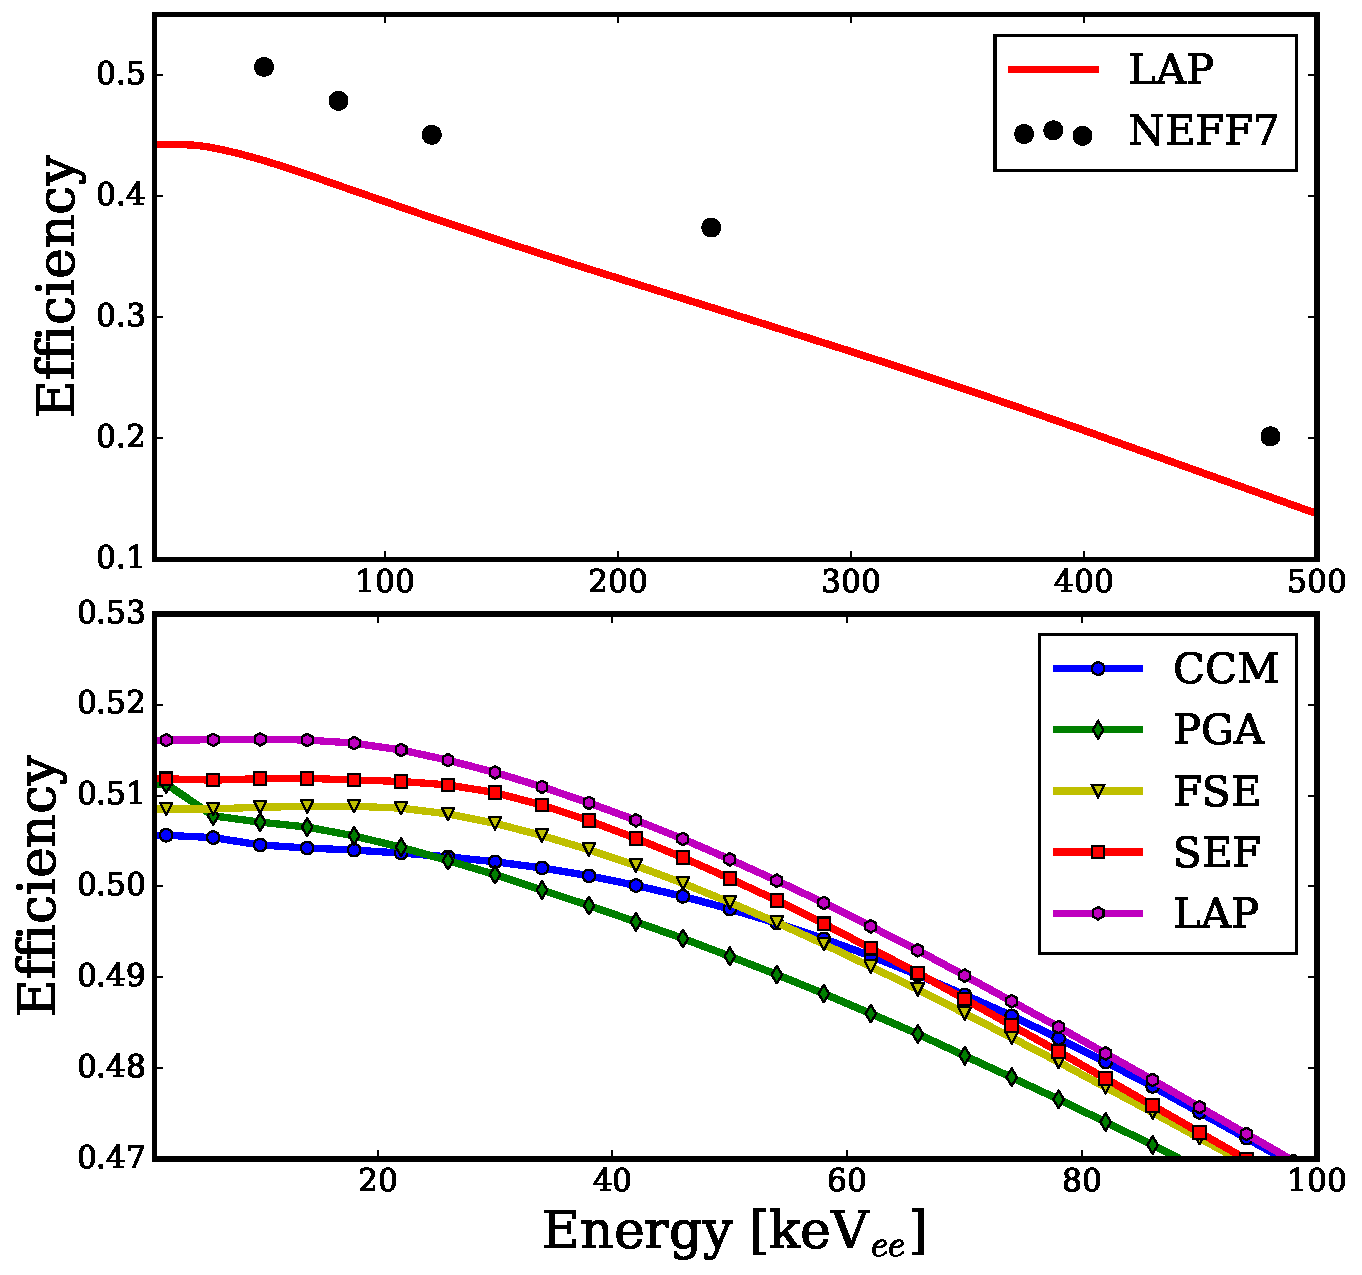
\includegraphics[width = \textwidth]{figures/psd/fig_efficiency}
    \caption{(Top) Comparison between the threshold-dependent efficiency of the SEF algorithm and the prediction from the NEFF7 code in EJ-301. The detector is orientated at $90\degree$. (Bottom) The efficiency of all algorithm as a function of threshold. Note the different energy ranges.}\label{fig:psd_efficiencies}
\end{figure}

The PGA algorithm has the lowest efficiency above $30\1{keV_{ee}}$, consistent with it having a poorer ability to accept neutrons at a given rejection level of ERs. The traditional CCM algorithm has poor efficiency below $60\1{keV_{ee}}$ when compared to the three newer algorithms FSE, SEF and LAP. The LAP algorithm has the highest efficiency at all energy thresholds. This observation can be ascribed to its higher acceptance of NRs at higher energies. The LAP algorithm is better at discriminating between the NR and ER band at higher energies, as the ER band of the SEF algorithm spreads as the energy increases (compare Figure~\ref{fig:discrimination_plot}), while the ER band of the LAP algorithm has a more consistent width.


\subsection{Processing Speed Benchmarks}

The processing speed of each algorithm was measured on a dataset of approximately $500\,000$ events (about $550\1{MB}$), both with and without the C++ compiler optimizations available in the GNU compiler collection version 4.8.3, using a standard desktop computer. The results are show in Table~\ref{tab:benchmarks}. From this we see that the increased low-energy performance of the SEF algorithm comes at a very high computational cost.

\begin{table}[htbp]
\centering
    \caption{Processing rates of the different algorithms, given in units of waveforms/sec, using a standard desktop computer.}\label{tab:benchmarks}
    \begin{tabular}{c p{26mm}p{26mm}}
    Algorithm & Rate without \newline optimizations & Rate with \newline optimizations \\
    \hline
    PGA & $1.6\times10^6$ & $4.8\times10^6$ \\
    CCM & $168\,000$ & $1.6\times10^6$ \\
    FSE & $4\,300$ & $84\,000$ \\
    LAP & $1\,100$ & $16\,000$ \\
    SEF & 110 & 230 \\ \hline
    \end{tabular}
\end{table}

\section{Conclusions}

We have compared the performance of five different pulse shape discrimination algorithms using a commercial liquid scintillator cell. The studied algorithms include the avant-garde algorithms Standard Event Fit SEF, Fourier-Series Expansion FSE, and Laplace Transform LAP in addition to the traditional Charge Comparison Method CCM and Pulse-Gradient Analysis PGA. The energy-dependent behaviour of all five algorithms was discussed as a better means of describing PSD algorithms than the Figure of Merit previously used in the literature.

Specifically, we considered the ability of each algorithm to accept NRs as function of recoil energy, as well as the purity of the resulting NR sample. We find that at $99\%$ rejection of ER background events and above $80\1{keV_{ee}}$, the PGA algorithm accepts the fewest number of NRs and is the least likely to identify a NR event from a reference sample. The CCM algorithm performs better than the PGA method, but a marked deterioration in the performance of the CCM algorithm is observed as the rejection level of ER events becomes more stringent.

Both the SEF algorithm and the LAP algorithm display improved performance compared to the traditional methods considered. The SEF algorithm is more likely to accept NRs from a reference sample at low energies, and it provides a higher acceptance of NR events below $80\1{keV_{ee}}$. The LAP method however provides a slightly higher efficiency overall for the detection of NRs in EJ-301 due to a better-resolved ER band at higher energies.

With this improved performance of discrimination and the understanding of the energy dependence of this performance, we can now proceed to understand the neutron generator.


% neutron generator
% NG paper, v1.0

\chapter{Characterzation of the neutron generator}\label{ch:ng}

\paragraph{Abstract} Now that the performance of the neutron detectors has been measured (see Chapter~\ref{ch:psd}), we proceed to focus on the deuterium-deuterium plasma fusion neutron generator. We measured the isotropy of the emission, the energy spectrum, and the depdencence of the neutron production rate on the operational parameters of the generator. These results were published as Lang et al, Nuclear Instrumentation and Methods, A879:31-38 (2017), and are reproduced here.

\section{Introduction}

Neutron generators are a convenient, commercially available source of neutrons widely used in science and engineering. They can easily achieve a tuneable neutron flux of $10^6\1{n/s}$ with some generators operating above the $10^{10}\1{n/s}$ range, they pose no or only minimal safety concerns when turned off, and they are available in a variety of configurations. The latest advances in the field of compact sealed-tube neutron generators toward the development of smaller, lighter and less expensive systems further extend their applicability.

Two main reactions are exploited in such generators: deuterium-tritium fusion yielding $14.1\1{MeV}$ neutrons, and deuterium-deuterium fusion yielding $2.45\1{MeV}$ neutrons in the center-of-mass frame. Two operating principles are commonly employed to induce fusion. One is to accelerate a beam of deuterium ions onto a solid state target which contains either deuterium or tritium. Another principle is the fusion of ions in a plasma in the presence of a high voltage potential. Indeed, there are detailed discussions of the characteristics of deuterium-tritium generators~\cite{Guillame:1971}, deuterium-deuterium generators~\cite{Miley:1997,Miley:1999,Miley:2000} as well as neutron generators in general~\cite{CRC,Chernikova:2014}. However, to our knowledge, the measurements reported here represent the first complete characterization of a deuterium-deuterium plasma fusion generator, including the determination of absolute neutron yield, neutron energy spectrum and emission anisotropy.

\section{Setup} \label{sec:ng_setup}

\subsection{Neutron Generator}

The neutron generator characterized in this work is a model 35-DD-W-S deuterium-deuterium plasma fusion neutron generator manufactured by NSD/Gradel-Fusion. This generator produces $2.45\1{MeV}$ neutrons based on the fusion of deuterium

\begin{equation}
\rm{{}^2D + {}^2D } \rightarrow \rm{{}^3He~}(0.82\1{MeV}) + \rm{n~} (2.45\1{MeV}) {\rm .} \label{eqn:main_reaction}
\end{equation}

The generator is capable of delivering neutron fluxes up to $10^7\1{n/s}$. Given our particular application of this generator in the field of direct dark matter detectors~\cite{Aprile:2015uzo}, it was modified to enable stable operation even at fluxes as \textit{low} as $10\1{n/s}$. The neutron generator has a cylindrical shape with a length of $940\1{mm}$ and a diameter of $138\1{mm}$. It has a standalone high voltage power supply module, a slow control program to monitor system parameters, and a water cooling loop.

The working principle of the neutron generator is based on inertial electrostatic confinement (IEC). The generator has a fusion chamber filled with deuterium gas. The deuterium pressure is reduced to a level that allows for plasma ignition by glow discharge (Paschen's law). The primary source of neutrons is considered to be the plasma in the volume surrounded by the cathode. Deuterium gas in the fusion chamber is ionized and the resulting ions are accelerated toward the cathode field cage. Once inside the field cage, the ionized gas is confined by applying a high voltage ranging between $10-100\1{kV}$. When the necessary conditions to overcome the Coulomb barrier are met, fusion occurs, emitting approximately mono-energetic $2.45\1{MeV}$ neutrons.

\subsection{Liquid Scintillators}

We use two liquid scintillator detectors, a 3"$ \times$3" EJ301 cell and a 2"$\times$2" NE213 cell, to measure the neutron energy spectrum and relative flux. The scintillator used in these detectors is identical, apart from the manufacturer~\cite{ej_datasheet}. Liquid scintillators are very popular for fast neutron detection as they can easily be shaped into the desired size and geometry of a given application. The process of elastic scattering by neutrons off the protons found in the hydrocarbon molecules produces prompt scintillation that offers excellent timing performance. Such nuclear recoils exhibit greater ionization density rates than electronic recoils that are induced by various backgrounds. Consequently, the ionization tracks of nuclear recoils produce higher yields of delayed fluorescence, resulting in scintillation pulses that decay more slowly than those of electronic recoils of comparable energy. The different pulse shapes that arise from electronic and nuclear recoils in liquid scintillators can thus be exploited using pulse shape discrimination methods~\cite{Brooks:1959,Kuchnir:1968,Perkins:1979,Lang:2016xks}. Additionally, if the detector response to neutrons of specific energies is well known, these detectors can be used to reconstruct the energy spectrum of the incident neutron flux~\cite{Klein:2002,Verbinski:1968}.

The EJ301 detector cell was optically coupled to a ETEL 9821KB photomultiplier (PMT) which was operated at a voltage of $1700\1{V}$. The anode signal of the PMT was acquired using a CAEN DT5751 digitizer, which samples at 1 GHz with 10 bit resolution and has a 1 V dynamic range. The NE213 detector cell was coupled to an XP2020 PMT via a short lucite light guide. The PMT was operated at a voltage of $-1950\1{V}$. Standard nuclear electronics modules were used for analogue signal processing. A signal proportional to the total amount of scintillation light produced in the detector cell (pulse height) was derived from the ninth PMT dynode. A second signal related to the decay time of the light pulse (pulse shape) was derived from the PMT anode using the zero-crossing technique. The two signals were digitized using pulse-height sensitive ADCs and a PC based multi-parameter data acquisition system. Deuterium-deuterium IEC fusion devices are known to produce bremsstrahlung in addition to neutrons~\cite{Luo:2010}. Therefore we operated the liquid scintillator detectors with lead shielding.

The gain of the PMT in the NE213 detector was constantly measured and adjusted using a feedback loop. This was constructed with an integrated LED, that gave constant light pulses at a rate of $65\1{Hz}$, and a voltage added to the bias voltage based on the PMT's response to the LED pulse. This setup allowed for a constant gain during the long measurements required for determining the energy spectrum (section~\ref{sec:en_spectrum}).

\subsection{De Pangher Long Counter}
We use a De Pangher Long Counter to measure the absolute neutron flux. This detector is made of concentric layers of polyethylene and borated polyethylene. The borated polyethylene shields the detector from neutrons entering the detector through its side wall, whereas incident neutrons from the source, which enter through the planar surface, are thermalized by the polyethylene. At the center of the Long Counter is a tube filled with BF$_3$ that is enriched in $^{11}$B. Thermalized neutrons that are scattered into this volume can be captured, producing an alpha through the $\mathrm{^{11}B(n, \alpha)^{7}Li}$ reaction. The detection of the emitted alpha particle produces a unique signal in the detector that is used to tag neutrons.

The Long Counter has the ability to measure neutron fluxes with a response that is almost independent of neutron energy in the range from a few keV to almost $10\1{MeV}$. Their high sensitivity allows them to be used to measure low neutron fluxes. Additionally, they are directional, which is necessary to control the impact of in-scattered neutrons~\cite{Nolte:2011}.

\subsection{Experimental Setup}

\begin{figure}[!htb]
\centering
    \includegraphics[width = \columnwidth, clip=true, trim =0 0 0 0]{figures/ng/setup_image_straightened_red}
    \caption{The experimental setup at PTB. The neutron generator is located at the center of the circle with the Long Counter at a radial distance of $1569\1{mm}$. On the left hand side, the NE213 detector can be seen at a distance of $2069\1{mm}$ and at polar angle $230\degree$.}\label{fig:ptb_setup}
\end{figure}

\begin{figure}[!htb]
\centering
    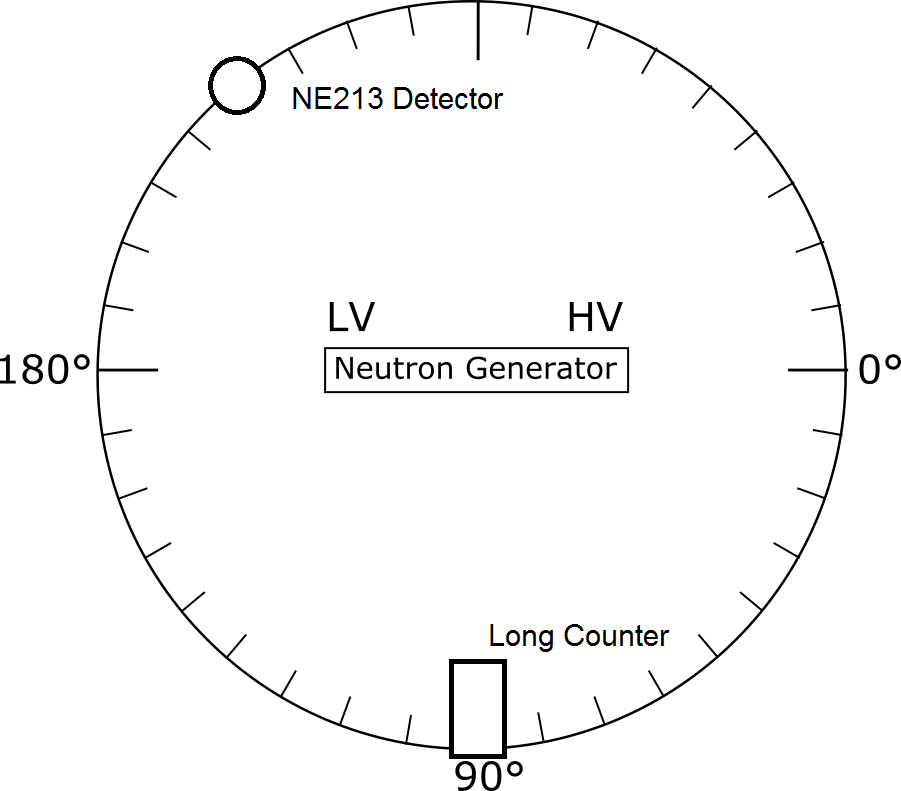
\includegraphics[width = 0.9\columnwidth, clip=true, trim= 0 0 0 0]{figures/ng/coordinate_schematic_v2_0} % left lower right upper
    \caption{The coordinate system used at PTB. The schematic shows the neutron generator from above, with its high voltage  (HV) end taken to be at $0\degree$ polar angle and its low voltage (LV) end taken to be $180\degree$ polar angle. Also shown are the Long Counter at $90\degree$ and the NE213 detector at $230\degree$, as the detectors were placed when Figure~\ref{fig:ptb_setup} was taken.}\label{fig:ptb_coordinates}
\end{figure}

Measurements of the neutron flux were performed both at Purdue University and at the Physikalisch-Technische Bundesanstalt (PTB). Figure~\ref{fig:ptb_setup} shows the experimental setup at PTB. The neutron generator was placed with its horizontal axis at the center of the experimental facility. We define the polar angle such that the direction perpendicular to the axis of the neutron generator is $90\degree$, as shown in Fig.~\ref{fig:ptb_coordinates}. All distances in this section are measured from the center of the neutron generator to the front face of the detector in question.

To measure the neutron energy spectrum, a NE213 detector was placed at a radial distance of $865\1{mm}$ from the generator, facing it at a $90\degree$ polar angle. These measurements were taken for a duration of $6.0\1{hours}$ while the neutron generator was operated at $50\1{kV}$ and $2.5\1{mA}$. To be able to perform background discrimination and subtraction, data were also collected for $21.1\1{hours}$ while the neutron generator was off.

Additionally, data were taken with a shadow cone placed between the neutron generator and the Long Counter, where the Long Counter was placed at two different radii. These measurements were used to verify that the Monte Carlo simulations of the experimental setup correctly accounts for the number of neutrons scattered off the air into the Long Counter.

For the measurements of the angular emission (section~\ref{sec:angular}), the Long Counter was placed on a radial arm at a distance of $1569\1{mm}$ from the neutron generator but at various polar angles. A 3''$\times$3'' EJ301 detector was placed at a distance of $2000\1{mm}$ at a fixed angle of $230\degree$ in order to have a permanent measurement of the stability of the generator during the angular scan.

The functional dependence of the neutron flux on the applied voltage and current were determined using three EJ301 liquid scintillator cells at Purdue in various orientations. The response of these detectors to~$2.45\1{MeV}$ neutrons has previously been characterized~\cite{Lang:2016xks}. Furthermore, the functional dependence and absolute flux were measured at PTB with the Long Counter at a radial distance of $1569\1{mm}$ and a polar angle of $90\degree$.


\section{Monte Carlo Simulation}

We have developed a detailed Monte Carlo simulation of the experimental setup in order to assist with the interpretation of the obtained data. The simulation was developed using the GEANT4 toolkit~\cite{Geant4}.  Technical drawings of the neutron generator and its interior, as well as the three different neutron detectors, were used to create a complete description of the major components that can produce significant scattering of neutrons.

\subsection{Physics List in GEANT4}

This simulation made use of version \texttt{9.4-patch02} of the GEANT4 toolkit. Since the energy of the neutrons of interest is below $20\1{MeV}$, we use the \texttt{High Precision} physics list, with \texttt{G4NDL 3.14}. This list contains cross-sections down to thermal energies in order to accurately describe the elastic, inelastic and capture processes of neutrons in the Long Counter. The radioactive $\alpha$, $\beta^{+}$, $\beta^{-}$ or electron capture decays are simulated using \texttt{G4RadioactiveDecay}. Information about the half-lives, nuclear level structure, decay branching ratios, and the energies of decay processes are taken from the Evaluated Nuclear Structure Data Files (ENSDF)~\cite{Bhat:1992}.

The tracking of particles in GEANT4 is divided into spatial steps. The length of these steps is automatically set depending on the energy and type of each particle, as well as the material it is propagating through. For each interaction, we record the position, deposited energy, particle type, initial energy of the particle, and the process responsible for the energy loss.

\subsection{Neutron Generator Model}\label{sec:initialneutronspectrum}

The description of the neutron generator in the GEANT4 toolkit is reproduced from technical drawings and information provided by the manufacturer, NSD/Gradel Fusion. The important internal components included in the simulation are the reaction chamber and cathode, high voltage feedthrough, getter pump, and the water cooling system. The deuterium gas conditions inside the fusion chamber were modelled using the known pressure of the deuterium gas. We assumed homogeneous neutron production within the cathode volume, producing an isotropic neutron flux. This assumption is consistent with the measured angular neutron flux (section~\ref{sec:angular}) and the energy spectrum measured at two different polar angles (section~\ref{sec:en_spectrum}).

The energy spectrum used as an input in the GEANT4 simulation was calculated using the known energy-dependent differential cross-section of deuterium-deuterium fusion. The characteristic deuteron energy was described by a Gaussian distribution with a mean of~$30\1{keV}$ and sigma of~$3\1{keV}$. While this is consistent with the applied high voltages of $40\1{kV}$ and $50\1{kV}$, at which measurements of the energy spectrum were obtained, assumed average kinetic energies between $30\1{keV}$ and $50\1{keV}$ also fit the data.

The energy of the incident particle in a fusion event is determined by randomly sampling from the aforementioned Gaussian distribution. Angles ($\theta \in [0, \pi]$) were randomly sampled to describe the emission angle of the neutron relative to the direction of the incident particle. The energies of the neutrons were determined from scattering kinematics given $\theta$. Differential production cross-section information for neutrons from deuterium-deuterium fusion on thin targets in the center-of-mass frame were taken from~\cite{Liskien:1973}. Using the parametrization suggested therein, the differential production cross section can be described by

\begin{equation}\label{eqn:angular_yield}
\frac{d \sigma}{d \Omega}(\theta) = \frac{d \sigma}{d \Omega}(0^{\circ}) \sum\limits_{i} A_i P_i(\theta)  ,
\end{equation}
where $\frac{d \sigma}{d \Omega}(0^{\circ})$ is the differential production cross section at $0^{\circ}$, and $A_i$ are the recommended Legendre coefficients in the center-of-mass frame for a particle with incident energy $E_d$. Using Equation~\eqref{eqn:angular_yield}, we calculate the production cross-section of neutrons in the lab frame.

The resulting lab frame neutron energies are used to produce an energy histogram, where each entry is assigned a weighting factor determined by the production cross-section of the fusion event that produced a neutron of that energy. During Monte Carlo studies, neutron energies are produced by randomly sampling from this distribution.


\subsection{Liquid Scintillator Detector Model}

The two liquid scintillators EJ301 and NE213 were modeled as simple cylinders of the appropriate dimensions. The material properties of both liquid scintillators were taken to be those of EJ301~\cite{Eljen}.

\subsection{Long Counter Model}

The De Pangher Long Counter simulation geometry was also reproduced from technical drawings. The concentric layers of polyethylene and borated polyethylene were implemented, along with the central volume of enriched BF$_3$. In the Monte Carlo calculation, the emission of an $\alpha$-particle following neutron capture on $^{11}$B in the central tube is assumed to represent a neutron detection event.

\begin{figure*}[!htbp]
\centering
    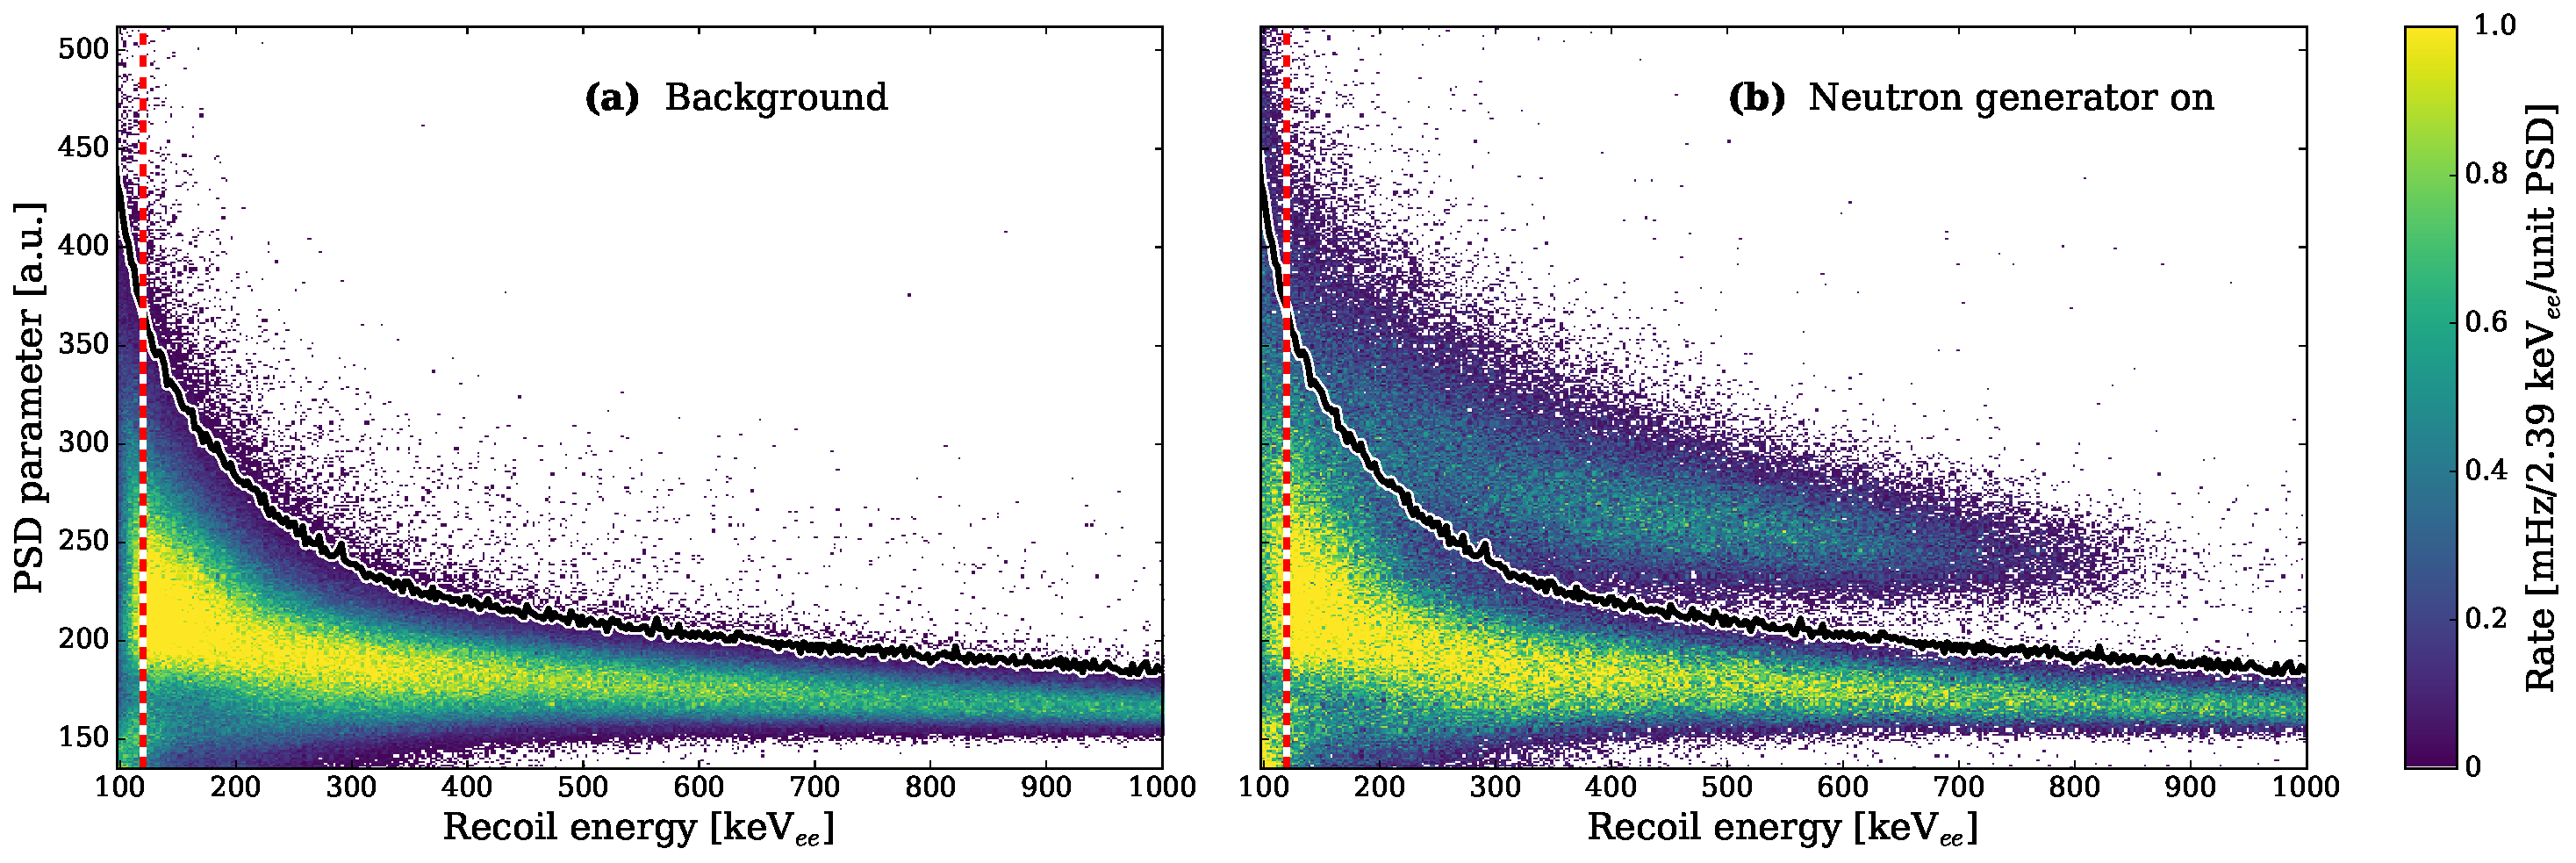
\includegraphics[width=1.0\textwidth]{figures/ng/hist2d_bg_and_fg}
    \caption{{\bf (a)} Data taken with the NE213 scintillator from a 21-hour background run and {\bf (b)} a 6-hour run with the neutron generator turned on, showing the pulse shape discrimination parameter as a function of recoil energy. A clear second neutron-induced band can be seen in the right panel. These recoils are selected using a $99\1{\%}$ background rejection cut in the pulse shape parameter, as indicated by the solid (black) line. The vertical dashed (red) line indicates the analysis threshold of $120\1{keV_{ee}}$ electron-equivalent energy.}\label{fig:hist2d}
\end{figure*}

\section{Neutron Energy Spectrum}\label{sec:en_spectrum}

We use the 2"$\times$2" cylindrical NE213 detector to determine the energy spectrum of the neutrons produced by the generator. Since this detector only measures the energy of the recoiling proton, there is no unique measurement of the incident neutron energy. Nevertheless two methods can be used to determine the incident neutron energy spectrum. Both require knowledge of the response function of the scintillator, which is simply a matrix that gives the distribution of the amount of scintillation light for a given incident neutron energy. We use a Monte Carlo-derived response function, which is based on measurements in monoenergetic and broad ns-pulsed neutron fields at PTB. The latter allows one to apply time-of-flight methods to select specific neutron energies~\cite{Dietze:1982,Klein:2002,Zimbal:2006}.

If the initial neutron energy spectrum is known, the observed recoil spectrum can  be calculated from the convolution of this response function with the incident spectrum, as we show in section~\ref{sec:convolution}. Alternatively, the observed recoil spectrum can be deconvoluted with the help of the response function in order to extract the incident neutron spectrum, as we do in section~\ref{sec:deconvolution}. The results that we obtain from both methods are in good agreement with each other.

\subsection{Data Selection}\label{sec:ng_data_selection}

The two parameters available for each event in the NE213 scintillator are the pulse height, which increases with the nuclear recoil energy, and the Zero Crossing Method pulse shape discrimination parameter~\cite{Alexander:1961}, which allows one to distinguish nuclear and electronic recoil events. Fig.~\ref{fig:hist2d} shows the histograms for both background data and data taken with the neutron generator turned on. The pulse height is converted to recoil energy (electronic recoil equivalent) by Monte Carlo-matching of a $^{207}$Bi gamma calibration spectrum. For proton recoil events, the nonlinear relation between proton recoil energy and the resulting signal amplitude, known as the light output function, is considered in the neutron response function data~\cite{Novotny:1997}.
A linear energy scale is assumed, which we verified to be correct at six energies ranging up to an electron-equivalent energy of $1546\1{keV_{ee}}$ using the Compton edges of the calibration sources $^{207}$Bi, $^{22}$Na and $^{137}$Cs.

We select neutron-induced events by cutting at the $99\%$ electronic recoil background rejection line in the pulse shape discrimination parameter space, as indicated in Fig.~\ref{fig:hist2d}. We subtract the background rate in the selected region by computing the number of events that pass the cut in the background data set and using the appropriate scaling for live-time.
We apply an energy threshold of $120\1{keV_{ee}}$ electron-equivalent energy in order to stay above energies where characteristic X-ray emission from the lead surrounding the NE213 detector starts to dominate.

\subsection{Cut Acceptance}

At low recoil energies, the pulse shape discrimination becomes less efficient. Due to $99\%$ background rejection criterion, for lower pulse heights an increasingly bigger fraction of neutron events does not fall in the selected region of neutron events. We calculate the fraction of neutron events passing this cut (the \emph{acceptance}) as a function of recoil energy as follows: for each energy bin, we subtract the live-time-normalized background data (Fig.~\ref{fig:hist2d}a) from the neutron generator data (Fig.~\ref{fig:hist2d}b) and fit a Gaussian to the resulting nuclear recoil distribution. The neutron acceptance, shown in Fig.~\ref{fig:acceptance}, is then taken as the area fraction of the Gaussian above the background rejection line. Also shown in the Fig.~\ref{fig:acceptance} is a smoothed interpolation that we use in the calculations that follow. We calculate the uncertainty on the acceptance by changing the fit parameters of the Gaussian within their uncertainty and re-computing the resulting acceptance.

\begin{figure}[!htbp]
\centering
    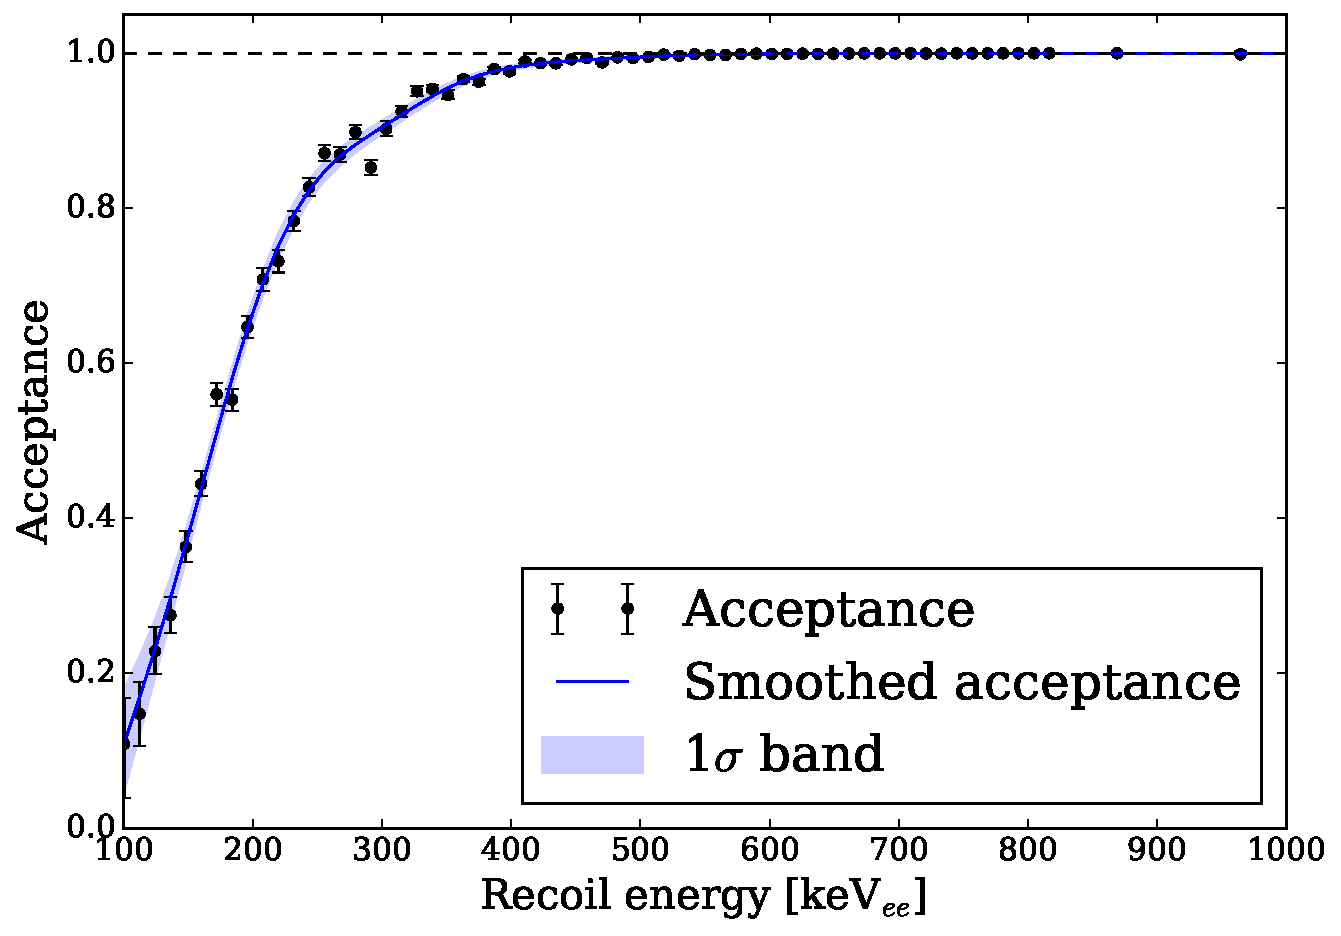
\includegraphics[width=\textwidth]{figures/ng/acceptance}
    \caption{The acceptance of the pulse shape cut (shown in Fig.~\ref{fig:hist2d}) as a function of energy. The Gaussian fraction above the pulse shape cut is shown by the (green) data points. The two points at the highest recoil energies are calculated with a wider bin width due to low statistics in the neutron band at these energies. The (blue) solid line is a lowpass-filtered interpolation of those data points. The $1\sigma$ uncertainty band on this acceptance is also shown (shaded blue).}
    \label{fig:acceptance}
\end{figure}

\subsection{Convolution}\label{sec:convolution}

The initial neutron energy spectrum in the neutron generator fusion region, calculated as described in section~\ref{sec:initialneutronspectrum}, is shown in Fig.~\ref{fig:incident_spectrum}. As can be seen, a plasma fusion generator as used here does not produce a truly monoenergetic neutron spectrum. Due to the dependence of the fusion cross section on the neutron emission angle relative to the momentum of the incident deuteron, the spectrum shows two peaks at $2.22\1{MeV}$ and $2.72\1{MeV}$ in the lab frame, corresponding to emission angles of $180\degree$ and $0\degree$, respectively.

Neutrons from this spectrum are propagated from the fusion region using GEANT4. The resulting neutron energy spectrum at the NE213 detector position is also shown in Fig.~\ref{fig:incident_spectrum}, where we normalized the spectra to the energy range from $2.2 - 2.7\1{MeV}$ for ease of comparison. The most significant impact to the neutron energy spectrum comes from scattering in the cooling water that surrounds the neutron generator fusion chamber. This causes the long tail towards lower energies and gives rise to the asymmetric peak structure.

\begin{figure}[!htbp]
\centering
    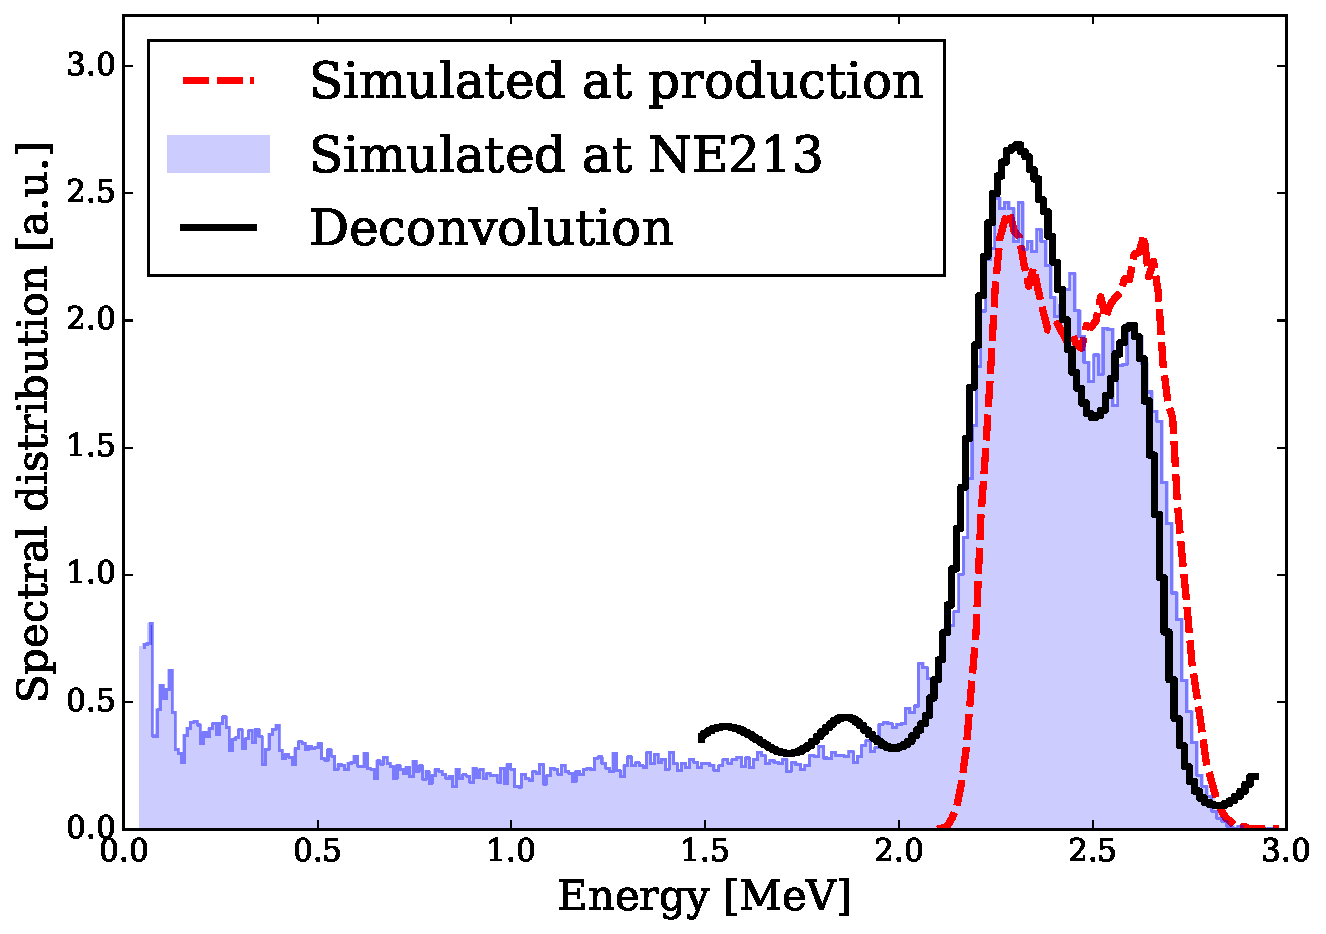
\includegraphics[width=\linewidth]{figures/ng/mc_spectrum}
    \caption{Shown are the simulated neutron spectrum in the neutron generator fusion region (red dashed line) and the resulting simulated spectrum at the NE213 detector (blue shaded histogram). Also shown is the result of the deconvolution of our data (black solid line), which is discussed in section~\ref{sec:deconvolution}. All spectra are normalized to the region $2.2 - 2.7\1{MeV}$ for ease of comparison.}\label{fig:incident_spectrum}
\end{figure}

We calculate the expected pulse height spectrum observed by the NE213 detector from the incident Monte Carlo-derived neutron energy spectrum. To this end, we apply the response function described earlier and use the data-derived acceptance function (Fig.~\ref{fig:acceptance}) to correct for acceptance losses at low pulse height energies. We normalize the expected pulse height spectrum to the observed data using a $\chi^2$-minimization in the energy range $(120-900)\1{keV_{ee}}$ electron-equivalent energy, where the upper limit of the considered energy range is placed at the point where signal and background rates become comparable. The result of this normalization is shown in Fig.~\ref{fit_with_acc} with its $1\sigma$ uncertainty, and the residuals. We find good agreement between the expected and observed distributions, validating the assumed energy spectrum of produced neutrons shown in Fig.~\ref{incident_spectrum}. A closer inspection of the residuals of the minimization indicates that our nuclear recoil acceptance may be slightly underestimated below $350\1{keV_{ee}}$.

In addition to the data selection method outlined in section~\ref{sec:ng_data_selection}, we repeated the analysis with no selection on the pulse shape discrimination parameter. The pulse height spectrum from the neutron generator is in this case computed by subtracting the background spectrum from the spectrum taken with the neutron generator turned on. Since this method requires no acceptance correction, it can be used as a cross-check of the cut-based analysis, however, with larger statistical uncertainty from the increased number of bins. Any gamma radiation caused by neutrons or Bremsstrahlung is ignored in this approach. By comparing the gamma-induced band for the neutron generator and background runs, we estimate that this contributes $<10$\% to the number of events between $300$ and $800\1{keV_{ee}}$. We find that the data selected by this simple background subtraction is consistent with the cut-based analysis if this effect is considered. % \lesssim?

\begin{figure}[!htbp]
\centering
    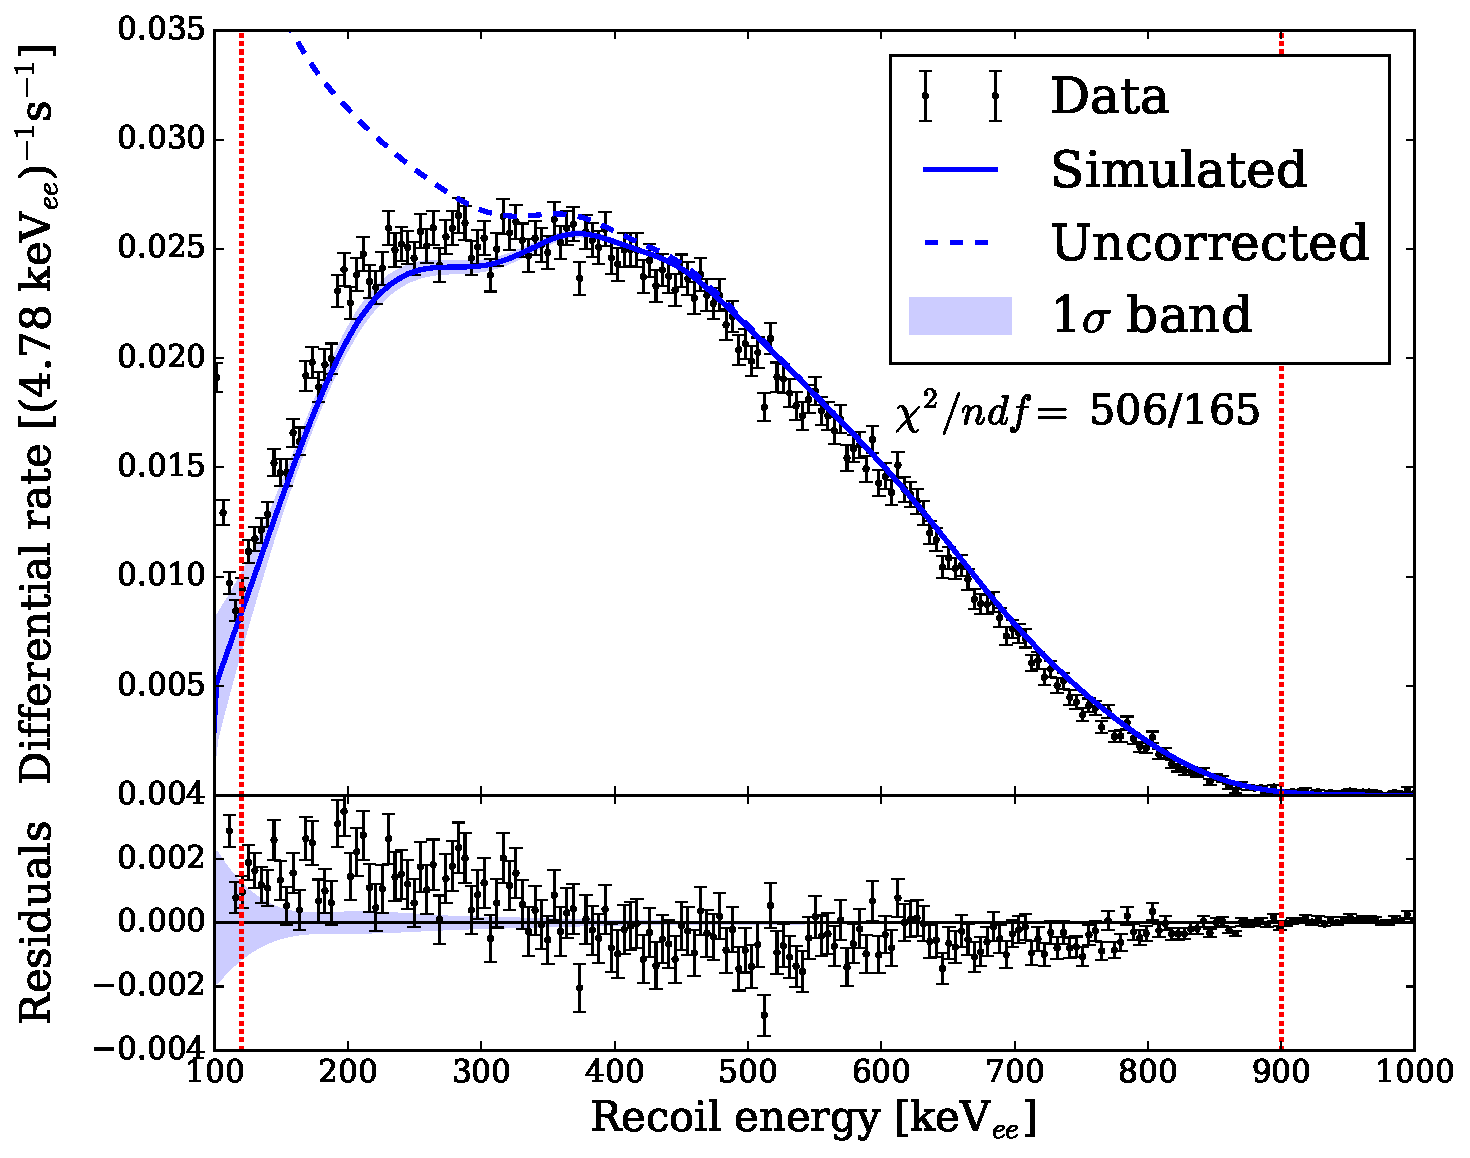
\includegraphics[width=\linewidth]{figures/ng/fit_with_acc_r}
    \caption{The observed background-rejected energy spectrum (green data points) together with the normalized expected distribution from simulation (solid blue line). The energy range considered for the normalization is indicated (red dotted lines). The reduced $\chi^2$ of the fit is 3.07. An indication of the effect of the acceptance correction can also be seen (dashed line). The (light blue) band around the simulated distribution indicates the uncertainties from the acceptance function. The bottom panel shows the residuals between data and simulation after normalization. }\label{fig:fit_with_acc}
\end{figure}

\subsection{Deconvolution}\label{sec:deconvolution}
We determine the neutron spectrum through a deconvolution of  the observed nuclear recoil pulse height spectrum. For this analysis, we use the same data selection, background treatment and acceptance correction as in section \ref{sec:convolution}, but restrict the energy range to $350\1{keV_{ee}}-950\1{keV_{ee}}$.
The main purpose of the deconvolution is an independent confirmation of the expected line shape of the $2.45\1{MeV}$ neutron peak resulting from reaction kinematics and Monte Carlo modeling of the setup. The recorded pulse height events below $350\1{keV_{ee}}$ do not contribute to this information but cause instabilities in the deconvolution process due to non-perfect neutron-gamma separation and systematic limitations in the precise determination of the response function in this energy range.

We use a combination of the GRAVEL~\cite{Matzke:1994} and MAXED~\cite{Reginatto:2002} deconvolution codes, with GRAVEL providing the starting values that are then used for further refinement using the MAXED code. The allowed neutron energy range for this analysis is $1.49 - 2.92\1{MeV}$, corresponding to the light output of the selected pulse height range.

The neutron spectrum obtained from this deconvolution is shown in Fig.~\ref{incident_spectrum}. In agreement with the Monte Carlo simulation, this deconvolved spectrum shows a double-peaked structure around $2.4\1{MeV}$, rather than a purely monoenergetic neutron emission. At low energies $(<2.0\1{MeV})$, an oscillatory feature appears. However, only a small fraction of the low-energy neutrons can induce a signal above our analysis threshold of $350\1{keV_{ee}}$. Consequently, small changes in the analysis (such as the considered energy range or data selection criteria) result in significant changes to the spectral shape below $2.0\1{MeV}$. We thus do not consider this neutron energy range any further. A small contribution is seen at the highest allowed energies $(>2.8\1{MeV})$. As discussed in the next section, we attribute this contribution to the presence of high-energy neutrons from deuterium-tritium fusion.

\subsection{High-Energy Neutrons} \label{sec:he_neutrons}

Upon inspection of the NE213 nuclear recoil data at high ($>1000\1{keV_{ee}}$) energies, we observed a secondary population at energies above those expected from $2.45\1{MeV}$ deuterium-deuterium neutrons. We attribute these high-energy recoils to deuterium-tritium fusion, produced in the neutron generator as a result of the reactions
\begin{eqnarray}
{}^2\mathrm{D} + {}^2\mathrm{D} \rightarrow \mathrm{p}\, + &\!\!\!\!{}^3\mathrm{T}\!\!\!\!& \label{eq:t_production_reaction} \\
&\!\!\!\!^3\mathrm{T}\!\!\!\!& + {}^2\mathrm{D} \rightarrow {}^4\mathrm{He} + \mathrm{n}(14.1\1{MeV}).
\end{eqnarray}
Reaction~\eqref{eq:t_production_reaction} is equally likely to occur at $50\1{keV}$ as the main neutron producing reaction~(Eq~\eqref{eqn:main_reaction})~\cite{Huba:2013}. Since the deuterium-tritium fusion reaction has a cross section that is more than two orders of magnitude higher than that of deuterium-deuterium fusion, even a small tritium contamination can give a non-negligible amount of $14.1\1{MeV}$ neutrons in the spectrum.

To test this hypothesis, we rebin the recoil energy spectrum as shown in Fig.~\ref{fig:he_spec}. Due to the low statistics, the deconvolution code is prone to reconstruction artifacts. We therefore only use the convolution method, with $14.1\1{MeV}$ neutrons as the initial spectrum originating in the neutron generator fusion volume. Again, scatters in surrounding materials were taken into account by propagating the neutron spectrum to the detector in GEANT4. As the separation between the electronic and nuclear recoil bands in the NE213 detector is excellent at these high recoil energies ($>1000\1{keV_{ee}}$), the acceptance is taken to be unity. The resulting simulated recoil spectrum is shown in Fig.~\ref{fig:he_spec}, scaled to data. We find an excellent agreement between data and simulation, confirming our hypothesis of deuterium-tritium fusion taking place in the generator.

\begin{figure}[!htbp]
\centering
    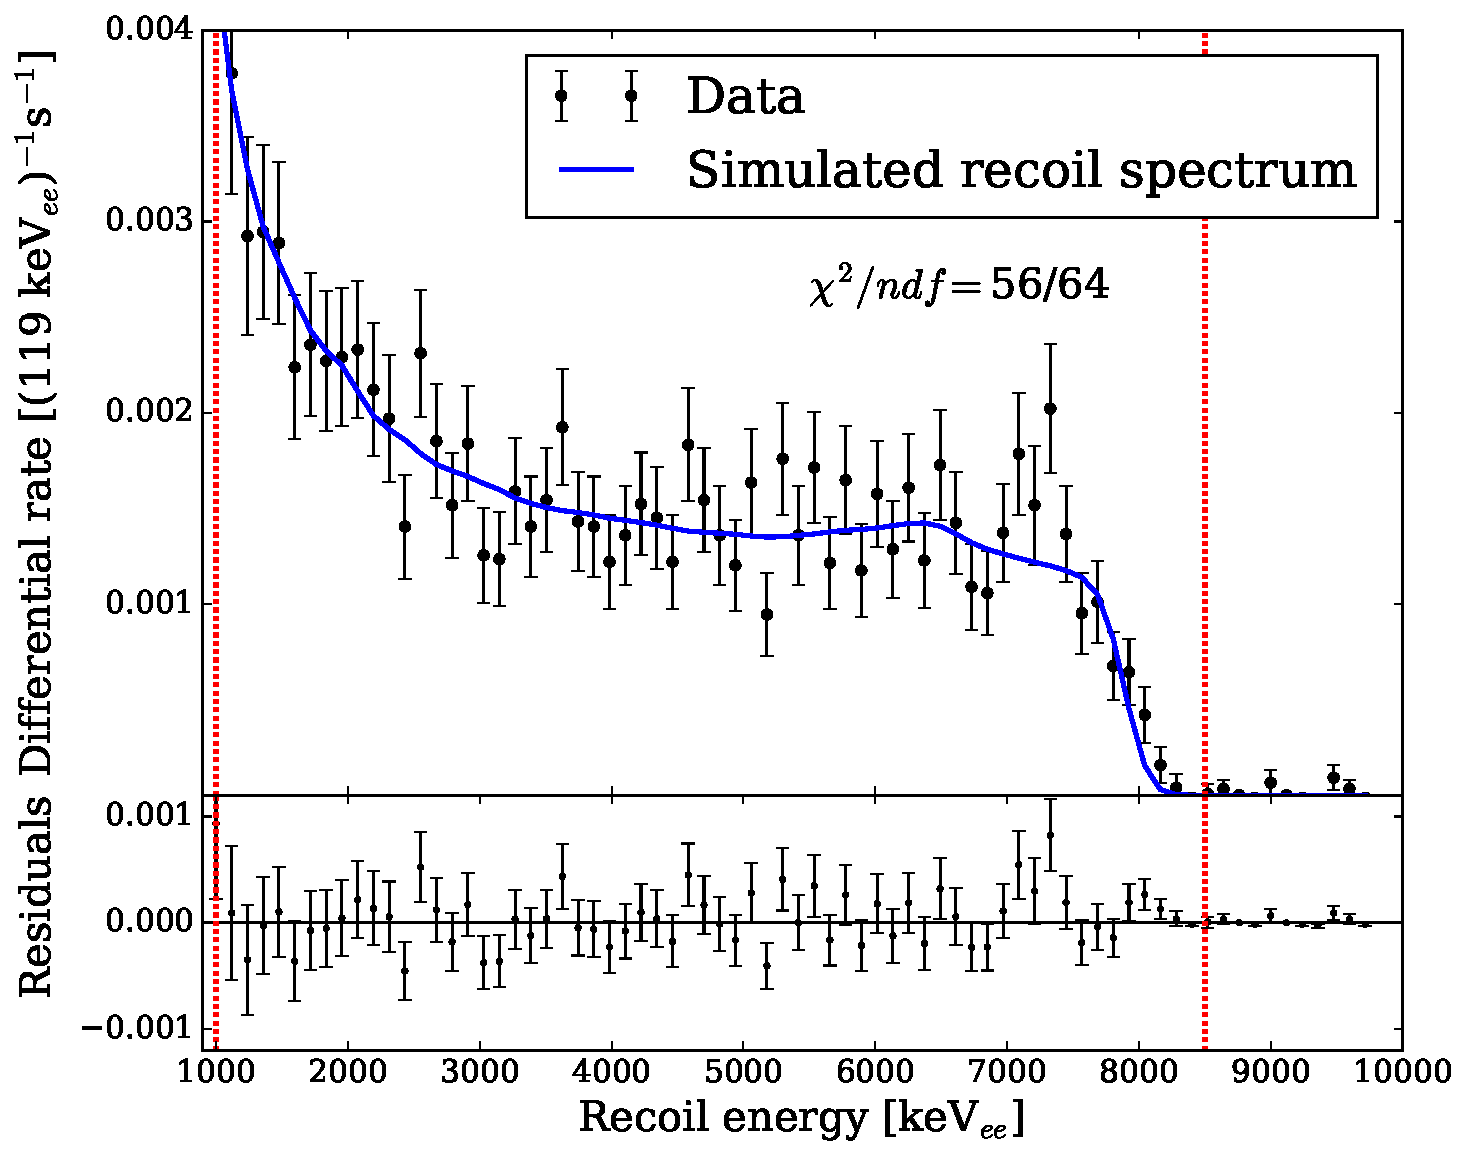
\includegraphics[width=\linewidth]{figures/ng/he_spec}
    \caption{The observed spectrum at high recoil energies (green data points) together with the normalized distribution expected from $14.1\1{MeV}$ neutrons from deuterium-tritium fusion (solid blue line). Again, the energy range considered for the normalization is indicated (red dotted lines) and residuals from the normalization are shown in the bottom panel. The reduced $\chi^2$ of the fit is 0.875.}\label{fig:he_spec}
\end{figure}

For a quantitative analysis, we calculate the ratio of the deuterium-tritium neutron flux to the flux of neutrons integrated between $2.0$ and $2.8\1{MeV}$ in the deconvoluted energy spectrum, taking into account the energy-dependent response of the NE213 detector. We arrive at a total ratio of $(5.5 \pm  0.3)\%$. This is consistent with the yield expected from tritium produced during the operation of the neutron generator prior to the data taking presented here. To determine the ratio of deuterium-tritium neutrons to the flux of all neutrons from deuterium-deuterium fusion, we calculate the fraction of neutrons produced in the GEANT4 MC simulation with energies below $2.0\1{MeV}$. In total 37.34\% of the simulated neutrons have incident energies below $2.0\1{MeV}$ when they reach the detector. This is in agreement with the difference in flux measured by the NE213 detector and the Long Counter, discussed at the end of section~\ref{sec:flux}. We conclude that the total ratio of deuterium-tritium neutrons is $(3.5 \pm  0.2)\%$.

\section{Neutron Flux}\label{sec:flux}

\subsection{Relative Dependence}\label{sec:relativeflux}

Measurements were taken at Purdue University to measure the functional dependence of the neutron flux on the operational parameters of the neutron generator, namely the high voltage $V$ and the current $I$ applied to the cathode. High voltages were set to between $30\1{kV}$ and $52\1{kV}$, and currents were set to between $0.5\1{mA}$ and $1.1\1{mA}$. Measurements of the high voltage, current, and getter pump temperature were collected in one minute intervals. Three EJ301 organic liquid scintillator detectors were used to measure the neutron flux. Because this experiment was conducted in a small lab, the resulting backscattering of neutrons from the walls prevents us from using this data to determine the absolute neutron flux. This does not however prevent measurement of the relative functional dependence on $V$ and $I$.

A total of 107~datasets with a combined live-time of 55.3~hours were collected with the detectors level with the neutron-producing region of the generator. We have previously studied and improved upon the pulse shape discrimination using the EJ301 detectors. That work allows us to reduce the recoil energy threshold for this analysis to $50\1{keV_{ee}}$ electron-equivalent energy at 99.5\% electronic recoil rejection, using a Laplace transform-based pulse shape discrimination parameter (Ref.~\cite{Lang:2016xks}, also Chapter~\ref{ch:psd}).

We obtain a rate of nuclear recoils passing this rejection cut and fit a function of the form
\begin{equation} \label{eq:rate}
F(V,I) = aV^b I^c.
\end{equation}

As the neutron flux depends strongly on the applied high voltage, which varied during a run by up to several hundred volts, the voltage measurements are averaged together for each run via the expression

\begin{equation}
\langle V \rangle = \left(\frac{1}{n}\sum\limits_{i=0}^n V_i^p \right)^{1/p}
\end{equation}
The exponent $p$ is determined to be 3.33 through an iterative process where a value is chosen, the functional dependence is calculated from the data, and the resulting voltage exponent used to re-average the voltage measurements. This was repeated until the values converged. Typical variations in the applied current were of order $\n{\mu A}$. Since the relative variations are much smaller and the flux depends only weakly on current, no averaging process was required for the current.

To estimate systematic uncertainties in the values of $b$ and $c$, we investigate variations of the selection criteria and also compare the results from the three different detectors. We find the results to be robust against changes in the $50\1{keV_{ee}}$ energy threshold requirement as well as against variations in the exponent $p$ used when averaging high voltage measurements.

Due to scattering of neutrons from the walls, the value found for $a$ is not an accurate measurement of the overall scaling of the function, but we find $b=3.32\pm0.14$ and $c=0.97\pm0.01$. Figure~\ref{fig:fluxandfit} shows the normalized measured neutron rates as a function of cathode high voltage, at fixed current.

\begin{figure}[!htbp]
\centering
    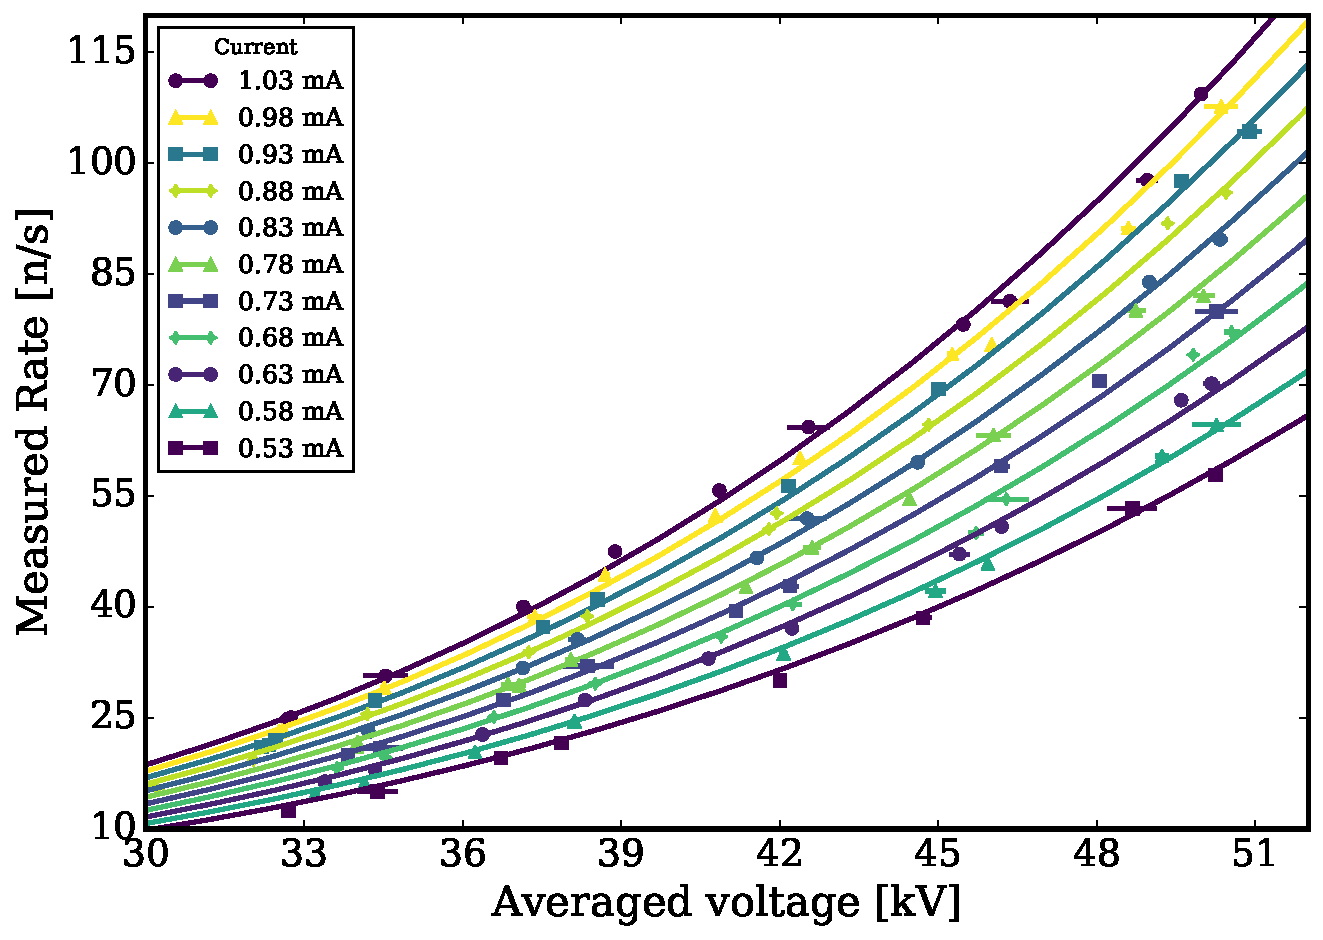
\includegraphics[width=\columnwidth]{figures/ng/fig_fluxandfit_v2_0}
    \caption{Measurements of the relative neutron flux produced by the neutron generator at Purdue University for various values of the operational parameters (cathode high voltage and current). The current at which each measurement was taken is represented by the color of the data point. The flux from the functional fit was found to be proportional to $(\n{Voltage})^{3.32}$ and $(\n{Current})^{0.97}$. The solid lines represent the predicted neutron flux as a function of cathode high voltage, at a fixed current.}\label{fig:fluxandfit}
\end{figure}

\subsection{Absolute Flux}

To measure the absolute neutron flux, a similar measurement was performed at the PTB, where the large experimental hall resulted in significantly less environmental scattering of neutrons. The Long Counter was used as the detector, placed at a distance of $1.569\1{m}$ from the neutron generator, as measured to the front face of the detector. A total of 10~datasets were collected at different high voltage and currents settings over a wider range than measured at Purdue. The same fitting procedure described above was applied, resulting in $b = 3.31 \pm 0.08$, and $c = 1.00 \pm 0.02$, consistent with the Purdue measurements.

We use the energy-dependent Long Counter~\cite{Roberts:2004} response, taking into account neutron contributions from both deuterium-deuterium and deuterium-tritium fusion, to correct the measured neutron flux for the space angle covered by the detector. Additionally we correct for the residual environmental scattering from the experimental hall. Furthermore, we also take into account the anisotropic neutron emission presented in the next section. We thus find for the absolute deuterium-deuterium neutron output outside of the neutron generator in the full $4\pi$ space angle (see equation~\eqref{eq:rate}) $a = (8.0 \pm 0.6)\times10^{-2}\1{s^{-1}}$ with $V$ in kV and $I$ in mA. Given the determined values of $a$, $b$ and $c$, the measurements of neutron flux performed here span a range from $7.8\times 10^3$ to $1.16\times 10^5\1{s^{-1}}$. We expect that the functional dependence of the rate on the operational parameters is valid for neutron fluxes higher than those measured in this work.

As a cross check for consistency, we compare the measured neutron flux in the NE213 detector and the Long Counter. For the Long Counter we use data collected at a polar angle of $90\degree$ and an effective radial distance of $1663\1{mm}$. Here we have included the distance to the effective center of the Long Counter, which is $94\1{mm}$ behind the front face of the detector. The neutron generator was set to $2.0\1{mA}$ and $50\1{kV}$, resulting in a measured neutron flux in the Long Counter of $(0.247 \pm 0.022)\1{cm^{-2}\,s^{-1}}$. We compare this to data collected with the NE213 detector at an effective radial distance of $892\1{mm}$ (which includes the distance to the effective center of the NE213 detector of $27\1{mm}$) and a polar angle of $90\degree$. This yielded a measured neutron flux of $(0.643 \pm 0.064)\1{cm^{-2}\,s^{-1}}$ between $2.0$ and $2.9\1{MeV}$. Taking into consideration the full neutron energy spectrum (discussed in section~\ref{sec:he_neutrons}) the total flux is $(1.06 \pm 0.11)\1{cm^{-2}\,s^{-1}}$. This value is then corrected for the difference in radial distances between the two detectors and scaled for the different current settings using equation~\eqref{eq:rate}. The comparable neutron flux from the NE213 detector is thus determined to be $(0.246 \pm 0.025)\1{cm^{-2}\,s^{-1}}$.

\section{Angular Emission of Neutrons}\label{sec:angular}

The internal geometry of the neutron generator cylinder is azimuthally symmetric, but not along its axis. We therefore assume that the flux of neutrons is independent of azimuthal angle, and measure the neutron flux as a function of polar angle (compare Fig.~\ref{fig:ptb_coordinates}). An angular scan was performed in steps of $10\degree$ ranging from $10\degree$ to $180\degree$ using the Long Counter. For these measurements, the neutron generator was operated at a high voltage of $50\1{kV}$ and a current of $2\1{mA}$, and we collected approximately 1000~neutron counts for each measurement.

\begin{figure}[!htbp]
\centering
    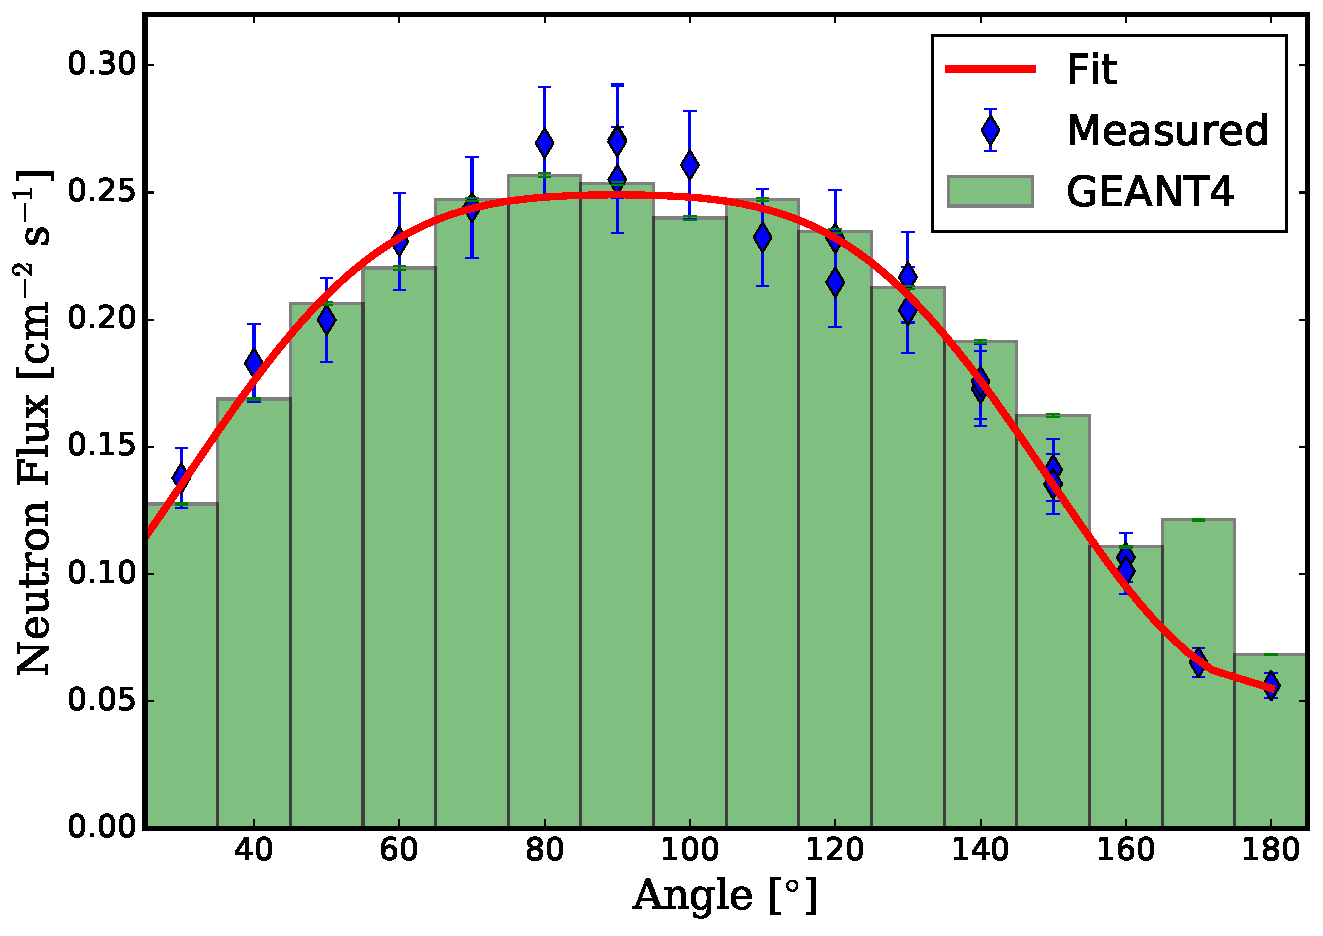
\includegraphics[width=\columnwidth]{figures/ng/fig_angle_scan}
    \caption{Measured neutron flux as function of polar angle. Data taken with the the Long Counter is shown (blue diamonds) together with the angular neutron flux dependence predicted by a detailed GEANT4 simulation of the neutron generator (green bars). A fourth order polynomial fit to the data is shown as well (red line), parametrizing the measured dependence.}
    \label{Fig:Angle_Scan_Match}
\end{figure}

Data taken with both the Long Counter and the EJ301 detector at PTB were corrected for the neutron flux that was produced, given the average high voltage and current, as discussed previously. After correction, the measured number of neutrons in the EJ301 detector (which was held at a constant angle throughout) was found to have a standard deviation of $7.5\,\%$ across the angular scan measurements. The neutron flux at the location of the Long Counter, shown in Fig.~\ref{Fig:Angle_Scan_Match}, was calculated from the count rate using the energy-dependent response of the Long Counter~\cite{Roberts:2004}.

A fourth order polynomial, of the form $F(\cos\theta)=A+B\cos^{2}\theta+C\cos^{4}\theta$, is fitted to the Long Counter measurements in order to parametrize the angular dependence of the neutron flux. The resulting fit parameters are $A=(0.237\pm0.006)\1{cm^{-2}\,s^{-1}}$, $B=(-0.051\pm0.028)\1{cm^{-2}\,s^{-1}}$ and $C=(-0.130\pm-0.025)\1{cm^{-2}\,s^{-1}}$.

%F(\theta) = \frac{(36.4 \pm 0.9)}{\sqrt{2 \pi} (52 \pm 1)} e^{\frac{-(\theta+(1.46 \pm 1.5))^2}{2 (52 \pm 1)^2}}
We simulate the expected angular dependence using the detailed neutron generator setup in GEANT4. The Long Counter is placed at the correct distance and angle of each respective measurement. The EJ301 detector is also present in the simulation to account for any scattering off of the EJ301 cell into the Long Counter as the latter is placed closer to the EJ301 cell for large polar angles. At each angle we simulate $10^8$~neutrons distributed homogeneously throughout the cathode and emitted isotropically with the energy spectrum previously calculated. The GEANT4 Monte Carlo data sets are expressed in terms of a neutron flux, using the energy-dependent response function of the Long Counter derived from GEANT4. The resulting simulated angular dependence is also shown in Fig.~\ref{Fig:Angle_Scan_Match}.

The simulation results agree well with data. We conclude that the measured angular emission spectrum is well described by isotropic production of neutrons within the volume of the cathode field cage, with any angular variations being a result of the interior geometry and composition of the neutron generator.

\section{Conclusions}

We have performed the first characterization of the neutron flux produced by a deuterium-deuterium plasma fusion neutron generator. Our interest lies in the application of this generator as a nuclear recoil calibration source for a sensitive dark matter scattering experiment~\cite{Aprile:2015uzo}. For this application, accurate knowledge of both the energy spectrum and the absolute flux are mandatory.

We found that the energy spectrum is not strictly monoenergetic, but contains two peaks at $2.22\1{MeV}$ and $2.72\1{MeV}$. These are understood to be caused by the dependence of the neutron energy on the neutron emission angle relative to the momentum of the incident deuteron. Running this generator produces small quantities of tritium that resulted in a measurable flux of $14.1\1{MeV}$ neutrons due to deuterium-tritium fusion in the plasma. These deviations from an ideal, monoenergetic spectrum will have to be taken into account in any measurement using deuterium-deuterium generators that aims to use the energy information of the incident neutron.

We have also characterized the dependence of the absolute neutron flux on the applied high voltage and current, as well as the dependence of the emitted neutron flux on polar angle. Monte Carlo simulations showed that the angular distribution of the neutron flux is affected by transmission of neutrons through the generator housing. The measured angular distribution is consistent with an isotropic neutron source inside the generator. Taken together, knowledge of this parametrization will allow us to break the degeneracy in calibration between decreasing acceptances of a detector and varying flux output from the neutron source~\cite{Aprile:2013teh}.

We have developed a Monte Carlo simulation of the neutron generator characterized in this work, which accurately predicts the emitted neutron flux. The simulation is able to reproduce both the measured angular emission spectrum and energy of emitted neutrons. Thus we have a predictive model of the behavior of the neutron generator as a nuclear recoil calibration source for other applications.

% rn220 source
% Rn source paper, v1.0

\chapter{Characterization of the Rn-220 source}\label{ch:rn220}

\paragraph{Abstract} The increased size of XENON1T renders external $\gamma$ sources insufficient for proper calibration of the fiducial volume. To solve this problem, we developed a novel source of $^{220}$Rn that can be dissolved into the xenon target. Radiation from the daughter products provide an effective calibration of the entire active volume. We measured the emanation of potential long-lived contaminants $^{228}$Th and $^{224}$Ra released by the source and verified that it does indeed mix throughout a xenon detector. The results were published as Lang et al, JINST 11(04):P04004, 2016.

\section{Introduction}

Various low-background experiments are searching for rare events such as neutrinoless double-beta decay~\cite{Pandola:2014naa} or dark matter scatters~\cite{Undagoitia:2015gya}. Time projection chambers (TPCs) using liquid noble elements such as argon and xenon are at the forefront of these investigations~\cite{Albert:2015eem,Aprile:2015uzo,Akerib:2015rjg,Amaudruz:2014nsa,Calvo:2015uln,Agnes:2015ftt}. As these detectors become large, new challenges arise in accurately calibrating their response throughout the detection volume. For example, the XENON1T detector~\cite{Aprile:2015uzo} is a TPC $1\1{m}$ in diameter and in height, much larger than e.g. the $70\1{mm}$ mean free path of the $1.3\1{MeV}$ $\gamma$ from $^{60}$Co. Thus, calibration of the entire fiducial volume with external sources is no longer feasible.

One solution is to directly mix a radioactive isotope into the liquid noble element. In liquid xenon, $^{83m}$Kr has been used~\cite{Akerib:2017eql} to achieve a low-energy line calibration throughout the detector, as has $^{127}$Xe electron capture~\cite{Akerib:2017hph}. Tritiated methane has been used as a low-energy beta source~\cite{Akerib:2015wdi}, as well as $^{14}$C. While these sources has the advantage that many or all decays are in the low-energy range interesting to a dark matter search, they suffers from the disadvantage that the activity does not decay by itself but must be extracted from the liquid target by a hot zirconium getter in a xenon recirculation loop~\cite{Akerib:2015wdi}. This introduces an additional time constant that will get longer as the size of these detectors increases.

Here, we study a source containing $^{228}$Th~that emanates $^{220}$Rn~($T_{1/2}=56\1{seconds}$), which in turn can be mixed into the liquid target. The $^{220}$Rn~decay chain is versatile, producing $\alpha$-, $\beta$-, and $\gamma$-radiation that makes this source interesting for a wide range of applications: The source is the ideal calibration source for intrinsic $^{222}$Rn backgrounds that are notoriously difficult to control in low-background experiments. (2) High-energy alphas~\cite{Albert:2015vma,Aprile:2017fhu} and $^{212}$Bi/$^{212}$Po decays~\cite{Bellini:2012qg} can be used to accurately understand intrinsic backgrounds. The relatively short half-life of $^{216}$Po (145~ms) allows for the measurement of currents or liquid flows within the bulk of the detector volume. Using position reconstruction algorithms that yield the positions of the decays of $^{220}$Rn~and $^{216}$Po together with the time difference between these two decays, allows for a measurement of the drift velocity of polonium ions~\cite{Albert:2015vma}. Thus, currents within the bulk of the detector can be mapped to identify possible dead regions that do not participate in the recirculation of the active volume through purification systems. Additionally, the high-energy $\alpha$ lines can be used to probe regions in a detector with poor light or charge collection efficiency. Further, the $^{208}$Tl decay produces a $2.6\1{MeV}$ $\gamma$-line, very close to the Q-value of $^{136}$Xe double-beta decay. This line will be accompanied by the $\beta$ energy and usually by simultaneous $\gamma$-lines (mostly $580\1{keV}$), which results in steps in the calibration spectrum (e.g. at $\approx 3.2\1{MeV}$) above the $^{136}$Xe Q-value. Finally, $\beta$-decays of the chain that go to the ground state can be used to calibrate the low-energy response of dark matter detectors. While the high Q-value of the $^{212}$Bi $\beta$-decay (2.2~MeV) and short life-time of the daughter $^{212}$Po (300~ns) render that decay unsuitable for this purpose, the $\beta$-decay of $^{212}$Pb~(12.3\% branching ratio to ground state, Q-value 560~keV) is very suitable for this task, as shown in Figure~\ref{fig:pb212spectrum}.

\begin{figure}[htbp]
\centering
    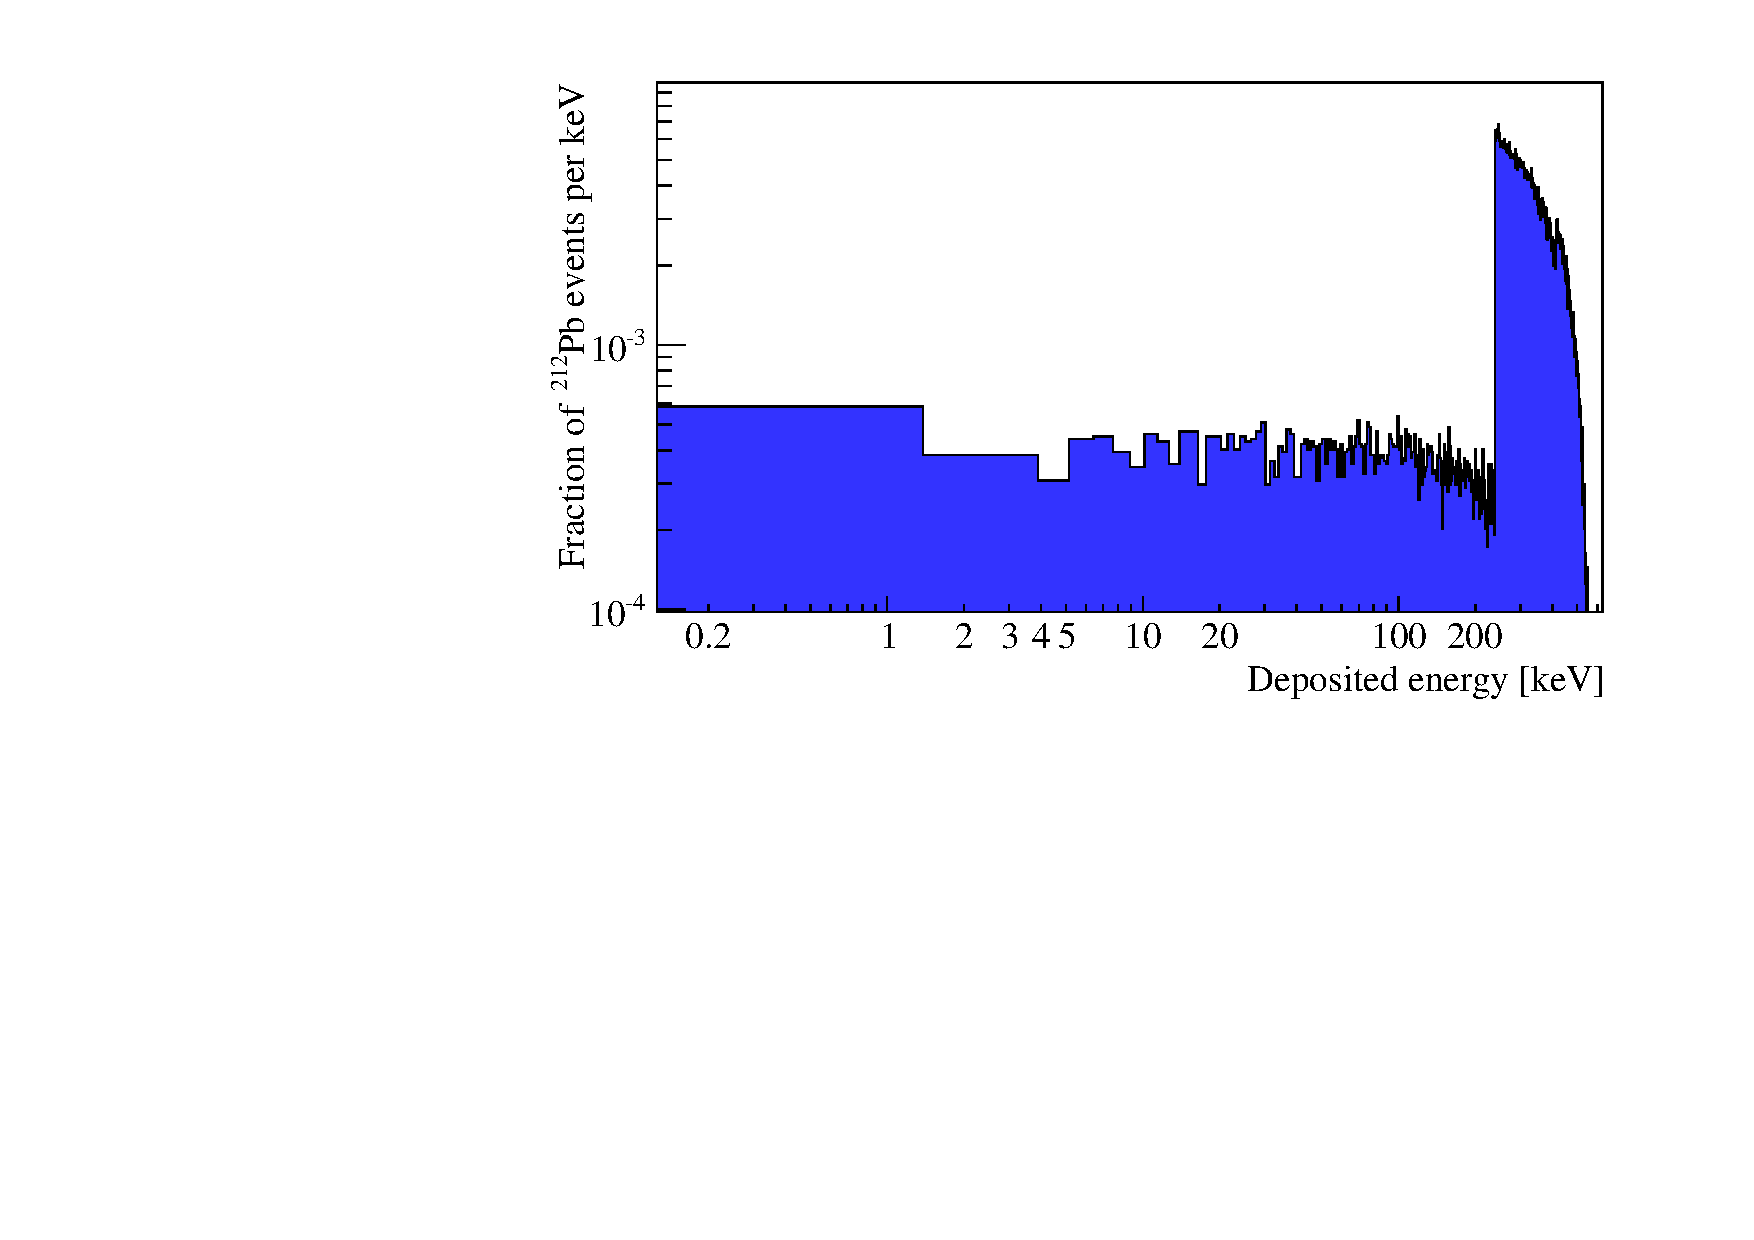
\includegraphics[trim = 5 0 50 15, clip = true,width = 0.8\columnwidth]{figures/rnsource/pb212_spectrum}
    \caption{A simulation of the $\beta$-spectrum of $^{212}$Pb. The feature at 240 keV is due to decay modes with an associated $\gamma$ that adds to the energy observed in the decay.}\label{fig:pb212spectrum}
\end{figure}

A major advantage of our source is that the time scale of the $^{220}$Rn~decay chain is dominated by the relatively short half-life of $^{212}$Pb~($T_{1/2}=10.66\1{hours}$). Thus, the introduced activity can completely decay away within a few days, making this source useful even for the largest anticipated liquid detectors~\cite{Aalbers:2016jon,Akerib:2018lyp,Franco:2015pha}. As both $^{228}$Th~($T_{1/2}=1.9\1{years}$) and $^{224}$Ra~($T_{1/2}=3.6\1{days}$) have much longer half-lives, emanation of these isotopes from the source must be limited. Also, isotopic contaminations with $^{230}$Th in the $^{228}$Th source itself can lead to the emanation of $^{222}$Rn ($T_{1/2}=3.8\1{days}$) which has to be avoided.

Here, we use a variety of methods to derive limits on the release of long-lived isotopes, and demonstrate that these sources are suitable for the calibration of even next-generation low-background experiments. Open $^{220}$Rn~sources were produced by electroplating thorium nitrate, $\n{Th}(\n{NO}_3)_4$, onto the center of a $30\1{mm}$ diameter stainless steel disk in a bath of 1M nitric acid ($\n{HNO}_3$). A ring of width 2.5~mm around the edge of the disk was left for mounting purposes. The activity was $40\1{kBq}$ as of March, 2015. Each source is held in a small stainless steel vessel to attach it to a noble gas recirculation system using 1/2"~VCR piping, see figure~\ref{fig:th228source}.

\begin{figure}[htbp]
\centering
    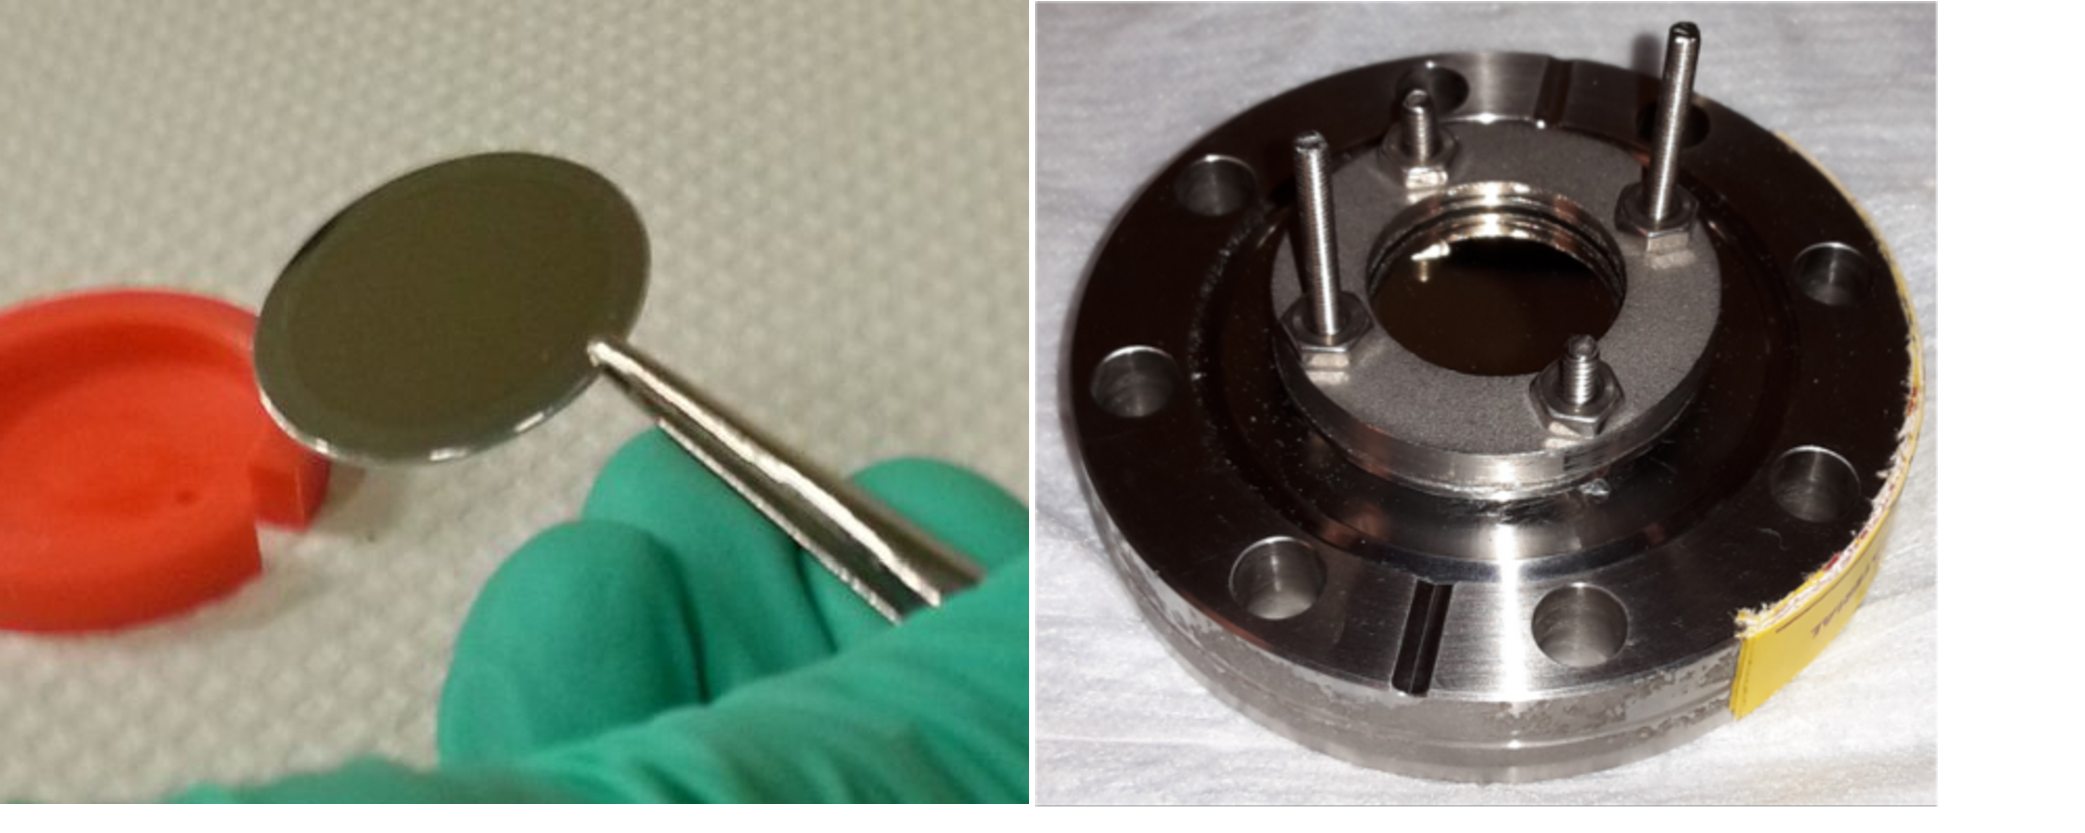
\includegraphics[trim = 5 10 50 0, clip = true,width = 0.8\columnwidth]{figures/rnsource/source_image}
    \caption{$^{228}$Th~is deposited onto a $30\1{mm}$ stainless steel disc (left). It is held in a simple emanation vessel (right) for mounting on a noble gas system.}\label{fig:th228source}
\end{figure}

\section{$\gamma$-Measurements of Filter Deposition}
\label{sec:tuv}

% TUV measurement
The source was tested
for the release of $^{224}$Ra~and $^{228}$Th~using a standard procedure. Nitrogen was flushed through the source vessel for 96 hours. A filter of type ML050/0 was mounted inline $18\1{cm}$ after the source, containing a filter paper on which any released radionuclides could be deposited. This filter paper was then tested for $\gamma$-activity with a high-purity germanium detector. A first measurement was made immediately after exposure, and a second measurement a week later, see Table~\ref{tab:tuv}.

\begin{table}[htb]
\centering
    \caption{Measurements of radionuclide release from the $^{220}$Rn~source collected in filter paper.}
    \label{tab:tuv}
    \renewcommand{\arraystretch}{1.2}
    \begin{tabular}[c]{|llcc|}
        \hline\hline
        \multicolumn{2}{|l}{Measurement} & 1 & 2 \\
        \multicolumn{2}{|l}{Time after exposure} & Immediate & 1 week \\
        \multicolumn{2}{|l}{Livetime} & $375\1{s}$ & $11500\1{s}$ \\ \hline
        \multirow{5}{*}{Activity/Bq}
        & $^{228}$Th & $<35$ & $<1.97$ \\
        & $^{224}$Ra & $<6$ & $<0.61$ \\
        & $^{212}$Pb & $87\pm11$ & $<0.07$ \\
        & $^{212}$Bi & $84\pm34$ & $<0.68$ \\
        & $^{208}$Tl & $28\pm5$ & $<0.07$ \\
        \hline\hline
    \end{tabular}
\end{table}

Both the exposure time and the time between measurements are significant compared to the half-life of $^{224}$Ra. We account for both the decay during these intervals as well as the production of $^{224}$Ra~from the decay of $^{228}$Th. The week between the two measurements is more than 15 half-lives of $^{212}$Pb, hence any recorded activity of its daughters $^{212}$Bi or $^{208}$Tl in the second measurement would have been from the decay of $^{224}$Ra, not any initial population of $^{212}$Pb. We use the lowest measurement (here, $^{212}$Pb) to constrain the release of $^{224}$Ra~from the source to $<0.43\1{atoms/s}$ and that of $^{228}$Th~to or $<22\1{atoms/s}$. Scaling these values for the activity of the source yields a stray emanation of $<0.66\1{atoms/min/kBq}$ $^{224}$Ra~and $<34\1{atoms/min/kBq}$ $^{228}$Th. We choose these units (atoms/min/kBq) to account for the decay of the sources over the time the various measurements were made, and to allow comparisons between the sources.

The obvious limitation of this measurement is that there may have been radium or thorium released by the source but not caught by the filter, in which case the given limits must be scaled by the efficiency of the filter. Additionally, any thorium or radium plated out on the pipes connecting the source vessel and the filter would not show up in this measurement.

% Jochen's measurements
A similar but more sensitive experiment was performed by pumping nitrogen at 1 standard liter per minute (slpm) for 9 days in a closed loop through the $^{220}$Rn~source vessel. The source was followed by a MILLEX-FG 50 filter at a distance of 8~cm, containing a $0.2\1{\mu m}$ PTFE filter membrane. The exposure time brought any released $^{224}$Ra~nearly into equilibrium on the filter and gave potential $^{228}$Th~more time to deposit itself. After exposure, the filter membrane was tested for $\gamma$-activity with high-purity germanium detectors~\cite{Budjas:2007,Budjas:2009}. A spectrum of these measurements is shown in figure~\ref{fig:gammaspectrum}. A simulation of the germanium crystal detector geometry performed in GEANT4~\cite{Geant4} indicated an efficiency of 6.5\% at 240 keV.

\begin{figure}[htb]
\centering
    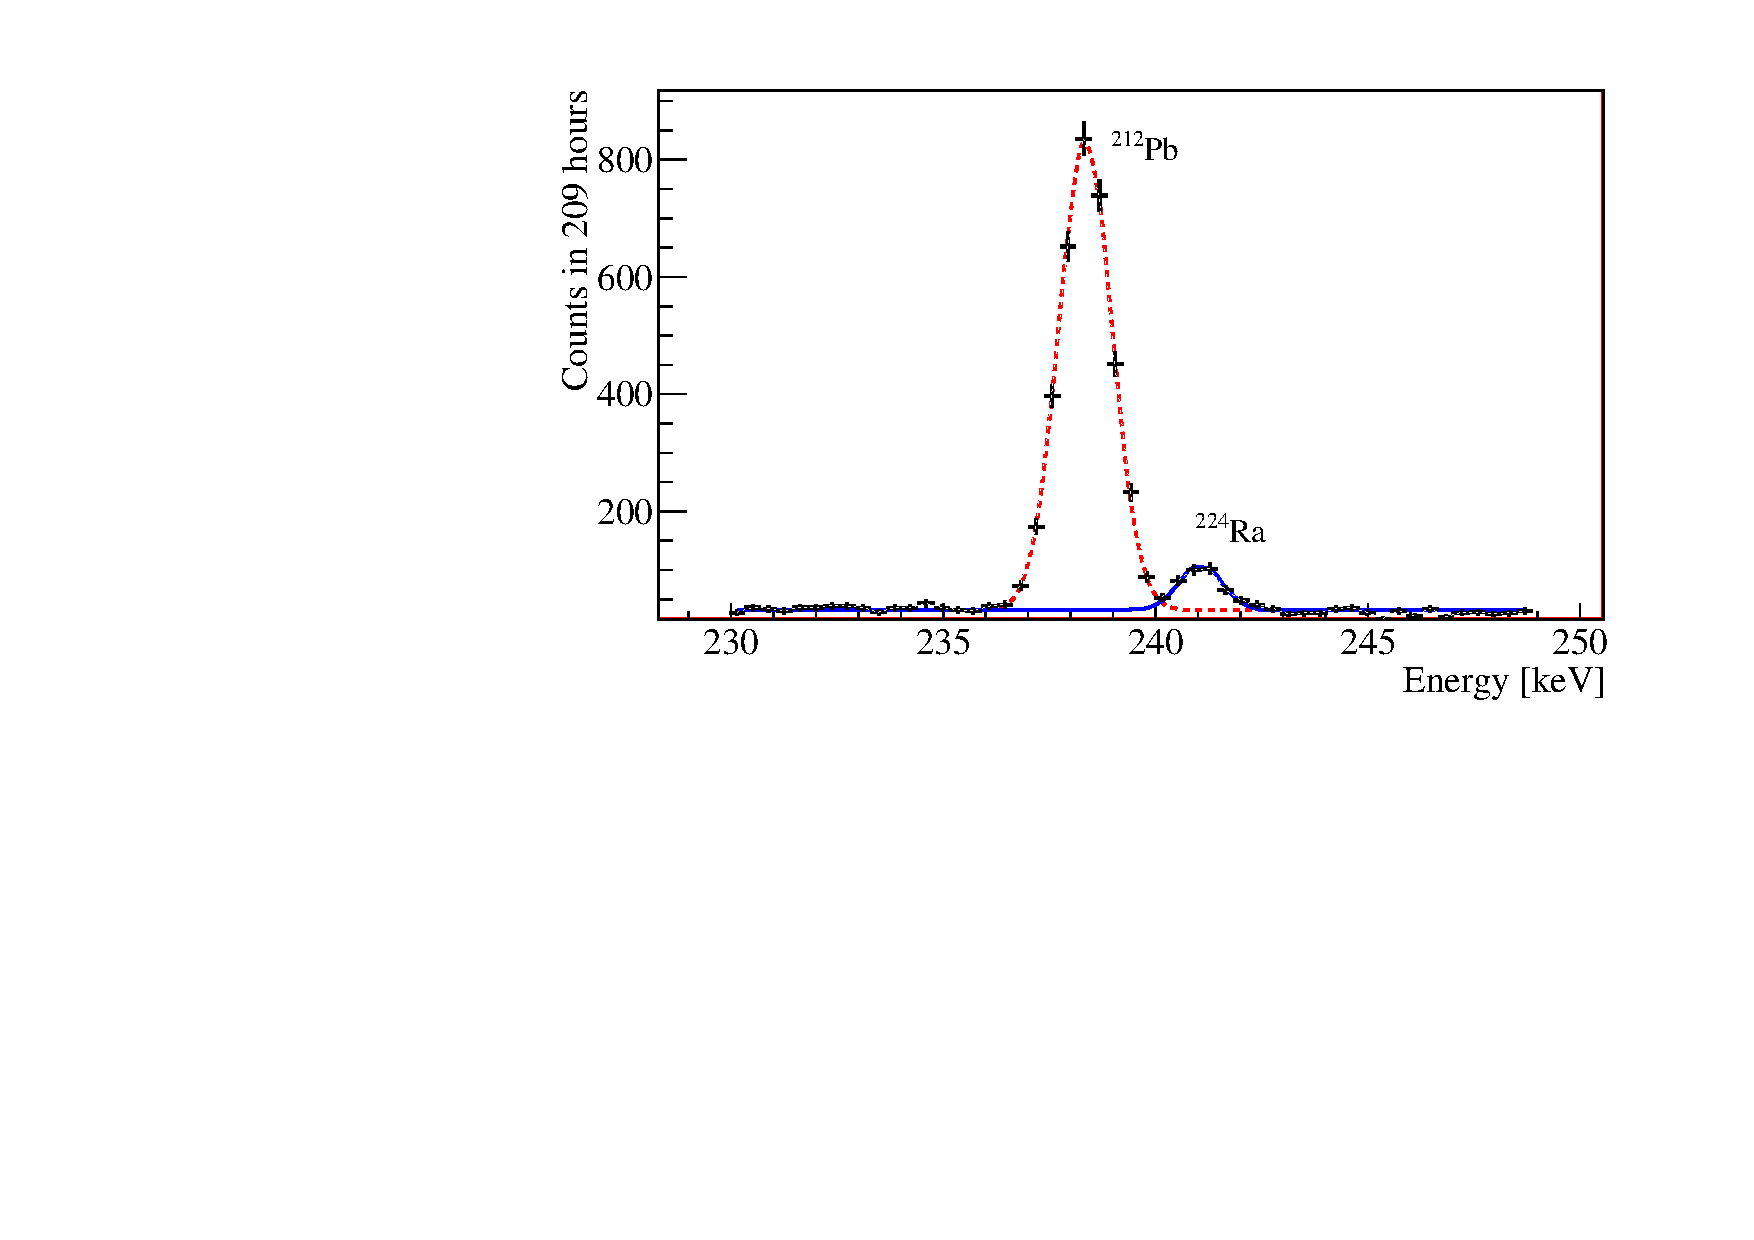
\includegraphics[trim = 15 0 50 20, clip = true,width = 0.8\columnwidth]{figures/rnsource/ge_spectrum}
    \caption{Gamma spectrum taken of the filter 7.2 days after exposure showing the $^{212}$Pb~line at 238.6 keV and the $^{224}$Ra~line at 241.0 keV. The dashed and solid lines are from a fit to the data.}\label{fig:gammaspectrum}
\end{figure}

A week after exposure most of the $^{212}$Pb~has decayed and measurements become sensitive to $^{224}$Ra. A measurement with a livetime of 208 hours yielded a $^{224}$Ra~activity of $(1.0\pm0.3)\1{Bq}$ on the filter at the end of exposure. A second measurement was done forty-two days after exposure, at which point the $^{224}$Ra~deposited on the filter should have decayed to $3\times10^{-4}$ of the initial population. Thus, any measured $^{224}$Ra~activity could be attributed to residual $^{228}$Th. We calculate upper limits (90\% CL) of 2.5 mBq for $^{228}$Th~and 2.4 mBq for $^{224}$Ra~on the filter. These activities convert to emanation rates of $(1.9\pm0.6)\1{atoms/min/kBq}$ $^{224}$Ra~and $<0.4\1{atoms/min/kBq}$ $^{228}$Th.

\section{$^{222}$Rn Emanation Measurement}

Potential traces of $^{226}$Ra or $^{230}$Th in the $^{220}$Rn~source would lead to a non-negligible emanation of the long-lived radon isotope $^{222}$Rn, which must be avoided. We applied ultra-low background proportional counters as described in~\cite{Zuzel:2009} to measure directly the $^{222}$Rn emanation rate of the source. For this purpose the source was connected to a 1 liter stainless steel buffer volume, separated by a valve. The setup was evacuated and the valve was opened such that $^{220}$Rn~and $^{222}$Rn from the source could emanate into the buffer volume. After some days the valve was closed and the buffer volume was separated from the source. When all $^{220}$Rn~had decayed, the $^{222}$Rn was extracted from the buffer volume and filled to a proportional counter in which the alpha decays of $^{222}$Rn and its daughters were counted.

We repeated the measurement three times with a small modification in the the third measurement: instead of emanating into vacuum, we filled 1.5 bar of helium in the buffer volume to check whether there is a difference between radon emanation into gas and into vacuum. It turned out that this is not the case as all three measurements are in good agreement and compatible with zero. The combined result is a $^{222}$Rn emanation rate from the $^{220}$Rn~source of $<55~\mu$Bq.

\section{Si PIN Diode Measurements}
\label{sec:diode}
% radon monitor
A direct measurement of the $^{220}$Rn~source was performed with a custom-developed radon monitor. It consists of a 3-liter vacuum-tight stainless steel vessel containing a 2 cm square windowless Si PIN diode from Hamamatsu. A high voltage of 1.5 kV collects the charged ions resulting from the decays of $^{220}$Rn~onto the surface of the diode, where the $^{216}$Po decay can be detected with an efficiency of about 35\%. The radon detector was calibrated using a $^{226}$Ra solution with a known activity of $(25\pm1)\1{Bq}$ by bubbling nitrogen through the solution, thus obtaining a known activity of $^{222}$Rn.

The $^{220}$Rn~source was placed directly inside the radon monitor, which was filled with air, and $^{220}$Rn~was allowed to reach equilibrium. Assuming the same collection efficiency of $^{222}$Rn and $^{220}$Rn, an emanation of $(1750\pm50)\1{Bq}$ $^{220}$Rn~was determined. After 10~days, the $^{220}$Rn~source was removed from the radon monitor and the vessel evacuated, and all collected ions on the surface of the Si PIN diode were left to decay. Six days after the removal of the source, all $^{220}$Rn~activity would be due to emanated $^{224}$Ra~collected on the surface of the diode. The emanated $^{224}$Ra~activity was calculated to be $(2.1\pm0.7)\1{Bq}$ and the $^{228}$Th~activity as $<50\,\mu\n{Bq}$ at the point when the source was removed, which corresponds to a $^{224}$Ra~emanation rate of $(3.9\pm1.3)\1{atoms/min/kBq}$ and a $^{228}$Th~rate of $<0.008\1{atoms/min/kBq}$.

% absolute emanation
To further determine levels of emanation, the source was placed directly facing a Hamamatsu windowless Si PIN diode that acts as an alpha spectrometer~\cite{Bray:2014}. The source and diode were placed in a small vessel separated by only $8\1{mm}$. The vessel was then evacuated, and the source was left for five days to deposit material onto the surface of the diode. The source was then removed and the atoms deposited onto the diode were left to decay under vacuum. Figure~\ref{fig:pindiodespectrum} shows the total activity in the diode above $1\1{MeV}$ decaying away after the removal of the source.

\begin{figure}[htb]
\centering
    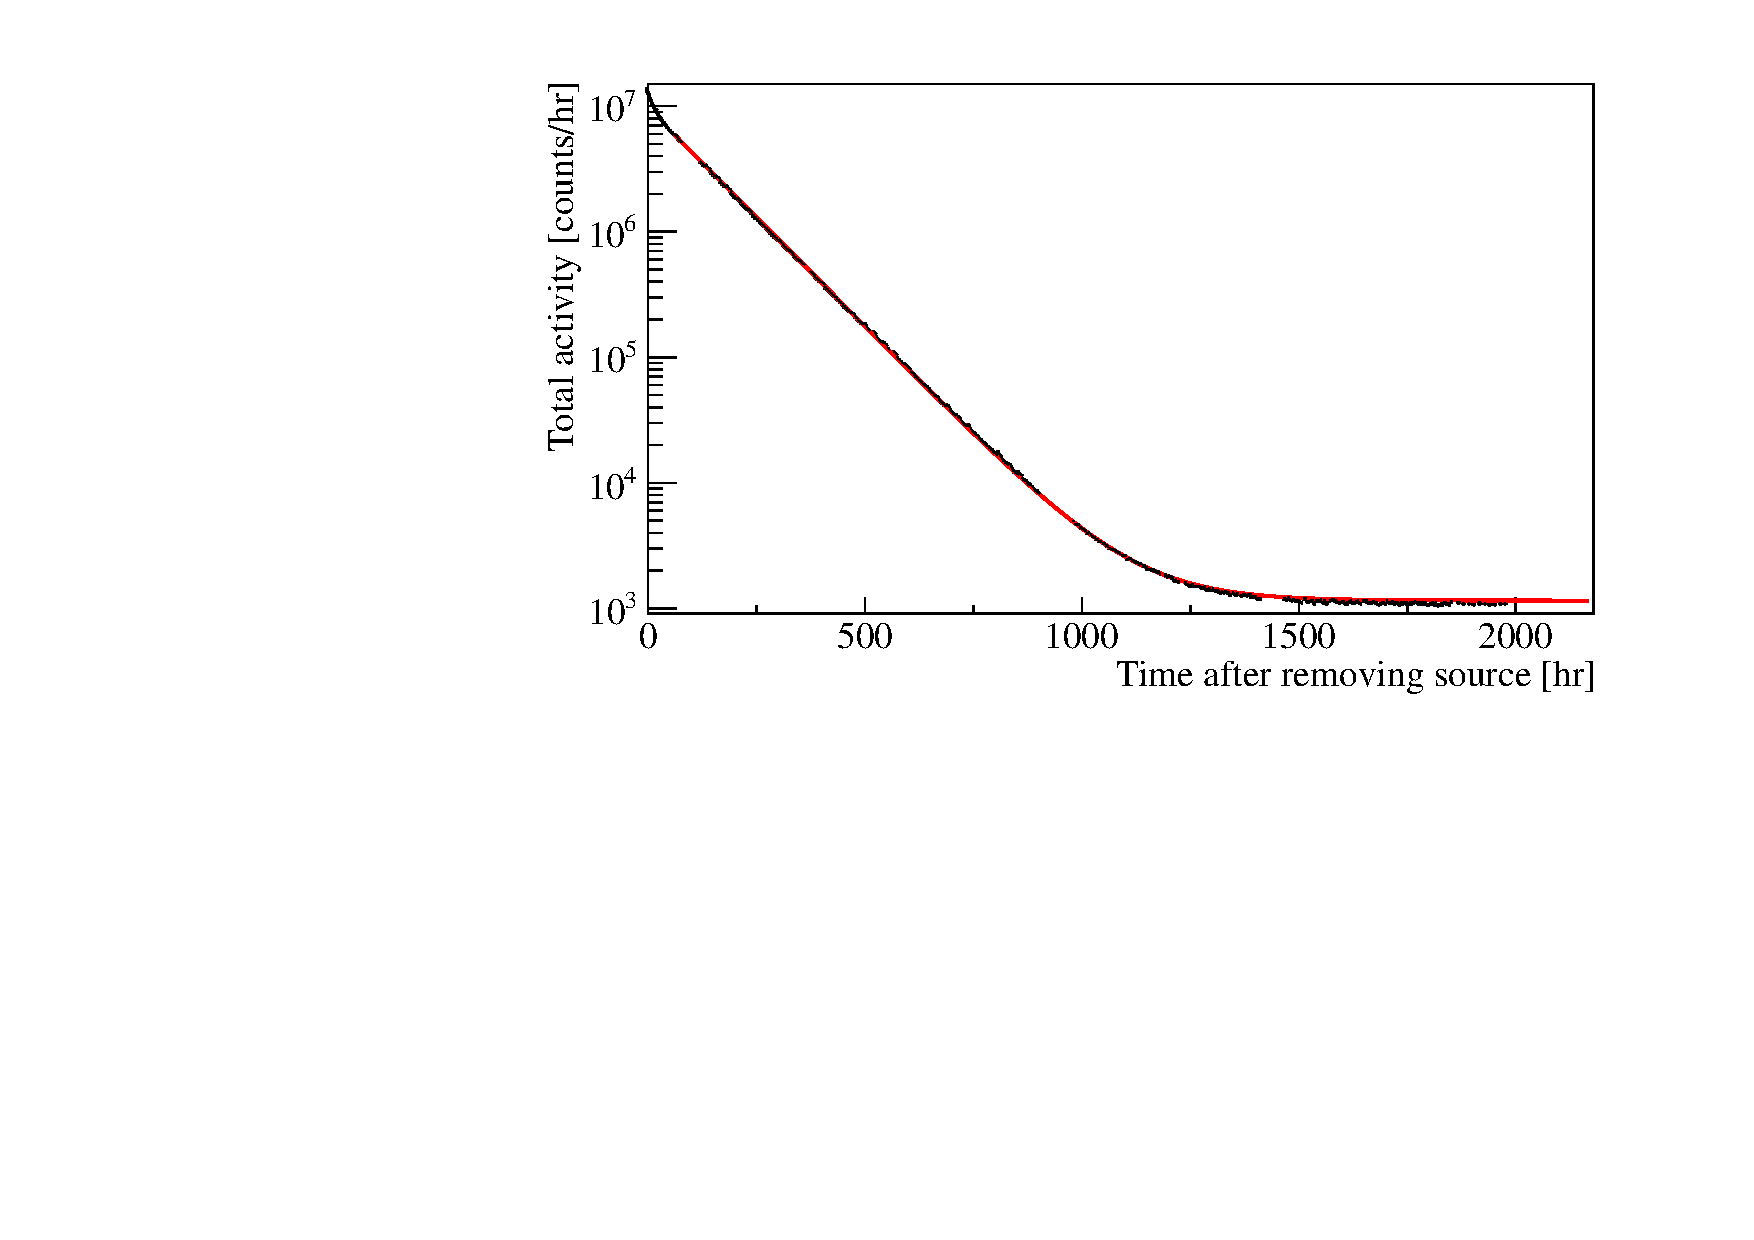
\includegraphics[trim = 5 5 55 20, clip = true,width = 0.8\columnwidth]{figures/rnsource/opensourceactivity}
    \caption{Total activity in the Si PIN diode above 1 MeV. The data points include statistical error bars, barely visible on this scale. The line is the fit of an exponential plus constant baseline.}\label{fig:pindiodespectrum}
\end{figure}

An exponential decay plus a constant baseline is fit to this data, yielding a decay constant in agreement with the accepted half-life of $^{224}$Ra, and a residual background of $(1128\pm3)\1{hr^{-1}}$. Extrapolating the curve backwards and scaling for the fraction of total activity that is $^{224}$Ra, we can calculate the emanation rate of $^{224}$Ra~onto the surface of the diode to be $(924.0\pm0.3)\1{s^{-1}}$. Two months after removing the source, the initial population of $^{224}$Ra~will have decayed away, so the background value inferred from the fit is due to a combination of intrinsic backgrounds (here, measured to be negligible) and released $^{228}$Th. By measuring the activity in the relevant portion of the spectrum, we find a $^{228}$Th~activity of $(0.097\pm0.003)\1{Bq}$, or $(8.4\pm0.3)\times10^6\1{atoms}$. Given the exposure time, this corresponds to a $^{228}$Th~emanation rate of $(18.3\pm0.6)\1{s^{-1}}$ onto the surface of the diode. Simulation with GEANT4 yields a geometric efficiency for deposition of 0.13, which allows us to scale the emanation rates of the source to $(4.5\pm0.2)\1{atoms/s/kBq}$ $^{228}$Th~and $(282.1\pm0.1)\1{atoms/s/kBq}$ $^{224}$Ra.

% Argon flushing measurement
\section{$\gamma$-Spectroscopy of Pipe Contamination}
\label{sec:flush}

A test of radium plate-out was performed by flushing argon from a high-pressure tank through a pressure regulator, the source vessel, and then a copper pipe of $6\1{mm}$ diameter and $50\1{cm}$ length. The argon flow averaged $6\1{slpm}$ though with sizeable fluctuations. After 41~hours of flushing, the copper pipe was cold-welded shut at both ends to seal in any materials deposited on the inner surface, and swiftly transported for measurement using our low-background germanium counters. Several measurements were done over the course of about two months to determine the $\gamma$-activity of the copper pipe. The results of the measurements are given in Table~\ref{tab:flush_meas}.
\begin{table}[htb]
\centering
    \caption{Results of the measured $\gamma$-activity in the cold-welded copper pipe after flushing argon through source and pipe.}
    \label{tab:flush_meas}
    \renewcommand{\arraystretch}{1.2}
    \begin{tabular}{|llccc|}
        \hline\hline
        \multicolumn{2}{|l}{Measurement} & 1 & 2 & 3 \\
        \multicolumn{2}{|l}{Time after exposure} & 10 hours & 7 days & 68 days \\
        \multicolumn{2}{|l}{Livetime} & $76\,733\1{s}$ & $897\,820\1{s}$ & $357\,802\1{s}$ \\ \hline
        \multirow{2}{*}{Activity/Bq}
        & $^{224}$Ra & N/A & $0.25\pm0.03$ & $<0.088$ \\
        & $^{212}$Pb & $13.8\pm0.1$ & $0.215\pm0.005$ & $<0.088$ \\
        \hline\hline
    \end{tabular}
\end{table}

The interpretation of these data is done in a very similar way to that presented in the previous section. The first measurement started approximately 1 half-life of $^{212}$Pb~after exposure, so any amount deposited on the pipe would still be observable. By the time the second measurement was started, a week had passed ($>$15 half-lives), so any initial $^{212}$Pb~would have decayed to a negligible amount, making the measurement sensitive to potential $^{212}$Pb~from the decay of $^{224}$Ra. The interval between exposure and the third measurement is many half-lives of $^{224}$Ra, making the measurement sensitive to potential contamination from the parent $^{228}$Th~in the copper pipe.

\begin{table}[htb]
\centering
    \caption{Calculated values and limits on $^{224}$Ra~and $^{228}$Th~release from deposition in the copper pipe after argon flushing.}
    \label{tab:flush_limits}
    \renewcommand{\arraystretch}{1.2}
    \begin{tabular}{|lcc|}
        \hline\hline
        Isotope & Activity after exposure & Emanation rate \\ \hline
        $^{212}$Pb & $(26.0\pm0.2)\1{Bq}$ & N/A \\
        $^{224}$Ra & $(0.95\pm0.11)\1{Bq}$ & $(1.53\pm0.04)\1{atoms/min/kBq}$ \\
        $^{228}$Th & $<0.093\1{Bq}$ & $<47\1{atoms/min/kBq}$ \\
        \hline\hline
    \end{tabular}
\end{table}

Indeed trace amounts of $^{224}$Ra~appear to have come off the source in this experiment. While the overall activity is very small, it motivates the use of an additional filter just after the source vessel for the calibration of low background detectors.

% Alpha spec at Purdue
\section{Measurements of Filter Efficacy}
\label{sec:rn_filter}

In order to assess the performance of various filters in limiting the release of $^{224}$Ra~from the $^{220}$Rn~source, the source vessel was connected to a xenon gas system. Xenon gas was recirculated through various configurations involving the $^{220}$Rn~source vessel, filters, and a Si PIN diode as an $\alpha$-spectrometer~\cite{Bray:2014}. The source was exposed to the xenon gas stream for a few days, then bypassed, and the decaying activity monitored to measure any released radium. Two filter types were tested for their ability to remove radium from the gas stream. The first filter was a Swagelok F-series 0.5-micron sintered filter, the second was a Swagelok SCF-series ceramic filter.

The source vessel was connected directly to the sintered filter and then to the Si PIN diode with about $1\1{m}$ of 1/4" stainless steel pipe. For the ceramic filter, the extra piping was reduced to 8 cm. Xenon gas at $1\1{barg}$ was recirculated through the gas system at $5\1{slpm}$ for the sintered filter and $10\1{slpm}$ for the ceramic filter. After exposure with the sintered filter in line, the source and filter were bypassed and recirculation continued through the detector vessel for several weeks. After exposure with the ceramic filter, recirculation was stopped and the activity deposited in the detector vessel left to decay. Figure~\ref{fig:bipo} shows the activity of coincident $^{212}$Bi-$^{212}$Po (BiPo) activity in the Si PIN diode for the measurement of the ceramic filter from when the source was opened to three days after the source was closed, when the detector vessel was evacuated.

\begin{figure}[htb]
\centering
    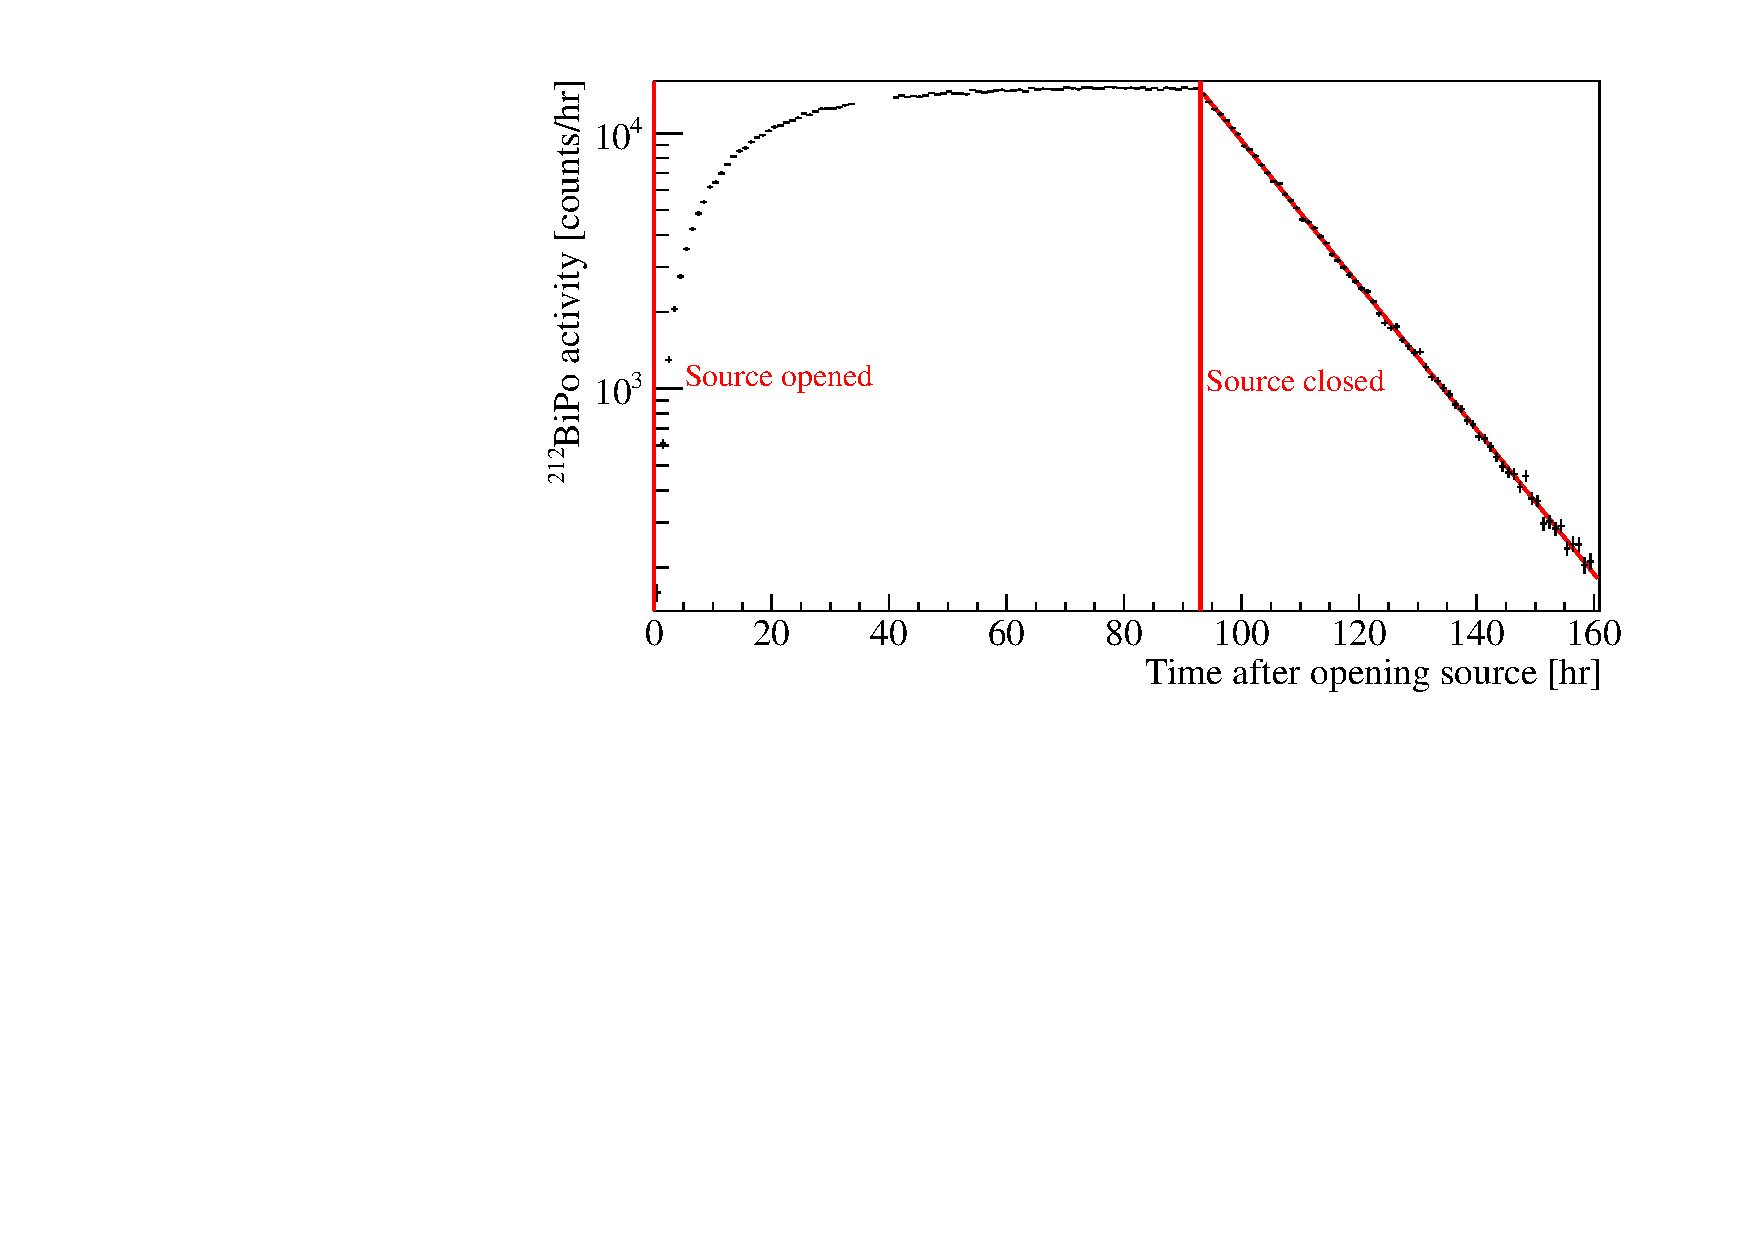
\includegraphics[trim = 5 5 40 15, clip = true,width = 0.8\columnwidth]{figures/rnsource/bipo_activity}
    \caption{Activity of $^{212}$BiPo in the Si PIN diode during and after flushing xenon through the ceramic filter. An exponential was fitted to the decaying part, yielding a half-life of $(10.64\pm0.05)\1{h}$ in excellent agreement with the $^{212}$Pb~half-life of $(10.64\pm0.01)\1{h}$~\cite{Firestone}.}\label{fig:bipo}
\end{figure}

The activity in the Si PIN diode was monitored as the released $^{212}$Pb~decayed to background levels. A summary of the results are given in Table~\ref{tab:filter_limits}. About 14 half-lifes after closing the source the $^{212}$Pb~has almost completely decayed to background levels, at which point any measurement would be sensitive to the release of $^{224}$Ra. The background rate of $^{212}$BiPo events was found prior to these measurements to be $(42\pm7)\1{\mu Bq}$. Figure~\ref{fig:bipo_background} shows the decay for the measurement of the sintered filter, along with a fitted exponential and constant.

\begin{figure}[htb]
\centering
    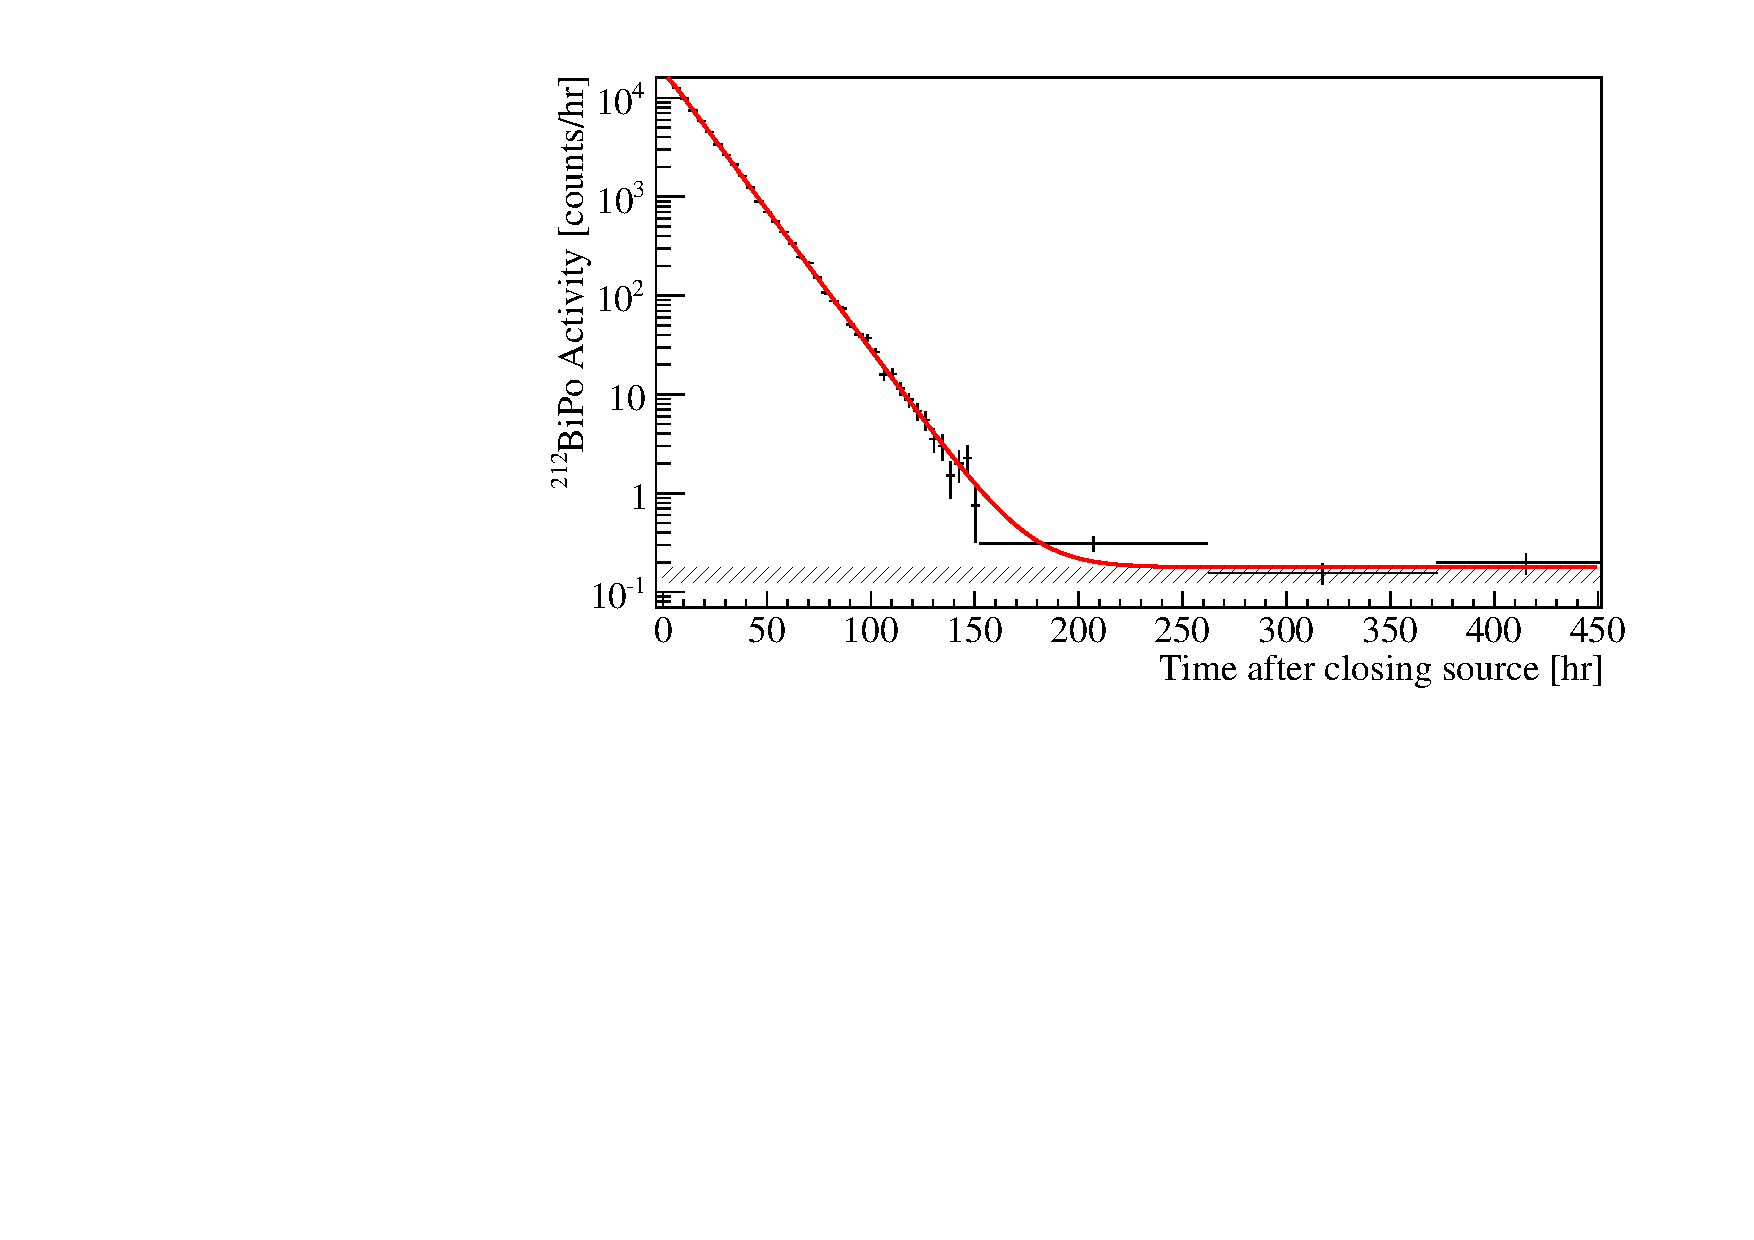
\includegraphics[trim = 10 5 40 15, clip = true,width = 0.8\columnwidth]{figures/rnsource/bipo_background_sintered}
    \caption{Decay to background of $^{212}$BiPo in the Si PIN diode for the measurement of the sintered filter. An exponential and a constant are fitted to the data. The band is the previously measured background of the detector.}\label{fig:bipo_background}
\end{figure}

\begin{table}[htb]
\centering
    \caption{Measurement results for the 0.5 micron sintered and ceramic filters}
    \label{tab:filter_limits}
    \renewcommand{\arraystretch}{1.2}
    \begin{tabular}{|lccc|}
        \hline\hline
        Filter & Exposure & Fitted half-life & Fitted background \\ \hline
        Sintered & $39\1{hr}$ & $(10.64\pm0.11)\1{hr}$ & $(49\pm8)\1{\mu Bq}$\\
        Ceramic & $93\1{hr}$ & $(10.51\pm0.60)\1{hr}$ & $(46\pm8)\1{\mu Bq}$\\
        \hline\hline
    \end{tabular}
\end{table}

Both background values show some increase over the rate measured before this experiment, but in neither case is the increase statistically significant ($1\sigma$ for the sintered filter, $0.43\sigma$ for the ceramic filter). However, we can still (conservatively) attribute these small increases to some released $^{224}$Ra, in which case we can limit the release of $^{224}$Ra~to $<0.65\1{atoms/day/kBq}$ for the sintered filter and $<0.21\1{atoms/day/kBq}$ for the ceramic filter. Thus we see that both filters are highly effective at preventing the release of $^{224}$Ra from the source.

A more direct measurement of filter efficiency was performed by placing two identical 90~micron sintered filters in series in the gas system immediately after the source vessel. After recirculating xenon gas at 6.5~slpm through the source and filters for 100~hours, the two filters were then placed on top of the Si PIN diode to measure any $\alpha$-activity coming off of them that could be attributed to $^{224}$Ra. A total of 4~days of data were taken. The spectra of the two filters is shown in Figure~\ref{fig:twofilters}. While the first filter showed an activity of $(55.4\pm2.1)\1{mBq}$ of $^{224}$Ra, the second filter that was placed immediately downstream of the first only showed an activity of $(1.63\pm0.18)\1{mBq}$ of $^{224}$Ra. Both numbers are corrected for the activity at the time of source closing. Hence, their ratio directly gives the filter efficiency. This value is independent of systematic uncertainties such as the collection efficiency of the Si PIN diode, geometrical effects, etc. We thus find these 90~micron sintered filters to retain $(97.1\pm0.3)$\% of $^{224}$Ra~flushing through them.

\begin{figure}[htb]
\centering
    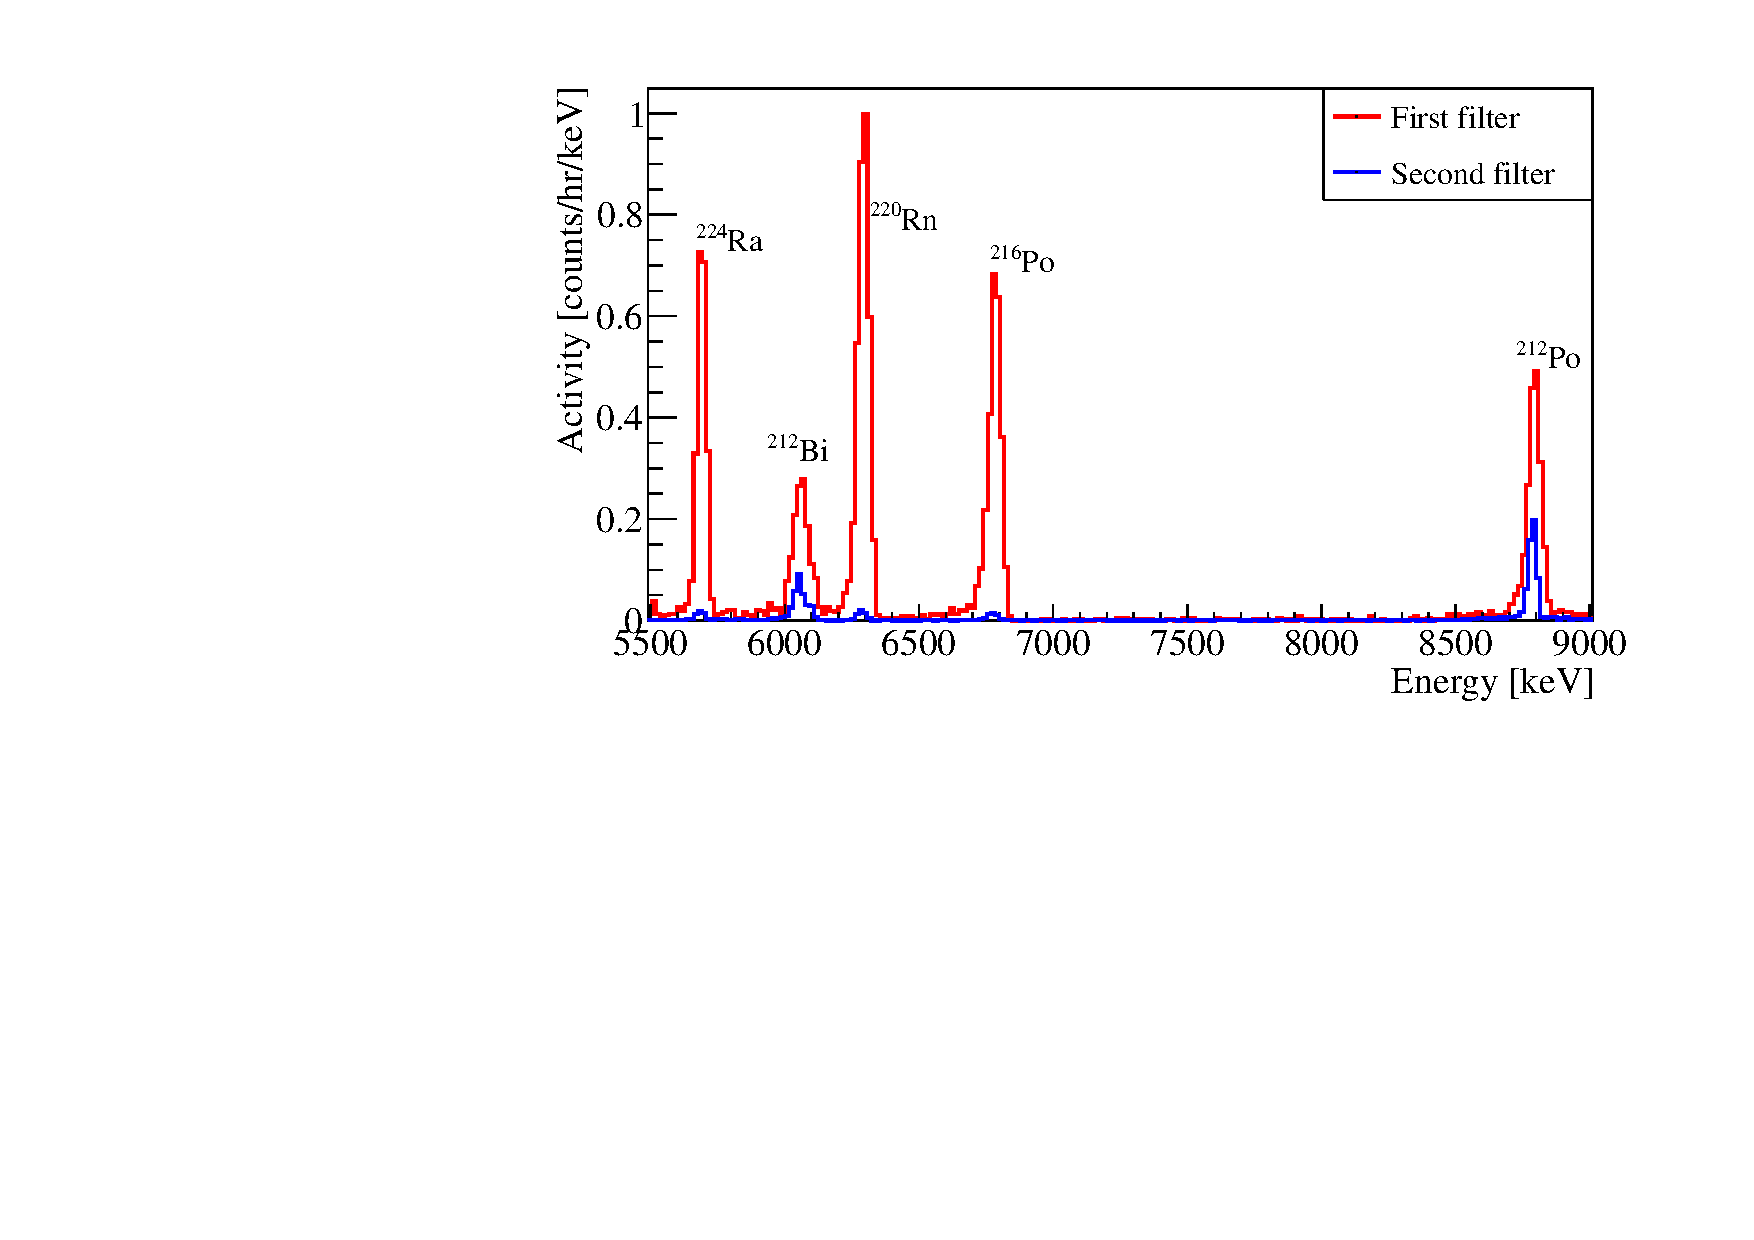
\includegraphics[trim = 5 0 40 20, clip = true,width = 0.8\columnwidth]{figures/rnsource/twofilters}
    \caption{Energy spectrum taken with the Si PIN diode from two sintered filters that were placed in series directly after the source in a xenon gas recirculation system.}\label{fig:twofilters}
\end{figure}

\section{Mixing in a Liquid Xenon Detector}

A liquid/gas xenon TPC was used to test the injection of $^{220}$Rn~into a liquid xenon detector. The detector was designed with a long drift length of 17~cm and a diameter of 80~mm. Each end of the drift chamber is monitored by 7~Hamamatsu R8720 photomultiplier tubes (PMTs). The walls of the TPC are constructed of a single cylinder of PTFE, for use as a UV~light reflector, with field shaping electrodes embedded inside the PTFE walls. The drift and charge amplification fields are applied with transparent meshes at the ends of the TPC to allow for high optical collection. For the measurements presented here, only scintillation light was collected. However, this setup is sufficient to demonstrate that $^{220}$Rn~can be flushed into the detector before decaying so that the subsequent $^{212}$Pb~beta decays can be used as an internal calibrator. The detector was filled with about 3~kg of liquid xenon, which was continuously recirculated at 8.5~slpm through a high-temperature zirconium getter to remove electronegative impurities. The recirculation is done in the gas phase using 1/2" VCR piping with a heat exchanger in the xenon loop~\cite{Giboni:2011wx}, constituting a setup very similar to that of the XENON1T experiment~\cite{Aprile:2017aty}. The $^{220}$Rn~source vessel was connected to the gas recirculation system such that the gas could be flushed past the source or bypass it. Figure \ref{fig:rn_recirc} shows a schematic of the detector, purification loop, and $^{220}$Rn~source. About 5~m of piping connected the $^{220}$Rn~source to the TPC. For comparison, in XENON1T there are about 20~m of piping connecting the source to the TPC, and recirculation is planned for 100~slpm. Taken together, a comparable injection of activity may be expected.

\begin{figure}[htb]
\centering
    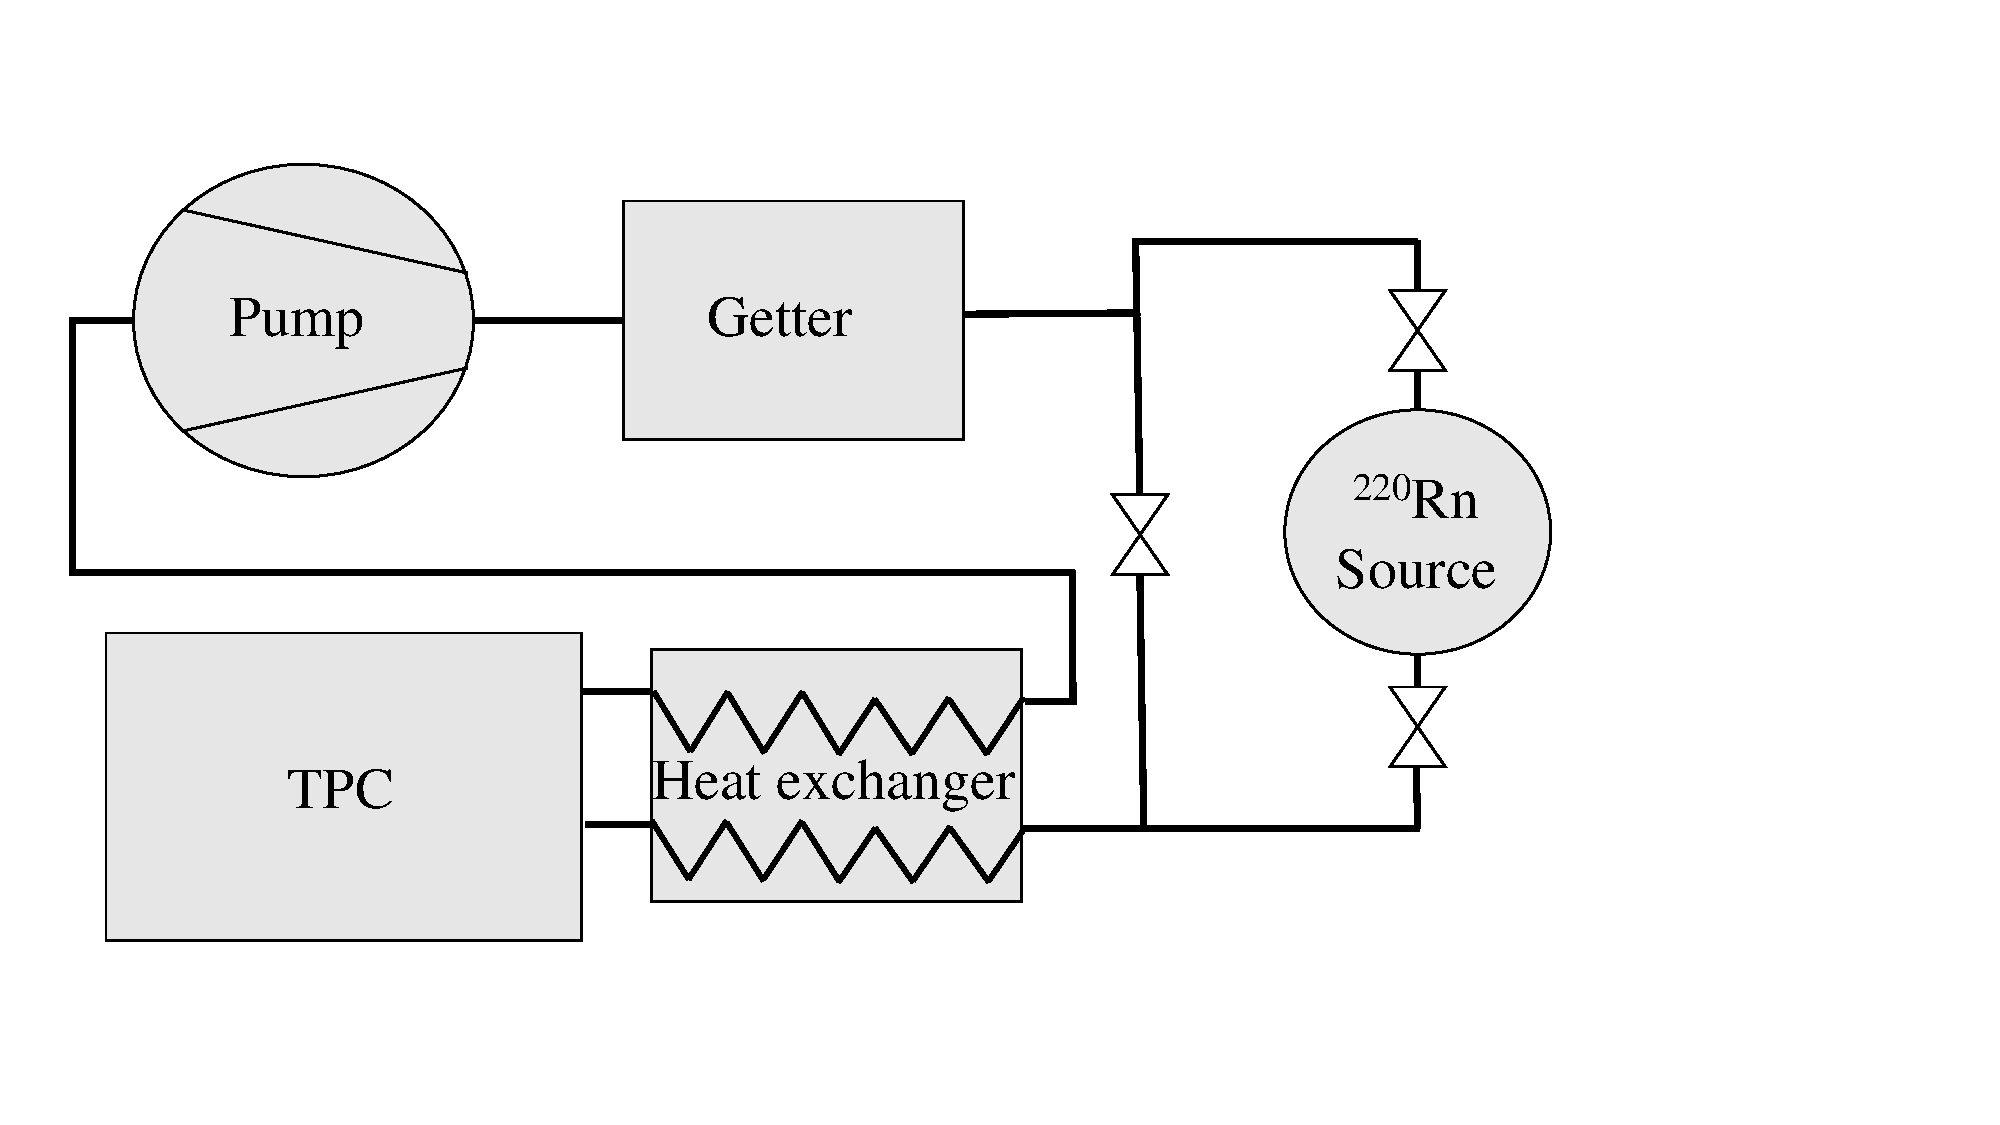
\includegraphics[trim = 0 0 0 0, clip = true,width = 0.8\columnwidth]{figures/rnsource/recirc_schematic}
    \caption{Schematic of the recirculation loop for the liquid xenon detector measurement. The liquid is evaporated in the heat exchanger and is pumped through the purifier, where it can then be flushed past the $^{220}$Rn~source or injected directly back to the detector.}\label{fig:rn_recirc}
\end{figure}

To prove that the $^{220}$Rn~could be mixed into the detector, the source was opened for 22.8 hours, injecting the doped gas. By monitoring the trigger rate of the detector, it was possible to observe the arrival of the dopants into the liquid xenon target. Data were acquired for 2.9~days surrounding this opening to determine the background before opening, and to monitor the decay of the injected $^{212}$Pb~after the source was closed. The resulting trigger rate evolution of high-energy $\alpha$-decays is shown in Figure \ref{fig:rn_rates}. Events were selected by cutting at low energies and enforcing a coincidence requirement on the bottom PMTs. The background trigger rate of 1~Hz quickly rose to a 30~Hz after the source was opened, showing that the activity of the source was entering the liquid xenon target, followed by the growing in of $^{212}$Pb~and its daughters over the next 22~hours. After the source was closed, the trigger rate quickly dropped to 30~Hz, after which it decayed toward the background rate.

\begin{figure}[htb]
\centering
    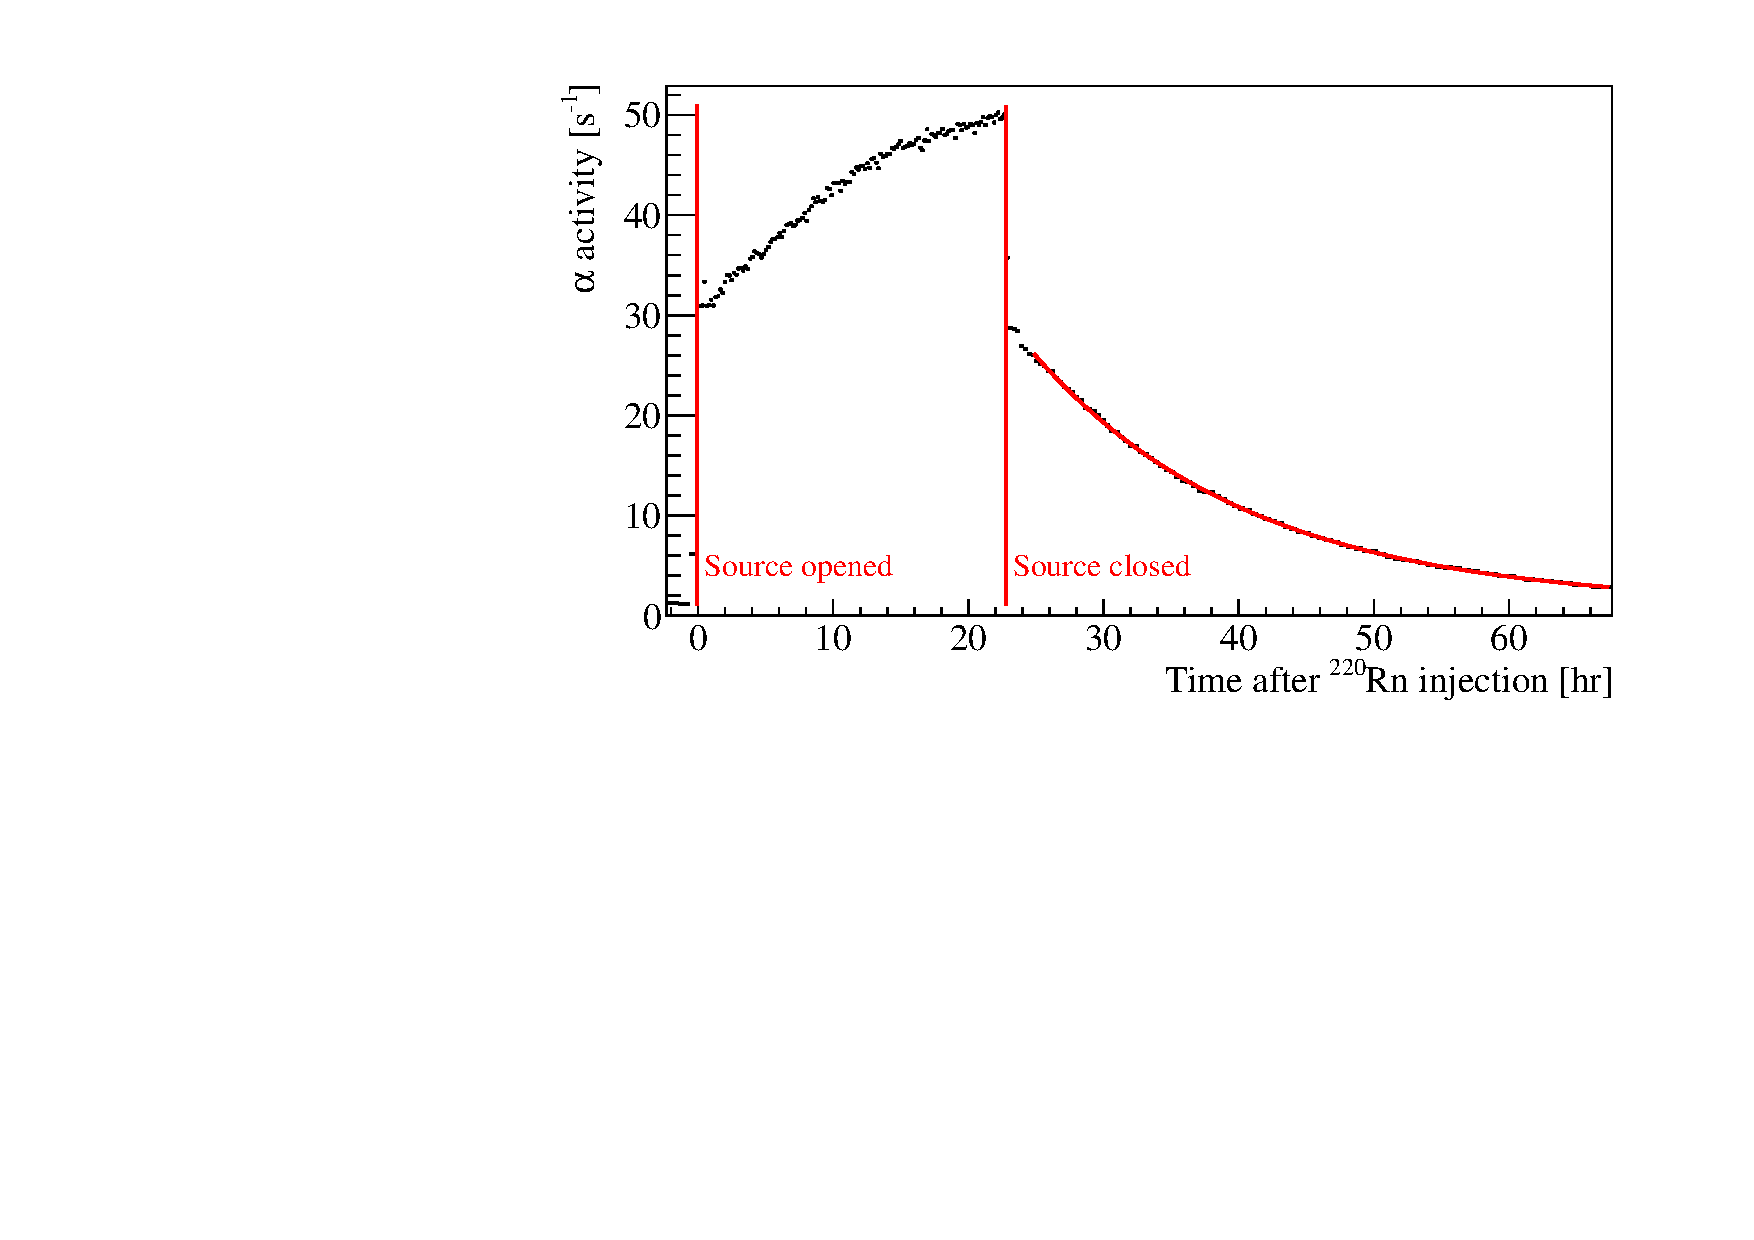
\includegraphics[trim = 0 0 0 0, clip = true,width = 0.8\columnwidth]{figures/rnsource/tpc_rate}
    \caption{Trigger rate of high-energy events in the liquid xenon detector before, during, and after source exposure. After source opening, the $^{212}$Pb~activity grows in, clearly demonstrating the introduction of activity into the target volume. At source closing, the $^{220}$Rn~and $^{216}$Po~alpha activity quickly decays away, leading to a drop in rate. Aterwards, the activity decays more slowly. A fit of an exponential plus constant background onto the decaying edge yields half-life ($11.18\pm0.04$)~hr. This is close to the $^{212}$Pb~half-life, with the difference attributed to dead-time effects. Hence, this data demonstrates the presence of $^{212}$Pb~decays in the TPC.}\label{fig:rn_rates}
\end{figure}

The data acquisition system was not optimized for measuring high rates in a two-phase operation, resulting in a large rate-dependent dead time. This impedes our determination of the actual activity in the target volume, as well as our ability to accurately measure the decay rate following the closing of the source. However, this measurement is clearly sufficient to demonstrate three major features of this source: first, $^{220}$Rn~emanates from the source and can be mixed into a liquid xenon detector. Second, a low activity source is capable of introducing enough activity to be measured even above a high background rate. Third, the decay after the source is closed demonstrates the presence of $^{212}$Pb~in the liquid target, a requirement to use this source for calibration of the low-energy region in a dark matter search.

\section{Interpretation}

\begin{table}[htb]
\centering
    \caption{Summary of all measurements of emanation rates, given in units of atoms/min/kBq.}
    \label{tab:rn_summary}
    \begin{tabular}{|lcc|}
        \hline \hline
        Measurement & $^{228}$Th & $^{224}$Ra \\ \hline
        $\gamma$ measurements of filters, Section~\ref{sec:tuv}  & $<34$ & $<0.66$ \\
        & $<0.4$ & $1.9\pm0.6$ \\
        Pipe contamination, Section~\ref{sec:flush} & $<47$ & $1.53\pm0.04$ \\
        Radon monitor, Section~\ref{sec:diode} & $<0.008$ & $3.9\pm1.3$ \\
        Si PIN diode, Section~\ref{sec:diode} & $270\pm12$ & $16926\pm6$ \\
        Sintered filter, Section~\ref{sec:rn_filter} & N/A & $<4.5\times10^{-4}$ \\
        Ceramic filter, Section~\ref{sec:rn_filter} & N/A & $<1.5\times10^{-4}$ \\
        \hline \hline
    \end{tabular}
\end{table}

Table~\ref{tab:rn_summary} summarizes the various measurements. The two $\gamma$ measurements of filter deposition and the measurement of pipe contamination are methodologically very similar, yet the results are strikingly different. Additionally, the measurement using the Si PIN diode are orders of magnitude different. The apparent inconsistency between the $\gamma$ measurements and pipe contamination can be attributed to deposition of $^{224}$Ra~in the 1/2" piping: in the first two measurements, 18~cm and 8~cm of piping were present respectively in between the source vessel and filter, while the copper pipe was less than 1~cm from the source (leaving just enough space to cold-weld the copper). In the second $\gamma$ measurement, the flow through the source vessel and the filter was laminar, whereas the flow was turbulent for the pipe contamination measurement. Due to its extremely high reactivity, radium will bond readily to pipe walls. This is facilitated by turbulent flow, while in laminar flow, the slow process of radial diffusion will impede the plate-out of $^{224}$Ra. As the second $\gamma$ measurement and the pipe contamination measurement are consistent, we attribute the discrepancy of the first $\gamma$ measurement to the different conditions of the gas flow.

For the measurements of filter efficiency, the limits presented for the ceramic and 0.5~micron sintered filters are very satisfactory, while in the two-filter measurement, the 90~micron sintered filters are only 97\% efficient. However, at the time of this measurement, the source had an activity of around 60~kBq. Hence, the activity seen in the first filter ($55.4\pm2.1\1{mBq}$) shows a drastic reduction in the activity after only a few centimeters of piping. From this, we can conclude that even though the source gives off very large amounts of $^{224}$Ra~and $^{228}$Th~(as shown by the Si PIN diode measurement), only a vanishing percentage makes it out of the source vessel. With these sources being used in a fluid stream, one may thus expect the vast majority of $^{224}$Ra~and $^{228}$Th~to plate out in any connecting piping.

\section{Conclusions}

We have presented a versatile $^{220}$Rn~source for the internal calibration of low-background detectors and demonstrated its suitability. Stray emanation was found to be $<0.008\1{atoms/min/kBq}$ for $^{228}$Th~and $(1.53\pm0.04)\1{atoms/min/kBq}$ for $^{224}$Ra, which can be reduced to $<10^{-3}\1{atoms/min/kBq}$ through the use of an additional filter. We have demonstrated that the $^{220}$Rn~activity can be mixed under realistic conditions in a liquid noble gas detector. The source provides the means by which to calibrate the electronic recoil band in liquid noble element dark matter detectors at low energies, characterize the important radon backgrounds, map fluid dynamics in the liquid target and calibrate those detectors at energies above the Q-value of the $^{136}$Xe double-beta decay. As we have just shown that the emanation of contaminants is negligible, we can deploy this source on experiments such as XENON100~\cite{Aprile:2016pmc} and XENON1T~\cite{Aprile:2017iyp} with confidence.

% convection
% convection, v1.0

\chapter{Convection}~\label{ch:convection}

\paragraph{Abstract} The study of convection in liquid xenon detectors has not at this point been given an exhaustive treatment. While some publications address the topic, no dedicated works on the topic exist. In this chapter we provide some background information about convection in liquid xenon as well as discussion about its measurement.

The analysis of the ${}^{220}$Rn calibration data from XENON100~\cite{Aprile:2016pmc} revealed a buoyancy-driven convection pattern with a considerable $8\1{mm/s}$ fluid speed. A similar analysis from LUX~\cite{Malling:2014} of \Rn~in background data in revealed a pattern with the same features but a higher fluid speed of $3\1{cm/s}$. This was in stark contrast to the lack of convection that was observed in EXO-200~\cite{Albert:2015vma}.

Unless otherwise noted, values for thermodynamic properties of xenon used in this chapter are from NIST~\cite{NIST}.

\section{A review of convection}~\label{sec:convec_review}

The two most common types of convection are natural convection, arising from thermodynamically-driven density gradients, and forced convection, arising from the action of a pump or other device. We will focus here on natural convection, as this dominates over forced convection inside the TPC. The dimensionless quantities commonly associated with natural convection are the Rayleigh and Grashof numbers~\cite{Chandrasekhar:1961,Grashof}, given by

\begin{align}
\n{Ra}_x &= \frac{g\beta\Delta T x^3}{\nu\alpha} = \n{Gr}_x\n{Pr} \\
\n{Gr}_x &= \frac{g\beta\Delta T x^3}{\nu^2}
\label{eq:dimensionless}
\end{align}

Here, $\n{Ra}$ is the Rayleigh number and \n{Gr} the Grashof number, $g$ the earth's gravitational field ($9.8\1{m/s^2}$), $\beta$ the coefficient of thermal expansion ($XX\1{units}$), $\nu$ the kinematic viscosity $XX\1{units}$), $\alpha$ the thermal diffusivity ($XX\1{units}$), $\Delta T$ the temperature difference ($0.3\1{K}$), and $x$ the chracteristic length scale ($1\1{m}$). $\n{Gr}$ relates buoyancy and viscosity, while the Prandtl number $\n{Pr}$~\cite{Prandtl} is the ratio between viscous and thermal diffusion rates and is a function purely of the fluid. For xenon at the temperatures involved here, the value is $XX$.

If we evaluate the Grashof and Rayleigh numbers, we find values of \todo{XX} and \todo{YY} respectively, indicating a laminar boundary layer, and a convection speed of order $\order{XX\1{mm/s}}$.

\section{Convection in XENON1T}~\label{sec:convection}

Given the similarities in the convection patterns between XENON100 and LUX and the differences between how those experiments inject xenon into the active volume, concrete predictions of what to expect in XENON1T are difficult to make. Conceptually, we might expect a similar single-cell pattern, or the increased detector size might allow the formation of two cells. Thus, it is important that any attempt to measure the convection be as agnostic possible, in order to avoid projecting expecations onto the data.

To measure convection we require two decays out of a decay chain so that there is a meaningful correlation between decay vertices. We further impose a number of requirements on these two decays.
\begin{enumerate}
    \item One isotope in the chain must be capable of being injected into the detector and must mix throughout.
    \item The two decays of interest must be easily identifiable and shouldn't confuse position reconstruction in any way.
    \item The livetime of the second decay must be relatively short such that $v_{ave}\tau$ is larger than position reconstruction uncertainties, yet small enough such that within two or three livetimes it's still closer to its parent than any others (to facilitate easy matching).
    \item Any further activity in the decay chain must either decay away quickly or be removable (decay is preferable), unless this measurement is done at the end of the detector's lifetime, in which case this can be relaxed.
\end{enumerate}

Requirememt $(1)$ excludes all decay chains without some gasseous form, or that cannot form some gasseous compount (conceptually similar to $\n{CH}_3\n{T}$ or $\n{UF}_6$). Requirement $(2)$ points towards isotopes that primarily have an $\alpha$ mode, as a high-energy $\gamma$ will scatter multiple times, which makes position reconstruction difficult. Isotopes with $\beta$-decays are difficult to identify due to the lack of defining spectral features. Requirement $(3)$ can be fulfilled by reducing the injected activity, but this then means the measurement requires more time. Furthermore, if the livetime of the second isotope is not short compared to the timescale of convection, this also makes matching difficult, as the effects of curvature of the fluid streamlines will need to be incorporated when the convection map is constructed.

Pairings of radon and polonium are often ideal for this purpose. Both elements tend to decay via $\alpha$ decay and only rarely emit $\gamma$s during the process, which makes clean populations relatively easy to select. Radon, being a noble element, is easy to introduce into the detector and can bypass most purification systems, and, with the exception of \Rn, have no long-lived progeny, fulfilling requirement $(4)$.

\subsection{$^{220}$Rn-$^{216}$Po}

Given how successful the pairing of $^{220}$Rn and $^{216}$Po were for XENON100 for convection measurements, it is a logical place to start for XENON1T. However, as shown in Figure~\ref{fig:rn220}, the only a paucity of the $^{220}$Rn atoms injected into the active volume reach the drift region, with the majority decaying at or below the cathode.

\begin{figure}[htb]
\centering
    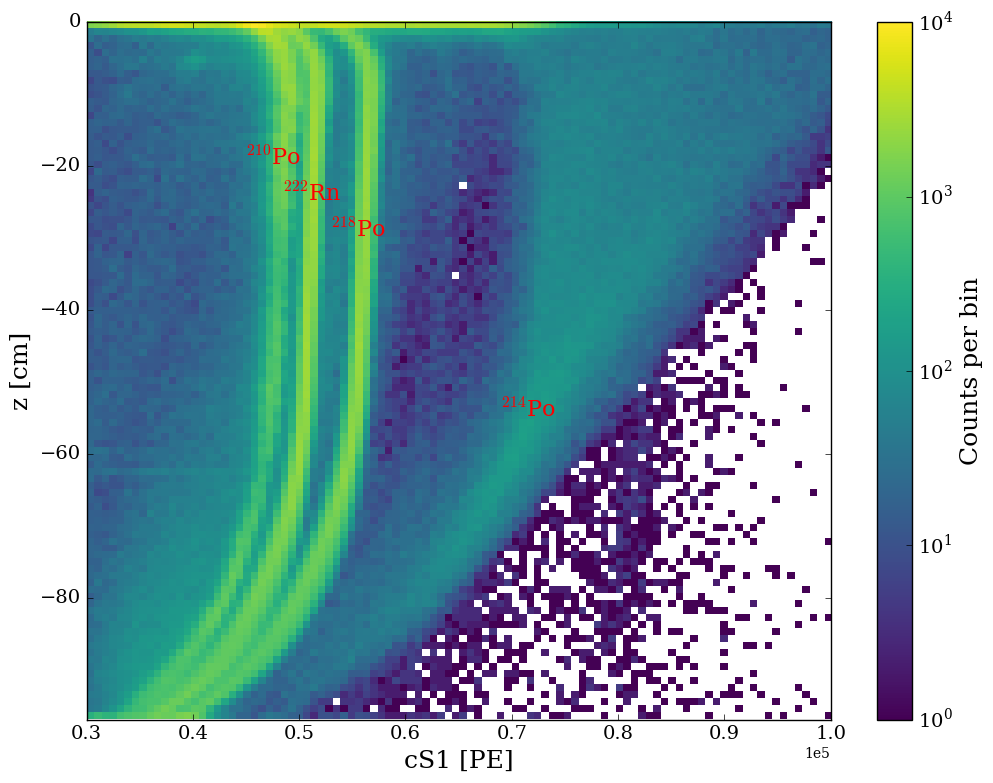
\includegraphics[width=\textwidth]{figures/rnveto/z_cs1}
    \caption{\todo{PLACEHOLDER IMAGE} A plot of {\textit s1\_area\_fraction\_top} (the fraction of the S1 seen by the top PMT array, an excellent proxy for the $z$ coordinate) versus {\textit s1} for the alpha ROI using $^{220}$Rn calibration data. The majority of events are in the very bottom of the detector at or below the cathode, with only a few reaching the drift region where convection can be measured.}\label{fig:rn220}
\end{figure}

\subsection{$^{222}$Rn-$^{218}$Po}

Another available option to match \Po~decays to their parent \Rn~decays. This is a far less trivial endeavour, as the $3.1\1{min}$ half-life of \Po~is quite lengthy, so even at a very modest $1\1{mm/s}$ convection speed, half of all polonium atoms will move 10s of cm away from their parents. Also, the \Rn~background is both boon and bane. As it is mixed uniformly, this provides potential matched pairs in the entire active volume, however no \Rn~or \Po~decays will happen very far from another \Rn~or \Po, which increases the probability of forming incorrect matches.

The \Rn~background rate is $14\1{\mu Bq/kg}$, for a total activity in the active volume of $28\1{mBq}$. The population of \Rn~necessary to provide this activity is easily found via $R = \frac{\dd N}{\dd t} = -\lambda N$, where $R$ is the rate, $\lambda = \ln 2/t_{1/2}$ the decay constant, and $N$ the number of atoms. Thus, we find the \Rn~population size is about $13\,300\1{atoms}$. These will mix uniformly throughout the detector, giving an average distance between \Rn~atoms to be $3.9\1{cm}$. We apply the same calculations for \Po~and find an average population of $7.5\1{atoms}$. The small population of \Po~means the normal Poissonian fluctuations will have a more significant impact than on \Rn.

\subsubsection{Decay identification}

Selection of \Rn~and \Po~is very straightforward. A plot of the reconstructed $z$-coordinate versus cS1 is shown in Figure~\ref{fig:z_cs1} for alpha decays.

\begin{figure}[htb]
\centering
    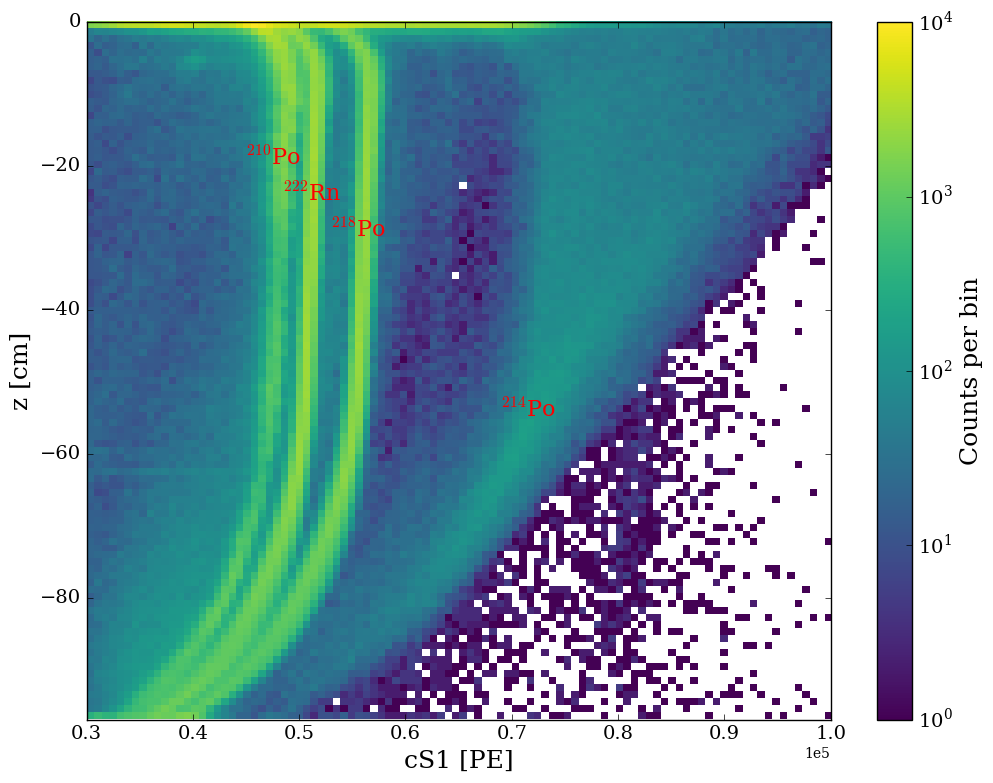
\includegraphics[width=\textwidth]{figures/rnveto/z_cs1}
    \caption{Reconstructed $z$ position versus corrected scintillation light for the alpha ROI. Note the breakdown of the correction factor towards the top and bottom as PMT saturation becomes significant. Four pouplations are evident in the bulk: $^{210}$Po, \Rn, \Po, and $^{214}$Po. The $^{214}$Po is often misreconstructed due to the topology of \BiPo~events deep in the detector, which smears out its population.}\label{fig:z_cs1}
\end{figure}

The $^{210}$Po population exists nearly exclusively on the PTFE reflectors that form the wall of the TPC; a radial cut of even one or two cm significantly reduces its size. The $^{214}$Po band shows up much more clearly if one considers {\it s1\_area\_fraction\_top} rather than $z$, as the short half-life of $^{214}$Po causes some confusion for event reconstruction of the $^{214}$Bi-$^{214}$Po events. The larger S1 from the $^{214}$Po is often paired with the larger S2 from the $^{214}$Bi, resulting in a drift-time that is shorter than the actual value by the livetime of the $^{214}$Po atom.

As we are primarily interested in the center two populations, we can readily select them in the bulk by drawing a few curves on Figure~\ref{fig:z_cs1}, although this tends to break down close to the cathode or liquid surface as the populations smear together. Alternately, machine learning algorithms can exploit separations in multiple parameter spaces simultaneously, providing some additional selection power in these edge regions (see Appendix~\ref{app:ml}).

\subsubsection{Decay matching}

Armed with reasonably clean populations of \Rn~and \Po, the work of decay matching can begin. To do this in as agnostic a fashion as possible, we begin by plotting the temporal and spatial separations of all \Rn~and all \Po~pairs in Figure~\ref{fig:dsdt}. As we can see, most of this parameter space is dominated by random, incorrect pairings. Within a minute after the \Rn~decay, its \Po~daughter merges with the bulk population and cannot be identified with an agnostic approach.

\begin{figure}[htb]
\centering
    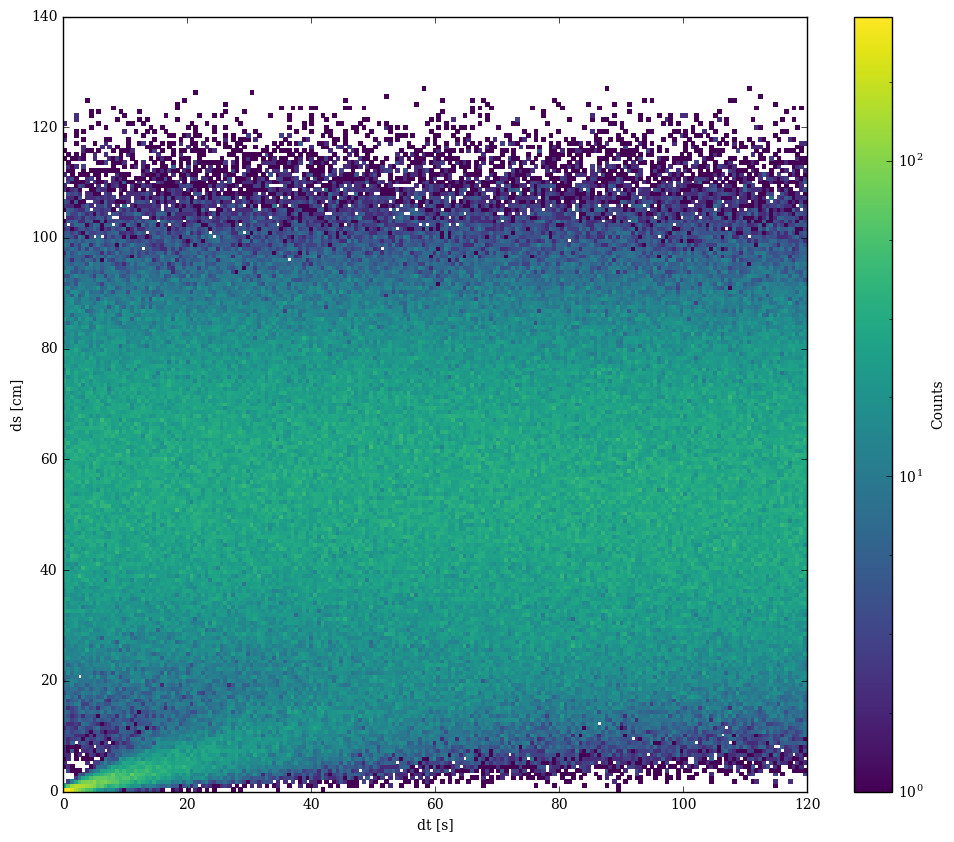
\includegraphics[width=\textwidth]{figures/rnveto/dsdt}
    \caption{Spatial and temporal separations of \Rn~and \Po~events. The ``signal'' population of decay pairs begins at the origin and quickly merges with the ``background'' band of random pairs. Thus, an agnostic approach becomes difficult at times longer than about 45 seconds or distances further than about $15\1{cm}$.}\label{fig:dsdt}
\end{figure}

If we restrict ourselves to potential matches within 30 seconds, this reduces a significant amount of background. Even though this only gives $1-\exp \lambda_{\mathrm{Po}}t = 10\%$ of all possible decays, one day's worth of background data contains some $2500$ total \Rn~decays, or about $7500$ matched decays per month. Evenly spread over the active region, this is one match every $5\1{cm}$, which is sufficient to do a preliminary mapping of convection.

\subsection{Convection map}

By building a three-dimensional map of the displacement of each matched pair we see the shape of the pattern is, as in XENON100 and LUX, a single cell, with much lower speeds of around $3\1{mm/s}$. Figure~\ref{fig:convec} is a projection approximately along the axis of angular momentum.

\begin{figure}[htb]
\centering
    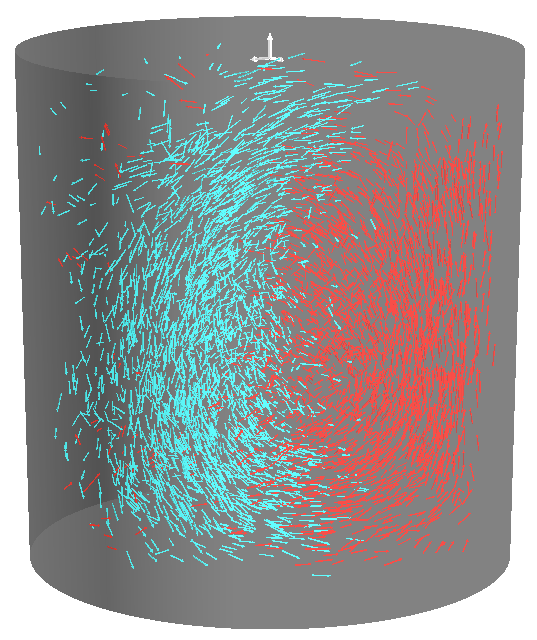
\includegraphics[width=\textwidth]{figures/rnveto/convection_full}
    \caption{The measured convection field in XENON1T. Blue arrows indicates upward movcement; red, downward. A single cell pattern, as was observed in XENON100 and LUX, is clearly seen. Typical speeds are $3\1{mm/s}$.}\label{fig:convec}
\end{figure}

We also see some interesting behavior in the corners. The lack of pairs in these regions indicate a few things. It is unlikely that there is no \Rn~there, but it is entirely possible that our event selection requirements perform very poorly here. This also might be interpreted as hints of counter-current eddies forming in the corners of the detector.

Once a preliminary map is made, this can be used to distinguish correct pairings of \Rn~and \Po~from random matches. The vector connecting two decay verticies should be approximately aligned with the convection cell for correct matches and have a random direction for the incorrect matches. Additionally, because there is at most one \Po~for each \Rn, once a given \Rn~or \Po~has been matched, all other potential matches involving either atom can be removed from consideration.

The combination of these effects allows for an interative process where the matches with the smallest separations (having the best signal to background ratio) are chosen, and any other matches involving these are removed, which reduces the background to all further matches. This can be done again with matches with slightly larger separations.

\section{Simulation}

As the manner of xenon injection in XENON100, LUX, and XENON1T are all different yet all three have the same convection pattern, we can conclude that recirculation does not have a significant impact on convection. Thus, a computational fluid dynamics (CFD) simulation can have some predictive power between experiments, as long as the thermodynamic boundary conditions are correctly modeled. Additionally, a convection field from simulation can probably reveal more about the underlying detector operation than measurements from data.

A variety of different software packages, commercial and otherwise, are available to do this kind of simulation. ANSYS Fluent~\cite{fluent} was used for this work on advice from professor Carlo Scalo of Purdue engineering, also because it is available on the Purdue computing clusters.

A simplified model of the active volume was used to build the simulation mesh, and thermodynamic data from NIST~\cite{NIST} was used at the operating conditions of the detector. The Boussinesq approximation~\cite{Boussinesq:1897} was used to model the density. As we expect laminar, buoyancy-driven flows, the approximation is valid. A representative result is shown in Figure~\ref{fig:cfd_sample}.

\begin{figure}[htb]
\centering
    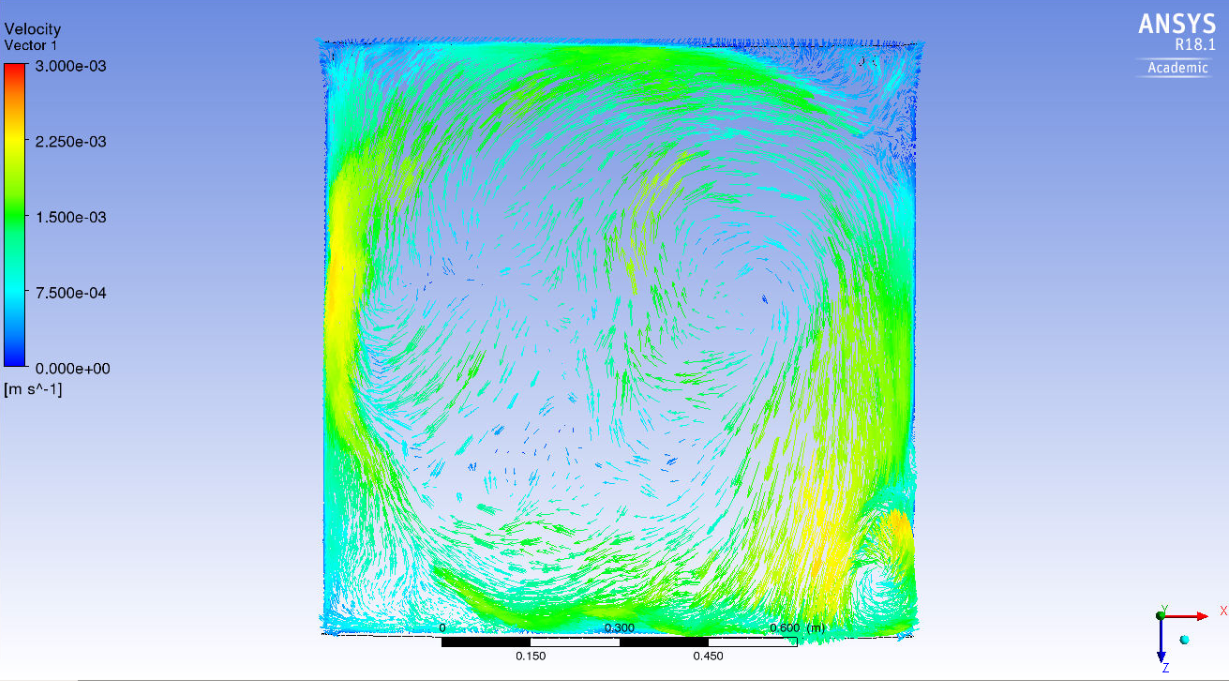
\includegraphics[width=\textwidth]{figures/rnveto/convection_sim}
    \caption{\todo{PLACEHOLDER IMAGE} Simulated convection pattern for XENON1T. A single cell is evident with speeds of a few mm/s. A simple temperature gradient is sufficient to drive this system, though the mechanisms that determine the direction of angular momentum is not yet understood. Counter-currents can be seen in the corners.}\label{fig:cfd_sample}
\end{figure}

Simulations for both steady-state and transient results were performed. The results agree qualitatively with each other, although vortex shedding from counter-currents in the corners are routinely observed.

\section{Comparison between simulation and data}

The simulation results agree qualitatively with the data. A simple temperature gradient is sufficient to establish and drive a single-cell convection pattern, although the symmetry-breaking mechanism that determines the orientation of the pattern is not yet understood. No correlation has been found between the layout of pipes to and from cryogenics and purification and the direction of cell angular momentum.



% radon veto
% chapter six: radon veto

\chapter{The radon veto}~\label{ch:rnveto}

If it is possible to follow atoms of \Po~around the detector, the next step is to follow atoms further down the decay chain. If \Pb~atoms can be followed and their decays identified, these events can be removed from the analysis. As \Pb~is the dominant background source in the dark matter region of interest~\cite{Aprile:2015uzo}, this has the possibility to significantly boost the sensitivity of the experiment at a marginal cost in exposure. We exploit the fact that because \Pb~is part of a larger decay chain, the times and positions of its decays have physical significance to the atoms surrounding it.

We will begin with a brief review of the relevant portion of the decay chain of primordial uranium, as shown in Figure~\ref{fig:useries}. \Pb~decays to the ground state of $^{214}$Bi with a branching ratio of $11.0\%$, and a fraction of these decays lie in the dark matter signal region of interest. This is the primary cause of background in this energy range~\cite{Aprile:2015uzo}.

\begin{figure}[htb]
    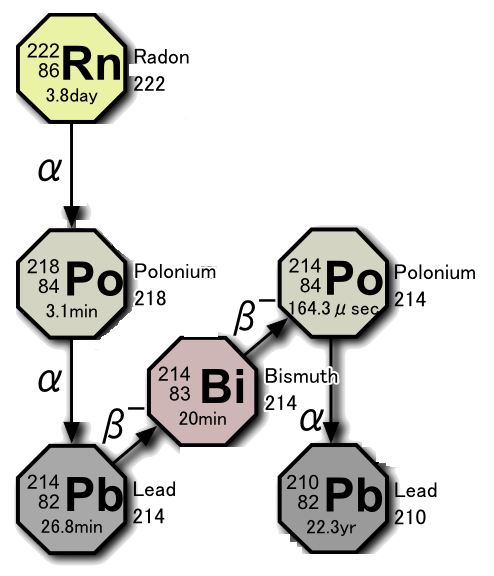
\includegraphics[width=\textwidth]{figures/rnveto/uranium_series}
    \caption{\todo{PLACEHOLDER IMAGE} A section of the decay chain of primordial ${}^{238}$U. Atoms of \Rn~emanate out of impurities in the metals used in detector construction and mix throughout the xenon volume. Low-energy decays of \Pb~that decay directly to the ground state of $^{214}$Bi are the leading cause of background in the dark matter ROI.}\label{fig:useries}
\end{figure}

\section{Technique overview}

While there is nothing about a \Pb~event that is easily identifiable, its parent isotopes (\Rn, \Po) and daughter (\BiPo) can be identified with relative ease using alpha spectroscopy or the BiPo timing structure~\cite{Aprile:2017fhu}. This allows us to bookend the \Pb~event with events that are more easily identified. With this information, an algorithm resembling one for track reconstruction can be employed to improve the confidence with which \Pb~events are tagged by identifying the decays of the parents and daughtber and looking for the convection streamlines that connect them. The \Pb~decay must happen somewhere on the streamline between the \Po~and \BiPo~decays. A stylized representation of this is shown in Figure~\ref{fig:rnveto_schematic} where displacement due to convection is normalized out.

\begin{figure}[htb]
    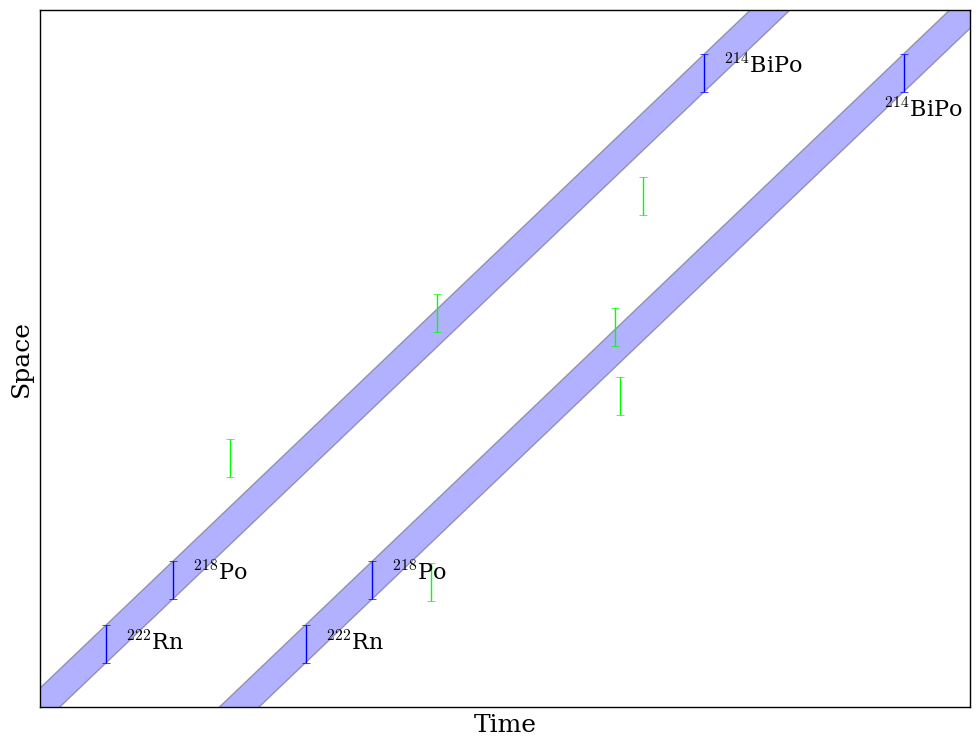
\includegraphics[width=\textwidth]{figures/rnveto/schematic}
    \caption{A simple schematic of how the radon veto works. Low-energy events (in green) due to \Pb~can be identified because they occur on streamlines (shaded regions) connecting \Rn, \Po, and \BiPo~events (in blue), while low-energy events due to other background sources occur at random.}\label{fig:rnveto_schematic}
\end{figure}

\section{Convection-agnostic approach}

To demonstrate a proof of this concept, we employ a convection-agnostic approach. In this method, a sphere is placed around every \Po~or \BiPo~event. Regardless of the size of the sphere or how long one watches it, some fraction of \Pb~decays will occur within it. The size of the sphere can be connected to the length of observation time by the average speed of convection, and the observation time can be chosen by a simple optimization to maximize the potential background reduction while minimizing the overall exposure cost.

The principle background to this Big Sphere method is that of false positives from random coincidence. This can be very easily quantified by placing spheres at random locations and random times within the detector, monitoring the sphere for the specified duration, and counting the number of times a low-energy event is observed. This can then be repeated using locations and timestamps of \Po~or \BiPo~events rather than at random. This allows for the clear quantization of the significant of the result. This was appllied to science run 0, with results shown in Figure~\ref{fig:bs_sr0}.

\begin{figure}[htb]
    \includegraphics[width=\textwidth]{figures/rnveto/BigSphere}
    \caption{\todo{PLACEHOLDER IMAGE} The background estimation for the convection-agnostic Big Sphere method for science run 0. The background from false positives is well-modeled with a binomial distribution. The number of events found by searching near \Po~and \BiPo~is \todo{XX}. This has a p-value of \todo{YY}, indicating a significant result.}\label{fig:bs_sr0}
\end{figure}

\section{Cloud approach}

The Big Sphere method has a number of limitations. Looking in all directions rather than just along the convection streamlines wastes a large amount of exposure, and in cases where multiple low-energy events are observed within the sphere it is impossible to know which is due to the \Pb. At most one can be due to \Pb, yet without additional information it is impossible to determine which. This additional information is from convection. If an event is on known fluid streamlines originating from the \Po~decay vertex or converging to the \BiPo~vertex, it is more likely to be \Pb~than if it occurred far from those streamlines or on otherwise impossible paths.

The computational cost of following these streamlines is non-trivial. It involves a numerical integration of a vector field, and doing this multiple times. Each \Rn~atom can potentially produce a low-energy \Pb~event, so streamlines around every \Rn~must be followed. At a decay rate of $\approx 2500\1{day^{-1}}$, a tonne-year of exposure will contain nearly $500\,000$ total \Rn~events. Streamlines from each of these events must be integrated for (on average) one hour, at sufficiently small timesteps to minimize integration errors.

\section{Diffusion-limited case}

The dominant uncertainties to the radon veto stem from the lack of complete knowledge of the convection pattern. However, we can explore the possibilities of the technique should a perfect understanding of convection be obtained. In this limit, the dominant uncertainties are from position reconstruction and diffusion.

\subsection{Diffusion effects}

When an event happens, we reconstruct its interaction vertex with a uncertainty of $5\1{mm}$ in r and $1\1{mm}$ in z. For reasons we will discuss shortly, we will take 2 sigma and double these. Thus, we assume this event happens somewhere in a cylinder of volume $\approx 630\1{mm^3}$. This cell will follow the convection lines through the volume, growing in time due to diffusion. We'll need a few values here:
\begin{itemize}
    \item $r_0 = 10\1{mm}$
    \item $h_0 = 2\1{mm}$
    \item Cell volume: $V(t=0) = \pi r_0^2h_0 = 630\1{mm^3}$
    \item Diffusion constant: $D = \frac{k_BT}{6\pi\eta r} = 1.7\times10^{-3}\1{mm^2/s}$
\end{itemize}

We find the diffusion constant via the Stokes-Einstein relation for diffusion of a spherical particle through a fluid at low Reynolds number~\cite{Sutherland:1905,Einstein:1905,Smoluchowski:1906}. $\eta$ is the viscosity ($0.5\1{mPa s}$~\cite{Legros:1965}) and $r$ is the radius of the particle in question (taken as $0.15\1{nm}$). The displacement of the atom from its initial location will be roughly given by $\Delta s = \sqrt{\pi Dt}$, and the increase in volume can be found by adding $\sqrt{\pi Dt}$ to both r and z. Thus

\begin{equation}
V(t) = \pi(r_0 + \sqrt{\pi Dt})^2(h_0 + \sqrt{\pi Dt})
\end{equation}

Starting from a decay of \Po, in one half-life of its daughtber ($\sim$30 min) the cell volume will increase by $2.1\1{cm^3}$ to $2.75\1{cm^3}$. If we see an ER event in this volume in the energy range we would expect from a \Pb~decay, we can cut this event (and stop following that cell as it is no longer a potential background event).

\subsection{Total vetoed volume}

The next value to calculate is what fraction of the active region we can follow. For that we need to calculate how many atoms we need to follow at any one time. As calculated above, we find that on average the detector will contain these populations:
\begin{itemize}
    \item $N_{Rn} = 13\,300$
    \item $N_{Po} = 7.5$
    \item $N_{Pb} = 66$
    \item $N_{Bi} = 48$
\end{itemize}

Atoms further down the decay chain will have slightbly reduced populations due to plateout and cathode cleaning, but these values are upper limits. The probability that we must still follow the atom in that volume $P(t) = \exp -\lambda t$ (if the atom decays, we no longer need to follow it), and the expression for the cell volume is given above.

If we wish to reduce the contribution of \Pb~to the low-energy background to the point where it becomes equivalent or subdominant to the other sources of ER background, this requires that we veto about 90\% of all low-energy lead events. This means we have to follow a cell for 3 or 4 half-lives, and for this reason we took 2 sigma of the position uncertainty (giving us 95\% of the atoms). The results change very little if we follow the atom around for an infinite number of half-lives. So, for the math we are about to do, we will integrate over all time, not just the few half-lives we need, and use the resulting closed-form expressions.

To find the average cell volume we integrate the volume $V(t)$ with the probability density $P(t) = \lambda \exp -\lambda t$ to get

\begin{equation}
\left< V \right> = \int_0^{\infty} \dd t\,V(t) P(t) = \int_0^{\infty} \dd t\,\pi(r_0 + \sqrt{\pi Dt})^2(h_0 + \sqrt{\pi Dt})\lambda\exp -\lambda t
\end{equation}

The result is

\begin{equation}
\left< V \right> = V_0 + a\sqrt{\chi} + b\chi + c\chi^{3/2}
\end{equation}

where
\begin{itemize}
    \item $\chi = \frac{D}{\lambda}$ (units of $\n{mm^2}$)
    \item $a = \frac{\pi^{2}}{2} (r_o^2+2 r_0 h_0) = 690\1{mm^2}$
    \item $b = \pi^2 (2r_0 + h_0) = 220\1{mm}$
    \item$c = \frac{3}{4} \pi^{3}$
\end{itemize}

For \Pb, $\chi = 4\1{mm^2}$, so $\Delta V = 2.5\1{cm^3}$ or the total volume we must follow per atom is $V_0 + \Delta V = 3.1\1{cm^3}$. Given the average number of \Pb~atoms we expect to have, this will be a total vetoed volume of $200\1{cm^3}$. This is only $10^{-4}$ of the total active volume, and vetoing these volumes has a negligible cost in exposure. We can also calculate the total volumes to track for the parent and daughtber isotopes, but this is only for tagging purposes as we have no need to veto events that aren't \Pb.

If we take a pessimistic approach where we follow each cell for four half-lives (regardless of whether or not the atom in it decays), we find a total vetoed volume of $V(4T_{1/2}) = 300\1{cm^3}$ \todo{CHECK}. Thus, the $200\1{cm^3}$ value is reasonable from this point as well.

\subsection{Effect of the drift field}

We expect the drift field to cause the motion of any charged daughtber products to diverge from that of the xenon bulk. This effect can be simulated, but measuring the charge on the daughter ion will be difficult, and this uncertainty reduces the effectiveness of any simulation involving this aspect. In effect it will cause a net downward motion, which will move the ion into other streamlines (or potentially plate onto the cathode). Additionally, as we inject the liquid below the cathode, ions in the liquid will probably have difficulty passing through the cathode mesh and into the drift region.

EXO-200 found~\cite{Albert:2015vma} radon daughtber ion drift speeds of $\sim 1\1{mm/s}$ with a drift field of $350\1{V/cm}$, with ion neutralization time proportional to the electron lifetime. Additionally, they measured the fraction of radon chain decays that leave the daughtber in an ionized state. In XENON100 the ion drift was a small correction to the $\sim 8\1{mm/s}$ flow speed.


% UA'(1)
%% chapter four: electrons

\chapter{Single Electrons and UA'(1)}

Slightly modified UA'(1) proposal.

%
\chapter{Recommendations}

Buy low. Sell high.


\appendices

%\bibliographystyle{apacite}
\bibliography{bibliography}

%%  A vita is required only in a doctoral dissertation.
%

\begin{vita}
    [Put a brief autobiographical sketch here.]
\end{vita}


\end{document}
